\documentclass[12pt,oneside]{report}
% Definiciones basicas de LaTeX para la memoria
%
% No modificar las lineas a continuacion a menos
% de estar muy seguro de lo que se esta haciendo!!
%
% Jaime Cisternas, julio 2004, agosto 2010

% <jcisternas@uandes.cl> 

%%%%%%%%%%%%%%%%%%%%%%%%%%%%%%%%%%%%%%%%%%%%%%%%%%%%%%%%%%%%%%%%%%%%%
% Libreria computin
%\usepackage{algorithm}
%\usepackage{algorithmic}
\usepackage[a4paper,left=3cm,top=2.5cm,right=3cm,bottom=2.5cm]{geometry}

% Encoding

%\usepackage[utf8]{inputenc} % unnecessary when compiling through xelatex
\usepackage[T1]{fontenc}

% Carga librerias utiles con simbolos y estructuras
\usepackage{amsfonts}
\usepackage{amssymb}
\usepackage{amsmath}   
\usepackage{amsthm}
\usepackage{latexsym}
\usepackage{cancel}
\usepackage{physics}
\usepackage{bbm}
\usepackage{listings}
\usepackage{pgfplots}
\usepackage{eurosym}
\usepackage{changes} % para usar comando \added \comment

% Logo Julia

\usepackage{core/julialogo}

% Cool code highlight
% https://es.overleaf.com/learn/latex/Code_Highlighting_with_minted
% No need of outputdir out of overleaf
% minted v3+ (TeX Live 2024+) detecta el output dir automáticamente; la opción outputdir antigua ahora es un error.
\usepackage{minted}

% Librerías adicionales para diagramas tikz

\usepackage{etoolbox}  % para \ifdefempty, etc.
\usepackage{tikz}
\usepackage{mathdots}
\usepackage{yhmath}
\usepackage{color}
\usepackage{xcolor}
\usepackage{siunitx}
\usepackage{multirow}
\usepackage{gensymb}
\usepackage{tabularx}
\usepackage{extarrows}
\usepackage{booktabs}
\usetikzlibrary{fadings}
\usetikzlibrary{patterns}
\usetikzlibrary{shadows.blur}
\usetikzlibrary{shapes}


% Libreria para ajustar espaciado entre lineas
\usepackage{setspace}

% Libreria para bibliografia en formato Harvard (autor-año)
\usepackage[round,authoryear,sort]{natbib}

% Si usted está utilizando un teclado en español, puede ser útil
% usar los paquetes a continuacion. De otra manera tendrá que generar las
% tildes y la letra ñ de forma especial.
% Estos caracteres no pueden ser utilizados en etiquetas ni tampoco en modo matemático
\usepackage[spanish, activeacute]{babel}
\unaccentedoperators


% Declaraciones especificas de pdfLaTeX
\usepackage[%pdftex, % commented to compile with Xelatex
        hidelinks,                % oculta los recuadros de colores alrededor de \ref/\cite
        colorlinks=false,         % true or false (for final version)
        urlcolor=rltblue,         % \href{...}{...} external (URL)
	    anchorcolor=rltbrightblue,
        filecolor=weben,          % \href*{...} local file
        linkcolor=webred,         % \ref{...} and \pageref{...}
        menucolor=webdarkblue,
        citecolor=webgreen,
        pdftitle={},              % INSERT YOUR TITLE HERE
        pdfauthor={},             % INSERT YOUR NAME HERE
        pdfsubject={},
        pdfkeywords={},
        %pdfpagemode=None,
        bookmarksopen=true,
	plainpages=false]{hyperref}
%\usepackage[pdftex]{graphicx}

\usepackage{graphicx}

\usepackage{fontspec}
 
\setmainfont{Times New Roman}



%\pdfcompresslevel=9 %commented to use Xelatex
%\pdfadjustspacing=1 %commented to use xelatex
% Definicion de colores
\usepackage{color}
\definecolor{rltbrightred}{rgb}{1,0,0}
\definecolor{rltred}{rgb}{0.75,0,0}
\definecolor{rltdarkred}{rgb}{0.5,0,0}
\definecolor{rltbrightgreen}{rgb}{0,0.75,0}
\definecolor{rltgreen}{rgb}{0,0.5,0}
\definecolor{rltdarkgreen}{rgb}{0,0,0.25}
\definecolor{rltbrightblue}{rgb}{0,0,1}
\definecolor{rltblue}{rgb}{0,0,0.75}
\definecolor{rltdarkblue}{rgb}{0,0,0.5}
\definecolor{webred}{rgb}{0.5,.25,0}
\definecolor{webblue}{rgb}{0,0,0.75}
\definecolor{webgreen}{rgb}{0,0.5,0}
\definecolor{webdarkblue}{rgb}{0,0,0.5}
\definecolor{webbrightgreen}{rgb}{0,0.75,0}
% fin de declaraciones especificas pdfLaTeX

% tamanio de pagina
%\setlength{\oddsidemargin}{.5in}
%\setlength{\evensidemargin}{.0in} % en caso de usar opcion 'twoside'
%\setlength{\textwidth}{6in}
%\setlength{\topmargin}{-.5in}
%\setlength{\textheight}{9in}


% Las siguientes definiciones pueden ser usadas en
% memorias mas matematicas
\newtheorem{theorem}{Teorema}[section]
\newtheorem{lemma}[theorem]{Lema}
\newtheorem{corollary}[theorem]{Corolario}
\newtheorem{proposition}[theorem]{Proposición}
\newtheorem{definition}[theorem]{Definición}
\newtheorem{claim}{Afirmación}
\newtheorem{conjecture}[theorem]{Conjetura}
\newtheorem{observation}[theorem]{Observación}
\newtheorem{problem}[theorem]{Problema}

% Definicion de un ambiente para algoritmos en pseudo-codigo.
% Esta definicion puede ser mejorada.
\newtheorem{algorithm}{Algoritmo}[section]
\newcommand{\tab}{\hspace*{0.5 cm}}
% Palablas claves que deben aparecer en negrita
\newcommand{\bfWHILE}{\textbf{while~}}
\newcommand{\bfDO}{\textbf{do~}}
\newcommand{\bfEND}{\textbf{end~}}
\newcommand{\bfIF}{\textbf{if~}}
\newcommand{\bfTHEN}{\textbf{then~}}
\newcommand{\bfELSE}{\textbf{else~}}
\newcommand{\bfFOR}{\textbf{for~}}

% Nombres fijos de Latex traducidos al español según template oficial UANDES.
% Usamos \addto\captionsspanish para que babel no los sobrescriba.
\addto\captionsspanish{%
  \renewcommand{\contentsname}{Índice General}%
  \renewcommand{\chaptername}{Capítulo}%
  \renewcommand{\appendixname}{Anexo}%
  \renewcommand{\bibname}{Bibliografía}%
  \renewcommand{\figurename}{Figura}%
  \renewcommand{\tablename}{Tabla}%
  \renewcommand{\indexname}{Índice}%
  \renewcommand{\partname}{Parte}%
  \renewcommand{\listfigurename}{Índice de Figuras}%
  \renewcommand{\listtablename}{Índice de Tablas}%
}

% Para las enumeraciones usamos primero a,b,c,... y despues i, ii, iii,...
\renewcommand{\labelenumi}{\alph{enumi})}
\renewcommand{\labelenumii}{\roman{enumii})}
\renewcommand{\labelenumiii}{-}
\renewcommand{\labelenumiv}{-}

% Para ser consistentes en el uso de abreviaciones!
%\newcommand{\Chp}{Cap\'{\i}tulo}
%\newcommand{\Chps}{Cap\'{\i}tulos}
%\newcommand{\Sec}{Sec.} % \S
%\newcommand{\Secs}{Secs.} % \S\S
%\newcommand{\SSec}{Subsec.}
%\newcommand{\Fig}{Fig.}
%\newcommand{\Figs}{Figs.}
%\newcommand{\Eqn}{Ecn.}
%\newcommand{\Eqns}{Ecns.}

% Muestra en pantalla los nombres de los archivos usados
\listfiles

% Previene una cierta senial de ``warning: contentsline with no destination''
\newcounter{dummy}



\setlength{\parindent}{0cm}
\usepackage{float}
\usepackage{subfigure}
\usepackage{array}
\newcolumntype{E}{>{$}c<{$}}
\usepackage{longtable}
\setcounter{MaxMatrixCols}{40}
\usepackage{bm}

% ==========================================================
% Formato de títulos según template oficial UANDES (Word)
%   - Capítulo:    "1. INTRODUCCIÓN"      mayúsculas, negrita, inline
%   - Sección:     "1.1 TÍTULO"           mayúsculas, sin negrita
%   - Subsección:  "1.1.1 Título"         solo primera letra, sin negrita
% ==========================================================
\usepackage{titlesec}

% Todos los títulos a 12pt (tamaño base del documento), según template docx.
\titleformat{\chapter}[hang]
  {\normalfont\normalsize\bfseries}
  {\thechapter.}{0.3em}{\MakeUppercase}
\titlespacing*{\chapter}{0pt}{-20pt}{20pt}

\titleformat{\section}
  {\normalfont\normalsize}
  {\thesection}{1em}{\MakeUppercase}

\titleformat{\subsection}
  {\normalfont\normalsize}
  {\thesubsection}{1em}{}

% En el índice, los capítulos también aparecen como "1. TÍTULO"
\renewcommand{\thechapter}{\arabic{chapter}}

% Formato del Índice General según template UANDES:
%   - Capítulos (h1): MAYÚSCULAS, negrita, con puntos guía hasta el número de página.
%   - Secciones (h2): MAYÚSCULAS, con puntos guía (ya los tiene por defecto).
%   - Puntos guía más densos (\@dotsep reducido).
\makeatletter

% Capítulos: ALL CAPS + dotfill (reemplaza el \hfil sin puntos del report.cls)
\renewcommand{\l@chapter}[2]{%
  \ifnum \c@tocdepth >\m@ne
    \addpenalty{-\@highpenalty}%
    \vskip 1.0em \@plus\p@
    \setlength\@tempdima{1.5em}%
    \begingroup
      \parindent \z@ \rightskip \@pnumwidth
      \parfillskip -\@pnumwidth
      \leavevmode \bfseries
      \advance\leftskip\@tempdima
      \hskip -\leftskip
      \protect\MakeUppercase{#1}\nobreak\dotfill\nobreak
      \hb@xt@\@pnumwidth{\hss #2}\par
      \penalty\@highpenalty
    \endgroup
  \fi}

% Secciones: ALL CAPS (los puntos guía ya los genera \@dottedtocline)
\let\old@l@section\l@section
\renewcommand{\l@section}[2]{\old@l@section{\protect\MakeUppercase{#1}}{#2}}

% Puntos más densos (default LaTeX = 4.5; reducir da más puntos visibles)
\renewcommand{\@dotsep}{2.5}

\makeatother

% Override de \thebibliography para suprimir el \section* automático de newapa,
% permitiendo que memoria.tex añada un encabezado numerado propio.
\makeatletter
\renewcommand{\thebibliography}[1]{%
  \list{\relax}{%
    \setlength{\labelsep}{0em}%
    \setlength{\itemindent}{-\bibhang}%
    \setlength{\leftmargin}{\bibhang}}%
  \def\newblock{\hskip .11em plus .33em minus .07em}%
  \sloppy\clubpenalty4000\widowpenalty4000
  \sfcode`\.=1000\relax}
\makeatother


%%%%%%%%%%%%%%%%%%%%%%%%%%%%%%%%%%%%%%%%%%%%%%%%%%%%%%%%%%
% =========================================================================
%  METADATA DE LA MEMORIA — editar SOLO acá. La portada lee de estos valores.
% =========================================================================
\newcommand{\nombreautor}{IGNACIO BELLO URREJOLA \\ TOMÁS RODRÍGUEZ AMUNÁTEGUI}
\newcommand{\mes}{Agosto}            % Mes de entrega (Marzo, Julio, Agosto, ...)
\newcommand{\anho}{2026}           % Año de entrega
\newcommand{\titulo}{Segmentación con inteligencia artificial e impresión 3D de modelos anatómicos}\newcommand{\tituloprofesional}{INGENIERO CIVIL EN CIENCIAS DE LA COMPUTACIÓN}
\newcommand{\nombreprofuno}{JORGE TOMÁS GÓMEZ MIR}
\newcommand{\nombreprofcoguia}{}  % Dejar vacío si no aplica. Si aplica: nombre del co-guía.

%%%%%%%%%% Resumen (máximo 1 página) %%%%%%%%%%
\newcommand{\resumen}{%
El entrenamiento en procedimientos quirúrgicos de urgencia, como la cricotiroidotomía, depende de fantomas anatómicos que reproducen una anatomía genérica y estandarizada, ajena a la variabilidad morfológica real de los pacientes. La alternativa, construir un fantoma a partir de las imágenes médicas de un caso concreto, lograría esa diversidad, pero hoy no puede producirse en volumen, ya que exige que un especialista delimite manualmente las estructuras anatómicas sobre el escáner, lo cual representa varias horas de trabajo por cada caso. Ese costo se repite en cada fantoma nuevo, por lo que reunir una biblioteca de casos diversos resulta inabordable para una institución educativa.\\

Este trabajo aborda dicha brecha mediante un sistema que automatiza el proceso completo desde la imagen médica hasta el modelo físico imprimible. A partir de una tomografía computarizada en formato NIfTI, el sistema delimita automáticamente las estructuras anatómicas relevantes, las consolida en un único conjunto, permite recortar el modelo mediante planos interactivos y exporta un archivo STL por estructura, listo para imprimirse en 3D. Todo el flujo se expone al usuario a través de dos módulos personalizados de 3D Slicer, un programa de código abierto de amplio uso para el análisis de imágenes médicas, de modo que la complejidad técnica queda oculta tras una interfaz guiada, operable por personal médico sin formación en procesamiento de imágenes.\\

El núcleo del sistema es la segmentación automática. Su elección se resolvió comparando tres modelos (TotalSegmentator, MedSAM y YOLO) sobre diez escáneres cervicales reales, contrastándolos contra una segmentación de referencia de 64 estructuras elaborada por un radiólogo especialista. La auditoría de esos datos reveló que la referencia no era una anotación independiente, sino la salida de TotalSegmentator revisada y corregida por el especialista, de modo que las métricas de superposición miden concordancia y no precisión. Constatado esto, la selección se sostuvo sobre criterios independientes de esas métricas: TotalSegmentator es el único capaz de segmentar sin indicaciones manuales, produce las estructuras que delimitan el punto de incisión y cuenta con el aval implícito del especialista, que aceptó su salida sin retoques en la mayoría de las estructuras.\\

El sistema se validó materialmente: los archivos que produce se imprimieron y dieron lugar a fantomas físicos que reproducen la anatomía individual de los casos de origen. Las piezas obtenidas, rígidas y de un único material, habilitan el reconocimiento anatómico, aunque reproducir la consistencia táctil del tejido blando y validar la herramienta con usuarios clínicos quedan pendientes. El aporte central es un flujo reproducible, construido sobre software de código abierto, que opera sobre imágenes clínicas ya existentes y elimina la dependencia del trabajo manual experto.
}

%%%%%%%%%% Agradecimientos %%%%%%%%%%
\newcommand{\agradecimientos}{%
Gracias.
}

%%%%%%%%%% Dedicatoria (opcional) %%%%%%%%%%
\newcommand{\dedicatoria}{\it

}
\renewcommand{\baselinestretch}{1.5}

%%%%%%%%%%%%%%%%%%%%%%%%%%%%%%%%%%%%%%%%%%%%%%%%%%%%%%%%%%

% Por favor coloque todas las definiciones de simbolos a continuacion
% y no en los archivos de capitulos. Esto evitara la  existencia de
% multiples definiciones para las mismas palabras.

\newcommand{\mydef}
	{\stackrel{\mathrm{def}}{=}}
\newcommand{\e}
	{\hbox{\large{e}}}
\newcommand{\mi}
	{\hbox{\large{i}}}
\newcommand{\RR}{\mathbb{R}}

% NOTA: el \geometry definitivo (3cm L/R, 2.5cm T/B) se establece en core/preambulo.tex
% para cumplir con el template oficial UANDES. No sobrescribir aquí.
%%%%%%%%%%%%%%%%%%%%%%%%%%%%%%%%%%%%%%%%%%%%%%%%%%%%%%%%%%

\begin{document}
% Importante: no introducir contenido (ni siquiera \label) entre \begin{document}
% y \input{...primeras_paginas.tex}, porque eso fuerza la apertura de una página
% antes del titlepage y genera una página en blanco inicial.
% ============================================================================
%  PORTADA — coincide con tamaños del template oficial UANDES (Plantilla.docx):
%    Universidad/Facultad (top y pie):  16 pt
%    Título de la tesis:                 18 pt
%    Nombre del autor:                   16 pt
%    "MEMORIA PARA OPTAR..." / título:   12 pt
%    Profesor guía / co-guía:            12 pt
%    SANTIAGO, mes, año:                 10 pt
% ============================================================================
\begin{titlepage}
\tikzset{every picture/.style={line width=0.75pt}}

\begin{tikzpicture}[x=0.75pt,y=0.75pt,yscale=-1,xscale=1]

% Líneas decorativas verticales (margen izquierdo)
\draw                       (130,0) -- (130,900);
\draw [line width=3]        (125,0) -- (125,900);
\draw                       (120,0) -- (120,900);
% Líneas decorativas horizontales (bajo el header)
\draw [line width=3]        (0,150) -- (540,150);
\draw                       (0,155) -- (540,155);
\draw                       (0,145) -- (540,145);

% Logo UANDES
\draw (62,71.84) node {
\includegraphics[width=60pt,height=80.96pt]{logos/Logo-UANDES.png}};

% Header: UNIVERSIDAD DE LOS ANDES (16 pt)
\draw (220,37) node [anchor=north west][inner sep=0.75pt] [align=left]
{\begin{minipage}[lt]{260pt}\setlength\topsep{0pt}
\begin{center}
{\fontsize{16}{19}\selectfont UNIVERSIDAD DE LOS ANDES\\
FACULTAD DE INGENIERÍA Y\\
CIENCIAS APLICADAS\par}
\end{center}
\end{minipage}};

% Título de la tesis (18 pt, centrado verticalmente)
\draw (220,230) node [anchor=north west][inner sep=0.75pt] [align=left]
{\begin{minipage}[lt]{260pt}\setlength\topsep{0pt}
\begin{center}
{\fontsize{18}{22}\selectfont \MakeUppercase{\titulo} \par}
\end{center}
\end{minipage}};

% Nombre del autor (16 pt)
\draw (150,450) node [anchor=north west][inner sep=0.75pt] [align=left]
{\begin{minipage}[lt]{360pt}\setlength\topsep{0pt}
\begin{center}
{\fontsize{16}{19}\selectfont \MakeUppercase{\nombreautor} \par}
\end{center}
\end{minipage}};

% MEMORIA PARA OPTAR AL TITULO DE / título profesional (12 pt)
\draw (220,550) node [anchor=north west][inner sep=0.75pt] [align=left]
{\begin{minipage}[lt]{260pt}\setlength\topsep{0pt}
\begin{center}
{\fontsize{12}{14}\selectfont
TRABAJO DE TITULACIÓN DE TIPO PRODUCTO PARA OPTAR AL TÍTULO DE\\
\makebox[\linewidth][c]{\tituloprofesional} \par}
\end{center}
\end{minipage}};

% Profesor guía y profesor co-guía (12 pt)
\draw (220,650) node [anchor=north west][inner sep=0.75pt] [align=left]
{\begin{minipage}[lt]{260pt}\setlength\topsep{0pt}
\begin{center}
{\fontsize{12}{14}\selectfont
PROFESOR GUÍA: \textsc{\nombreprofuno}%
\ifdefempty{\nombreprofcoguia}{}{\\PROFESOR CO-GUÍA: \textsc{\nombreprofcoguia}}\par}
\end{center}
\end{minipage}};

% Ciudad, mes y año (10 pt)
\draw (220,725) node [anchor=north west][inner sep=0.75pt] [align=left]
{\begin{minipage}[lt]{260pt}\setlength\topsep{0pt}
\begin{center}
{\fontsize{10}{12}\selectfont SANTIAGO, \MakeUppercase{\mes} DE \anho \par}
\end{center}
\end{minipage}};

% Footer: UNIVERSIDAD DE LOS ANDES (16 pt)
\draw (220,800) node [anchor=north west][inner sep=0.75pt] [align=left]
{\begin{minipage}[lt]{260pt}\setlength\topsep{0pt}
\begin{center}
{\fontsize{16}{19}\selectfont UNIVERSIDAD DE LOS ANDES\\
FACULTAD DE INGENIERÍA Y\\
CIENCIAS APLICADAS\par}
\end{center}
\end{minipage}};

\end{tikzpicture}

\end{titlepage}

%%%%%%%%%%%%%%%%%%%%%%%%%%%%%%%%%%%%%%%%%%%%%%%%%%%%%%%%%%%%%%%%%%%%%
% El template oficial UANDES (Word) NO incluye ni página de firma
% del profesor ni página de copyright. Ambas fueron eliminadas.
%%%%%%%%%%%%%%%%%%%%%%%%%%%%%%%%%%%%%%%%%%%%%%%%%%%%%%%%%%%%%%%%%%%%%

% Espaciado entre líneas
\onehalfspacing

% Numeración romana para preliminares.
\pagenumbering{roman}

%%%%%%%%%%%%%%%%%%%%%%%%%%%%%%%%%%%%%%%%%%%%%%%%%%%%%%%%%%%%%%%%%%%%%%
% AGRADECIMIENTOS — bold, alineado a la izquierda según docx.
%%%%%%%%%%%%%%%%%%%%%%%%%%%%%%%%%%%%%%%%%%%%%%%%%%%%%%%%%%%%%%%%%%%%%%
\cleardoublepage
{\noindent\textbf{AGRADECIMIENTOS}\par}
\vspace{1.5em}
\agradecimientos

%%%%%%%%%%%%%%%%%%%%%%%%%%%%%%%%%%%%%%%%%%%%%%%%%%%%%%%%%%%%%%%%%%%%%%
% ÍNDICES — orden según docx: general, tablas, Figuras.
%%%%%%%%%%%%%%%%%%%%%%%%%%%%%%%%%%%%%%%%%%%%%%%%%%%%%%%%%%%%%%%%%%%%%%
\cleardoublepage
\tableofcontents
\cleardoublepage
\listoftables
\cleardoublepage
\listoffigures
\cleardoublepage

%%%%%%%%%%%%%%%%%%%%%%%%%%%%%%%%%%%%%%%%%%%%%%%%%%%%%%%%%%%%%%%%%%%%%%
% RESUMEN — viene DESPUÉS de los índices (según docx).
%%%%%%%%%%%%%%%%%%%%%%%%%%%%%%%%%%%%%%%%%%%%%%%%%%%%%%%%%%%%%%%%%%%%%%
\refstepcounter{dummy}
\addcontentsline{toc}{section}{\textbf{RESUMEN}}
{\noindent\textbf{RESUMEN}\par}
\vspace{1.5em}
\resumen

% Volver a numeración árabe para los capítulos
\cleardoublepage
\normalsize
\pagenumbering{arabic}


%%%%%%%%%%%%%%%%Ingreso de capitulos%%%%%%%%%%%%%%%%%%%%%%

\chapter{Problemática}
\label{ch:problematica}

\section{DESCRIPCIÓN DE LA PROBLEMÁTICA}

La cricotiroidotomía de emergencia consiste en una incisión a través de la membrana cricotiroidea para establecer una vía aérea permeable cuando otras maniobras han fallado. Es un procedimiento poco frecuente, de alto riesgo, que debe ejecutarse en pocos minutos y que se apoya en el reconocimiento de la anatomía cervical del paciente bajo condiciones de urgencia. A diferencia de otras competencias clínicas que se desarrollan mediante observación o simulación en pantalla, la incisión exige una destreza táctil y espacial que se adquiere practicando sobre estructuras físicas tridimensionales. Los fantomas anatómicos, entendidos como modelos físicos que replican la anatomía humana, son una de las herramientas estándar para ese entrenamiento \citep{raekerjordan2022phantoms}.\\

La Figura~\ref{fig:diagrama-sagital} señala las estructuras que delimitan el punto de incisión.\\

\begin{figure}[H]
  \centering
  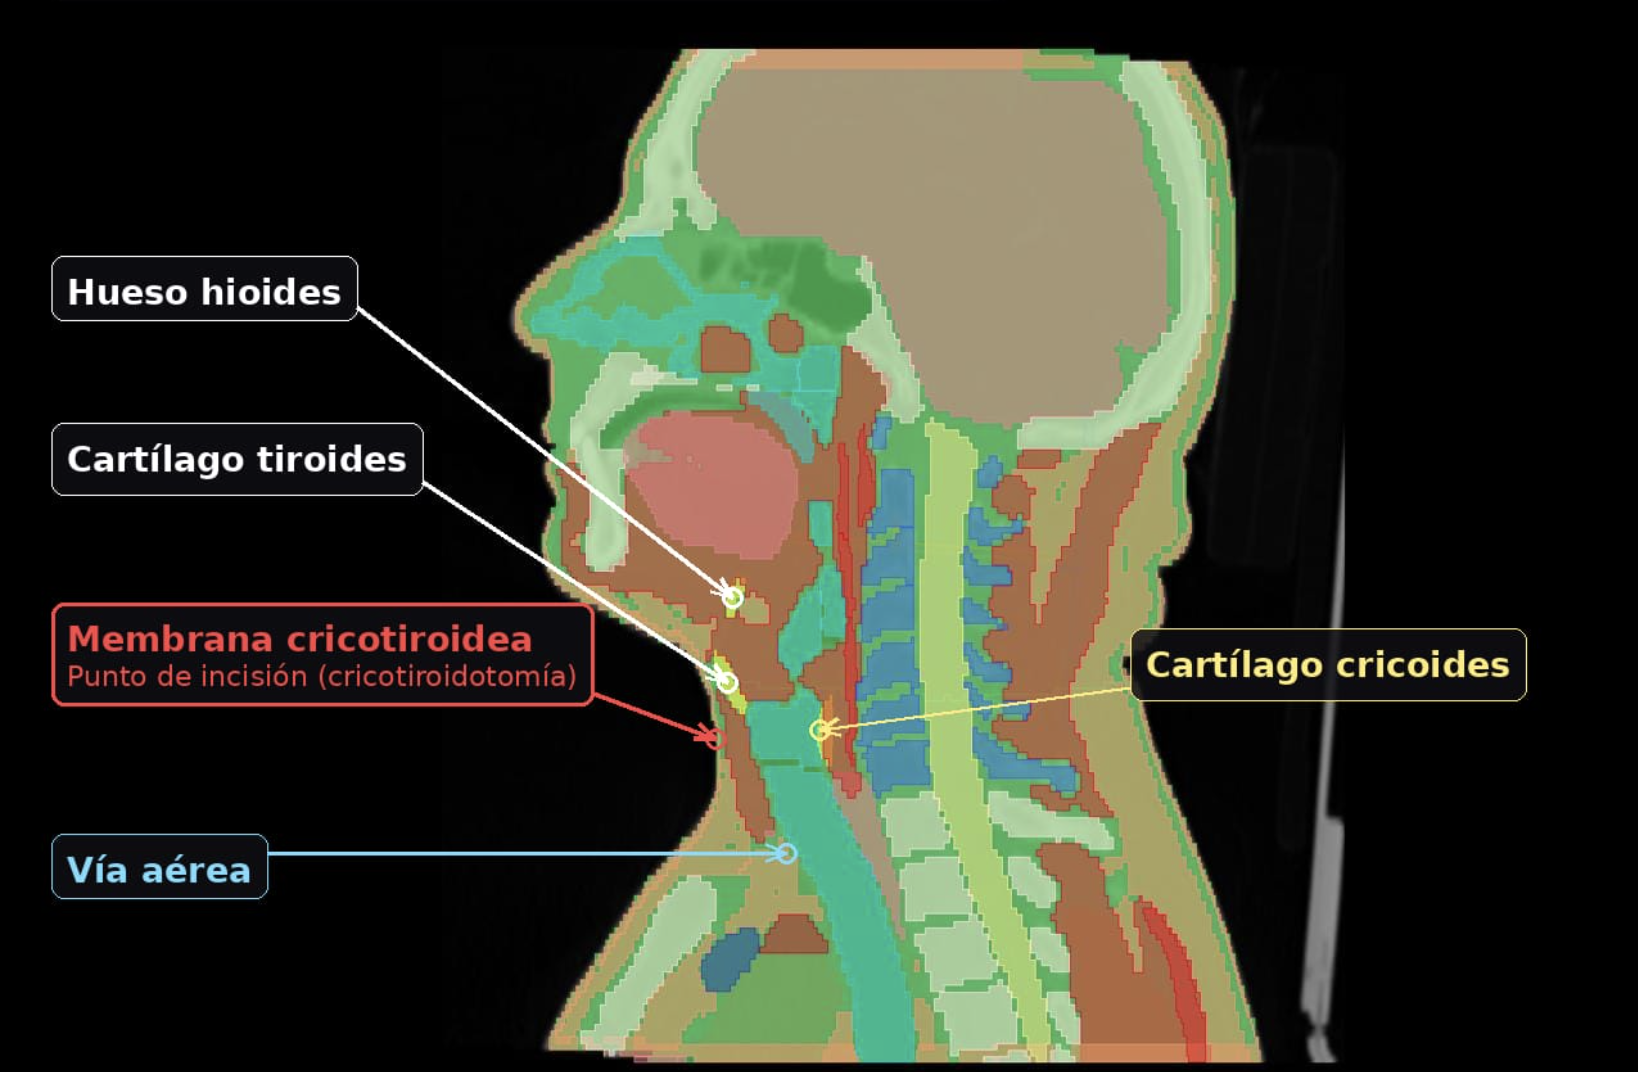
\includegraphics[width=0.8\textwidth]{imagenes/diagrama-sagital.png}
  \caption{Corte sagital de un cuello segmentado por el sistema, con las estructuras que delimitan el punto de incisión de la cricotiroidotomía: el hueso hioides, el cartílago tiroides, el cartílago cricoides y la vía aérea. La membrana cricotiroidea, señalada en rojo, es el punto donde se practica la incisión.}
  \vspace{2pt}
  \label{fig:diagrama-sagital}
  \begin{minipage}{\textwidth}
    \centering
    \normalsize Fuente: Elaboración propia.\\
  \end{minipage}
\end{figure}

Los fantomas comerciales disponibles reproducen una anatomía genérica y estandarizada, que no refleja la variabilidad anatómica real de los pacientes \citep{raekerjordan2022phantoms}. La región del cuello presenta diferencias considerables entre individuos según la edad, el índice de masa corporal, condiciones patológicas preexistentes o variantes congénitas. Un estudiante que practica la cricotiroidotomía decenas de veces sobre el mismo fantoma comercial desarrolla un conocimiento estático de la anatomía cervical, que puede resultar insuficiente al enfrentarse a la diversidad morfológica de los pacientes reales. La curva de aprendizaje de este procedimiento recién comienza a caracterizarse, y entre las brechas de entrenamiento identificadas figuran la familiarización anatómica insuficiente y el uso de maniquíes poco realistas \citep{mcmurray2023cricothyroidotomy}.\\

La impresión 3D ofrece una alternativa a esa limitación, ya que permite generar un fantoma a partir de las imágenes médicas de un paciente concreto, reproduciendo su anatomía individual. El insumo son tomografías computarizadas (TC), habitualmente convertidas al formato NIfTI, un estándar de almacenamiento de imágenes médicas volumétricas que guarda el escáner como una malla tridimensional de valores de intensidad junto con la información espacial necesaria para interpretarla. Producir el fantoma a partir de ese archivo implica una cadena de pasos técnicos: adquisición del escáner, segmentación de las estructuras anatómicas relevantes, exportación a modelos tridimensionales, preparación para impresión y fabricación física. De estos pasos, la segmentación es el principal cuello de botella: identificar y delimitar manualmente estructuras como la tráquea, los músculos escalenos, las glándulas parótidas o las vértebras cervicales en un escáner volumétrico exige varias horas de trabajo de un radiólogo o anatomista con experiencia. A modo de referencia, contornear un único caso de cabeza y cuello para planificación radioterápica toma en promedio cerca de 2,7 horas \citep{harari2010contouring}, y el conjunto de 64 estructuras de este proyecto es considerablemente más extenso que el habitual en ese contexto.\\

Esta dependencia del trabajo manual experto hace que la producción de fantomas personalizados sea hoy inviable a escala para las instituciones educativas. Cada nuevo caso clínico que se quisiera convertir en fantoma requeriría una inversión importante de tiempo de personal altamente calificado, lo que restringe el acceso a esta herramienta a casos excepcionales o a proyectos de investigación con financiamiento dedicado. La consecuencia práctica es que los estudiantes de medicina siguen entrenando, en su mayoría, sobre los mismos modelos genéricos, y pierden la oportunidad de exponerse a la variabilidad anatómica que encontrarán en su práctica clínica.\\

El presente proyecto nace de la identificación de esta brecha. Si se lograra automatizar la segmentación anatómica a partir de imágenes TC e integrar ese proceso en un flujo de trabajo que culmine en la impresión de un fantoma físico personalizado, sería posible producir modelos anatómicos diversos con un costo operacional sustancialmente menor. Ello permitiría a las instituciones médicas acceder a una biblioteca creciente de fantomas basados en casos reales, enriqueciendo la calidad del entrenamiento en procedimientos de urgencia como la cricotiroidotomía.\\

La Figura~\ref{fig:comparacion-flujo} contrasta el flujo manual con el propuesto.\\

\begin{figure}[H]
  \centering
  \includegraphics[width=0.9\textwidth]{diagramas/comparacion-flujo.pdf}
  \caption{Flujo manual de fabricación de fantomas, según la literatura, frente al flujo automatizado propuesto. La segmentación manual concentra el mayor costo de tiempo del proceso tradicional.}
  \label{fig:comparacion-flujo}
  \begin{minipage}{\textwidth}
    \centering
    \normalsize Fuente: Elaboración propia.\\
  \end{minipage}
\end{figure}

\section{ESTADO ACTUAL DEL PROBLEMA}

La fabricación de fantomas médicos personalizados mediante impresión 3D es un área de investigación activa, pero su adopción clínica masiva enfrenta barreras técnicas y operacionales que aún no se han resuelto de manera integral. El flujo de trabajo descrito en la literatura para convertir una imagen médica en un modelo físico comprende tres etapas: segmentación de la imagen, refinamiento de la malla e impresión 3D \citep{bucking2017workflow}. En la práctica, la segmentación se realiza habitualmente de forma manual o semiautomática en software especializado, como ITK-SNAP o 3D Slicer, una etapa laboriosa que demanda conocimiento anatómico avanzado \citep{tack2016review}. 3D Slicer es una plataforma de código abierto para el análisis, el procesamiento y la visualización tridimensional de imágenes médicas, ampliamente usada en investigación y extensible mediante módulos, sobre la que se construye el sistema de este trabajo. Si bien numerosos estudios demuestran la viabilidad técnica del concepto, con fantomas que reproducen con alta fidelidad estructuras como el árbol bronquial, el corazón o la columna vertebral, no proponen soluciones escalables que eliminen la dependencia del trabajo experto.\\

En cuanto a la segmentación automática, el avance más relevante de los últimos años ha sido TotalSegmentator, un modelo basado en la arquitectura nnU-Net \citep{isensee2021nnunet} entrenado sobre 1.204 tomografías computarizadas con anotaciones de 104 estructuras anatómicas \citep{wasserthal2023totalsegmentator}. La herramienta segmenta en pocos minutos un amplio conjunto de estructuras, principalmente de tronco, abdomen, huesos y vasos. Su desempeño se reporta mediante el coeficiente de Dice, una métrica que mide cuánto se superponen dos regiones, la predicha por el modelo y la delimitada por un especialista, y que vale 1 cuando ambas coinciden por completo y 0 cuando no comparten ningún punto. Sobre su conjunto de prueba, TotalSegmentator alcanza un Dice global de 0,943 \citep{wasserthal2023totalsegmentator}. Su tarea base, sin embargo, no fue concebida para la región cervical: las estructuras finas del cuello relevantes para la cricotiroidotomía no forman parte de esas 104 clases. Versiones posteriores de la herramienta incorporaron tareas especializadas de cabeza y cuello que cubren buena parte de esas estructuras; aun así, emplearla para generar un fantoma cervical completo exige orquestar varias de esas tareas y consolidar sus salidas, y un subconjunto de estructuras permanece sin cobertura. Caracterizar esa cobertura y resolver esa orquestación es parte del problema que aborda este trabajo.\\

Paralelamente han surgido modelos de segmentación basados en indicaciones visuales, como MedSAM, que adapta la arquitectura Segment Anything Model (SAM) de Meta al dominio médico mediante entrenamiento sobre un gran conjunto de imágenes médicas \citep{ma2024medsam}. MedSAM entrega buenos resultados en dos dimensiones cuando se le proveen recuadros delimitadores (\textit{bounding boxes}) que acotan la región de interés. Esa misma dependencia de indicaciones manuales lo aleja de un flujo completamente automático: sin intervención humana para definir las regiones, su desempeño se degrada de forma significativa.\\

A esta familia se suma YOLO, en su versión YOLOv8 con segmentación de instancias \citep{jocher2023yolov8}, un modelo de detección y segmentación en tiempo real de propósito general, no específico del dominio médico. Opera corte a corte sobre la imagen y prioriza la velocidad, lo que lo vuelve útil como referencia de contraste, aunque no fue concebido para delimitar estructuras anatómicas internas en volúmenes de TC.\\

En el ámbito de la fabricación, la disponibilidad de impresoras de costo relativamente accesible ha facilitado la producción de modelos anatómicos que diferencian los tejidos mediante filamentos de distinto color. El estado del arte va más allá y recurre a la impresión multimaterial, que distingue los tejidos no solo por color sino también por consistencia, acercándose a la sensación táctil del tejido real; esta capacidad, sin embargo, encarece el proceso, ya que las técnicas que reproducen distinta dureza por tejido son bastante más costosas que la impresión monomaterial \citep{chen2020multicolor}. En los Estados Unidos, la producción de modelos anatómicos personalizados a partir de imágenes de pacientes es ya una práctica establecida en el ámbito clínico, con costos por modelo que van desde menos de USD 100 hasta más de USD 1.000 según su finalidad \citep{sun2023lowcost}. Para el entrenamiento en cricotiroidotomía, diversos trabajos han mostrado que los modelos de vía aérea impresos en 3D constituyen una alternativa viable, reutilizable y de bajo costo frente a las dos opciones habituales, los maniquíes comerciales genéricos y las tráqueas porcinas, esta última limitada por su disponibilidad, su variabilidad entre animales y la necesidad de conservación biológica \citep{doucet2017trachea}. La fidelidad táctil de los materiales de impresión respecto del tejido blando real sigue siendo, en todo caso, una limitación reconocida. La integración de esta etapa de fabricación en un flujo automatizado que parta directamente de la imagen médica es el aspecto que la literatura revisada deja sin resolver.\\

En el contexto nacional, el acceso a fantomas personalizados para entrenamiento quirúrgico es limitado y tiende a concentrarse en centros académicos con mayores recursos. Los programas de simulación clínica suelen depender de materiales importados de alto costo o de modelos genéricos que no representan la diversidad anatómica de la población. Hasta donde se ha podido constatar, no existe una solución integrada, de código abierto y accesible, que permita a un equipo clínico sin formación en ingeniería generar un fantoma personalizado a partir de los datos clínicos de un paciente. Este trabajo se propone cubrir esa brecha.\\

\section{ALCANCE DEL PROYECTO}

El presente trabajo de titulación tiene como objetivo el diseño e implementación de un sistema que automatice la generación de fantomas anatómicos personalizados a partir de TC en formato NIfTI, orientado al entrenamiento en procedimientos de vía aérea de urgencia, con énfasis en la cricotiroidotomía. El sistema integra segmentación automática basada en inteligencia artificial, procesamiento y exportación de modelos tridimensionales e impresión 3D, conformando un flujo de trabajo completo y operable por equipos clínicos sin formación en procesamiento de imágenes.\\

El proyecto abarca el diseño y la evaluación de un módulo de segmentación automática que opera sobre escáneres TC. Para fundamentar su construcción se evaluaron tres herramientas de segmentación (TotalSegmentator, MedSAM y YOLO) sobre diez casos reales de escáneres cervicales, contrastando su salida con una segmentación de referencia de 64 estructuras anatómicas preparada por un radiólogo especialista. La evaluación consideró la cobertura anatómica alcanzada por cada herramienta, su concordancia con la referencia (medida mediante el coeficiente de Dice y la intersección sobre la unión, IoU) y el tiempo de procesamiento por caso. A ello se sumó un criterio de carácter eliminatorio: la capacidad de segmentar sin indicaciones manuales por estructura, sin la cual un flujo automatizado no es posible. La combinación de estos criterios permitió seleccionar de forma fundamentada la herramienta a integrar.\\

El flujo de trabajo completo se implementa en 3D Slicer mediante dos módulos personalizados de interfaz guiada, que abstraen la complejidad técnica para el usuario médico. El módulo de segmentación cubre la carga y el preprocesamiento del escáner TC, que incluye el recorte de los valores de intensidad atípicos. Estos valores se expresan en unidades Hounsfield (HU, por sus siglas en inglés) \citep{hounsfield1973}, la escala en que una TC codifica la densidad de cada punto del volumen, calibrada de modo que el agua vale 0 y el aire cercano a -1000. Enseguida, el módulo segmenta automáticamente las estructuras relevantes para el cuello y la cricotiroidotomía y consolida los segmentos resultantes. El módulo de corte y preparación para impresión permite seccionar el modelo con planos interactivos, centrarlo, orientar su base y escalarlo, generando los archivos STL definitivos. El formato STL describe la superficie de un objeto tridimensional como una malla de triángulos y es el que aceptan los programas de impresión 3D. Estos modelos se procesan finalmente en un laminador, el programa que traduce la malla en las instrucciones de recorrido y temperatura que ejecuta la impresora.\\

El alcance no incluye la certificación del fantoma como dispositivo clínico, la producción en serie ni la integración con sistemas hospitalarios o plataformas de gestión de imágenes médicas (PACS). Tampoco se contempla, en esta etapa, extender el flujo a regiones anatómicas distintas del cuello y la cabeza, si bien la arquitectura modular del sistema está diseñada para facilitar esa extensión futura. Los fantomas producidos en este trabajo se imprimen con un único material, diferenciando los tejidos por color pero no por consistencia. La impresión con materiales de distinta dureza por tipo de tejido queda planteada en la estructura de datos del sistema, pero su definición e implementación se dejan como trabajo futuro.\\
\chapter{Solución Planteada}
\label{ch:solucion-planteada}

\section{DESCRIPCIÓN DE LA SOLUCIÓN}

Frente a la falta de fantomas anatómicamente diversos para el entrenamiento de procedimientos de emergencia como la cricotiroidotomía, se propone un sistema que automatiza la generación de fantomas de cuello personalizados a partir de una TC de un paciente real. La solución reemplaza el flujo manual de segmentación, corrección y exportación, lento y dependiente de un operador con experiencia en herramientas de modelamiento 3D, por un flujo reproducible que un estudiante o docente de medicina puede ejecutar sin conocimientos de procesamiento de imágenes.\\

El sistema se organiza en cuatro etapas: a) ingreso de la TC en formato NIfTI; b) segmentación automática de las estructuras anatómicas relevantes para la vía aérea y el cuello (vértebras cervicales, cartílagos, tráquea, músculos, glándulas y tejidos blandos, entre otras); c) exportación de cada estructura segmentada a un archivo STL independiente; y d) preparación de los archivos STL en el laminador, donde se asigna a cada pieza el filamento con que se imprimirá. Las tres primeras se exponen al usuario final a través de dos módulos personalizados de 3D Slicer, que ocultan la complejidad interna del flujo (ejecución remota en GPU, consolidación de segmentos, mapeo de colores) detrás de una interfaz simple; la cuarta ocurre en el laminador, fuera del sistema. La Figura~\ref{fig:etapas-solucion} resume esta organización.\\

\begin{figure}[H]
  \centering
  \includegraphics[width=0.95\textwidth]{diagramas/etapas-solucion.pdf}
  \caption{Etapas de la solución, agrupadas por módulo. La preparación en el laminador queda fuera del sistema.}
  \label{fig:etapas-solucion}
  \begin{minipage}{\textwidth}
    \centering
    \vspace{5pt}
    \normalsize Fuente: Elaboración propia.\\
  \end{minipage}
\end{figure}

Para la etapa de segmentación automática se evaluaron tres alternativas (TotalSegmentator, MedSAM y YOLO) sobre una base de diez casos de cuello, contrastando su salida contra una segmentación de referencia elaborada por el radiólogo del proyecto, Héctor Henríquez. De esa evaluación se seleccionó TotalSegmentator \citep{wasserthal2023totalsegmentator} como motor de segmentación de la solución. El detalle de la comparación, y una limitación relevante en la naturaleza de la referencia empleada, se exponen en el Capítulo~\ref{ch:resultados}.\\

El sistema aplica dos criterios distintos para decidir qué estructuras conserva, según el propósito. En la comparación de modelos, descrita en el Capítulo~\ref{ch:resultados}, solo se retienen las estructuras que figuran en la segmentación de referencia, porque evaluar cada modelo exige contrastarlo contra un mismo conjunto común. En el flujo que genera el fantoma, en cambio, se conserva toda estructura que la segmentación produzca con contenido real, esté o no en esa referencia. Este segundo criterio es el que vuelve al sistema independiente de la imagen de entrada: no necesita una segmentación previa con la cual compararse, de modo que puede procesar casos nuevos por sí solo.\\

El cómputo de la segmentación, intensivo en uso de GPU, se ejecuta de forma remota en una máquina dedicada, comunicándose mediante SSH sobre una red privada. Esta decisión de arquitectura permite que los módulos de Slicer corran en un equipo sin GPU dedicada, ampliando el alcance de la herramienta a los computadores típicamente disponibles en un contexto docente.\\

\section{VIABILIDAD DE LA SOLUCIÓN}

La viabilidad de la solución se aborda desde lo técnico, lo económico y lo operacional.\\

En lo técnico, cada etapa del flujo se apoya en componentes que ya existen y están validados de forma independiente: TotalSegmentator para la segmentación, 3D Slicer como plataforma de visualización y desarrollo de módulos, y las herramientas estándar de impresión 3D para la fabricación. El aporte del trabajo no está en construir un modelo de segmentación desde cero, sino en orquestar estas piezas en un recorrido continuo y automatizado, que es justamente el eslabón que la literatura revisada deja sin resolver. Como cada componente es factible por separado, el riesgo técnico del conjunto es acotado.\\

En lo económico, el sistema se construye íntegramente sobre software de código abierto y sin costo de licencia, y opera sobre imágenes médicas que las instituciones de salud ya poseen, generadas en el curso normal de la atención clínica. Ello elimina el insumo más caro del flujo manual, que son las horas de trabajo de un radiólogo. Subsisten dos costos: el material de impresión, que es el único recurrente, y un equipo con GPU dedicada para la segmentación, que constituye una inversión inicial. Este último se comparte entre todos los casos que se procesen, por lo que su costo por fantoma decrece a medida que la herramienta se utiliza, y puede evitarse por completo ejecutando la segmentación en CPU a costa de un mayor tiempo de procesamiento.\\

En lo operacional, el usuario final no requiere formación en procesamiento de imágenes ni hardware especializado: interactúa con una interfaz guiada y el cómputo exigente se delega a una máquina remota. Esto mantiene el requerimiento de infraestructura del lado del usuario dentro de lo que un equipo docente ya tiene disponible.\\

\section{REQUISITOS}

\subsection{Requisitos funcionales}

\begin{enumerate}
  \item Permitir el ingreso de una tomografía computarizada de cuello en formato NIfTI desde el módulo de 3D Slicer. Se adopta NIfTI en lugar de DICOM porque el primero no conserva los metadatos identificatorios del paciente que el segundo incorpora, de modo que los casos procesados quedan anonimizados desde el ingreso.
  \item Ejecutar la segmentación automática de las estructuras anatómicas relevantes para la vía aérea y el cuello, delegando el cómputo a una máquina remota con GPU mediante conexión SSH.
  \item Consolidar los segmentos obtenidos descartando únicamente aquellos sin contenido (máscaras vacías), con independencia de la imagen de entrada.
  \item Permitir la visualización de las superficies tridimensionales generadas dentro de 3D Slicer.
  \item Permitir el corte y la reorientación de las estructuras mediante planos interactivos.
  \item Exportar cada estructura segmentada a un archivo STL independiente, listo para su impresión. El color con que se distingue cada tejido no forma parte del archivo STL, sino que se asigna manualmente en el laminador al preparar la impresión.
\end{enumerate}

\subsection{Requisitos operacionales}

\begin{enumerate}
  \item El sistema debe operar como un módulo instalable dentro de 3D Slicer (versión 5.10 o superior). El usuario final no requiere conocimientos de programación, si bien la puesta en marcha inicial supone seguir instrucciones técnicas de configuración, en particular el establecimiento de la conexión con el servidor remoto.
  \item El equipo del usuario no requiere GPU dedicada: el cómputo intensivo de la segmentación se ejecuta de forma remota, mediante una red privada y autenticación por llave SSH.
  \item La máquina remota debe contar con TotalSegmentator instalado y, para las tareas que lo requieran, con la licencia académica correspondiente activada.
  \item Los archivos STL resultantes deben poder cargarse en un laminador estándar sin requerir reparación previa de la malla.
  \item El tiempo total de una ejecución completa del módulo de segmentación, medido desde la carga de la TC hasta la exportación de los archivos STL e incluyendo las transferencias con la máquina remota, no debe superar los 30 minutos por caso.
  \item El costo de material por fantoma debe mantenerse muy por debajo del de los modelos anatómicos personalizados de referencia comercial.
\end{enumerate}

\section{CRITERIOS Y RESTRICCIONES}

\subsection{Criterios de calidad del producto}

\begin{enumerate}
  \item \textbf{Autonomía:} el motor de segmentación debe operar sin requerir indicaciones manuales por estructura (como recuadros delimitadores o marcas de referencia). Un modelo que dependa de ellas no puede sostener un flujo automatizado, ya que en un uso real esas indicaciones solo podrían provenir de una segmentación previa, que es justamente lo que el sistema busca evitar.
  \item \textbf{Cobertura de las estructuras del procedimiento:} el sistema debe producir las estructuras que delimitan el punto de incisión de la cricotiroidotomía, esto es, el cartílago tiroides, el cricoides, el hioides, la laringe y la tráquea. Sin ellas el fantoma pierde su propósito, por muchas otras estructuras que logre segmentar.
  \item \textbf{Usabilidad:} los módulos deben ocultar la complejidad técnica del flujo (ejecución remota, consolidación de segmentos, mapeo de colores) detrás de una interfaz simple, utilizable por personal médico sin formación en procesamiento de imágenes. El sistema entrega archivos STL, de modo que la etapa final de impresión supone un manejo básico de un laminador, competencia que queda fuera de lo que el sistema abstrae.
  \item \textbf{Portabilidad:} los módulos deben funcionar tanto en Windows como en macOS, sin depender de hardware gráfico especializado en el equipo local.
  \item \textbf{Mantenibilidad:} la separación entre el módulo de segmentación y el módulo de corte y exportación debe permitir modificar uno sin afectar el funcionamiento del otro.
  \item \textbf{Escalabilidad a otras regiones:} la arquitectura del flujo debe permitir procesar regiones anatómicas distintas del cuello reconfigurando las tareas de segmentación, sin modificar el diseño ni el código del sistema.
\end{enumerate}

\subsection{Criterios de selección del motor de segmentación}

La herramienta de segmentación se eligió mediante una comparación entre las tres alternativas consideradas. El criterio de autonomía enunciado más arriba opera como filtro previo: una herramienta que no lo satisface queda descartada, con independencia de su desempeño en cualquier otra dimensión. Sobre las que lo satisfacen, la comparación se estructuró en torno a los siguientes criterios, cuya definición formal se entrega en el Capítulo~\ref{ch:diseno-del-producto} y cuyos resultados se discuten en el Capítulo~\ref{ch:resultados}:

\begin{enumerate}
  \item \textbf{Cobertura anatómica:} cuántas de las estructuras de la referencia logra segmentar el modelo con contenido real.
  \item \textbf{Concordancia con la referencia clínica:} cuánto se superpone cada estructura predicha con su contraparte en la referencia, medida mediante el coeficiente de Dice y la intersección sobre la unión (IoU).
  \item \textbf{Tiempo de procesamiento:} el costo temporal por caso, considerando transferencia de archivos y segmentación.
\end{enumerate}

La denominación del segundo criterio como concordancia, y no como precisión, responde a una limitación en la naturaleza de la segmentación de referencia que se detalla en el Capítulo~\ref{ch:resultados} y que condiciona el alcance de lo que estas métricas permiten afirmar.\\

\subsection{Restricciones}

\begin{enumerate}
  \item La segmentación de referencia disponible para la evaluación fue elaborada por el radiólogo del proyecto con apoyo de segmentación automática, y no como una anotación manual independiente. Ello limita su uso como patrón de comparación imparcial entre modelos, circunstancia que se declara y se analiza en el Capítulo~\ref{ch:resultados}. No existió, dentro del alcance de este trabajo, acceso a una anotación independiente con la cual contrastar.
  \item Los diez casos de evaluación y la segmentación de referencia se mantienen únicamente en los computadores del equipo de trabajo; la infraestructura remota se utiliza exclusivamente para la segmentación del flujo del fantoma.
  \item El uso de la tarea \texttt{tissue\_types} de TotalSegmentator, que aporta las estructuras de tejido blando, está condicionado a una licencia académica gratuita, activada previamente en la máquina remota. Las demás tareas empleadas no requieren licencia.
  \item Los fantomas de este trabajo se imprimen con un único material, diferenciando los tejidos por color pero no por consistencia. La impresión con materiales de distinta dureza por tipo de tejido queda fuera del alcance y se plantea como mejora futura en el Capítulo~\ref{ch:resultados}.
  \item El sistema opera sobre escáneres de cuello y cabeza. Procesar otras regiones anatómicas requiere reconfigurar las tareas de segmentación, aunque la arquitectura del flujo no cambia.
\end{enumerate}

\subsection{Síntesis de requisitos}

La Tabla~\ref{tab:requisitos} reúne los requisitos y criterios anteriores junto a la forma en que se verifican. Su cumplimiento se evalúa uno a uno en el Capítulo~\ref{ch:resultados}.\\

\begin{table}[H]
  \centering
  \caption{Requisitos del sistema y su criterio de verificación.}
  \vspace{5pt}
  \label{tab:requisitos}
  \small
  \begin{tabular}{p{1.1cm} p{6.2cm} p{5.6cm}}
    \hline
    \textbf{ID} & \textbf{Requisito} & \textbf{Criterio de verificación} \\
    \hline
    RF1 & Ingreso de la TC en formato NIfTI, anonimizado & Carga archivos \texttt{.nii}/\texttt{.nii.gz} sin metadatos del paciente \\
    RF2 & Segmentación automática remota sobre GPU & Segmenta sin indicaciones manuales por estructura \\
    RF3 & Consolidación independiente de la imagen & Conserva las máscaras con contenido y descarta las vacías \\
    RF4 & Visualización 3D en Slicer & Muestra las superficies antes de exportar \\
    RF5 & Corte y reorientación con planos & Recorta el modelo antes de imprimir \\
    RF6 & Exportación de cada estructura a un archivo STL independiente & Genera un archivo STL por cada estructura conservada \\
    RO1 & Operación sin GPU local & El cómputo pesado corre en la máquina remota \\
    RO2 & STL imprimibles sin reparación & Se cargan en el laminador sin corregir la malla \\
    RO3 & Tiempo por caso $\leq$ 30 min & Tiempo total de una ejecución completa \\
    RO4 & Costo de material reducido & Costo de filamento por fantoma muy inferior al comercial \\
    CC1 & Autonomía (eliminatorio) & El motor segmenta sin indicaciones manuales \\
    CC2 & Cobertura de las estructuras del procedimiento & Produce cartílago tiroides, cricoides, hioides, laringe y tráquea \\
    CC3 & Usabilidad & Interfaz operable por personal médico sin formación en imágenes \\
    CC4 & Portabilidad & Los módulos funcionan en los sistemas operativos de destino \\
    CC5 & Escalabilidad a otras regiones & Procesa otra región cambiando el conjunto de tareas, sin rediseñar el flujo \\
    \hline
  \end{tabular}
  \begin{minipage}{\textwidth}
    \centering
    \vspace{5pt}
    \normalsize Fuente: Elaboración propia.\\
  \end{minipage}
\end{table}
\chapter{Diseño del Producto}
\label{ch:diseno-del-producto}

\section{ÍTEMS PRINCIPALES}

El producto desarrollado se compone de cuatro ítems principales que, en conjunto, conforman el recorrido completo desde la imagen médica hasta el fantoma físico imprimible: a) un módulo de segmentación automática; b) una infraestructura de cómputo remoto sobre una GPU dedicada que sustenta dicha segmentación; c) un módulo de corte y exportación; y d) el fantoma anatómico impreso, entendido como el entregable final del sistema. Los dos primeros ítems operan encadenados para producir las estructuras anatómicas segmentadas a partir del escáner; el tercero las adapta a las restricciones geométricas de la impresión 3D; y el cuarto materializa el resultado en un modelo físico apto para el entrenamiento clínico. Cada ítem se describe a continuación, dejando la forma en que se relacionan entre sí para la sección de arquitectura.\\

\subsection{Instalación y acceso a los módulos}

Ambos módulos se distribuyen en un mismo repositorio y se incorporan a 3D Slicer como módulos con \textit{script}, sin pasar por el gestor de extensiones. La instalación se realiza una sola vez: se descarga el repositorio y, en \textit{Edit → Application Settings → Modules}, se agrega la carpeta raíz (la que contiene los archivos \texttt{FantomaModule.py} y \texttt{CorteModule.py}) a la lista de rutas de módulos adicionales. Tras reiniciar la aplicación, ambos módulos quedan disponibles en el menú desplegable de módulos, bajo la categoría \textit{Proyecto Título}. En la Figura~\ref{fig:instalacion-modulos} se muestra como debiese resultar la correcta instalación del módulo.\\

\begin{figure}[H]
  \centering
  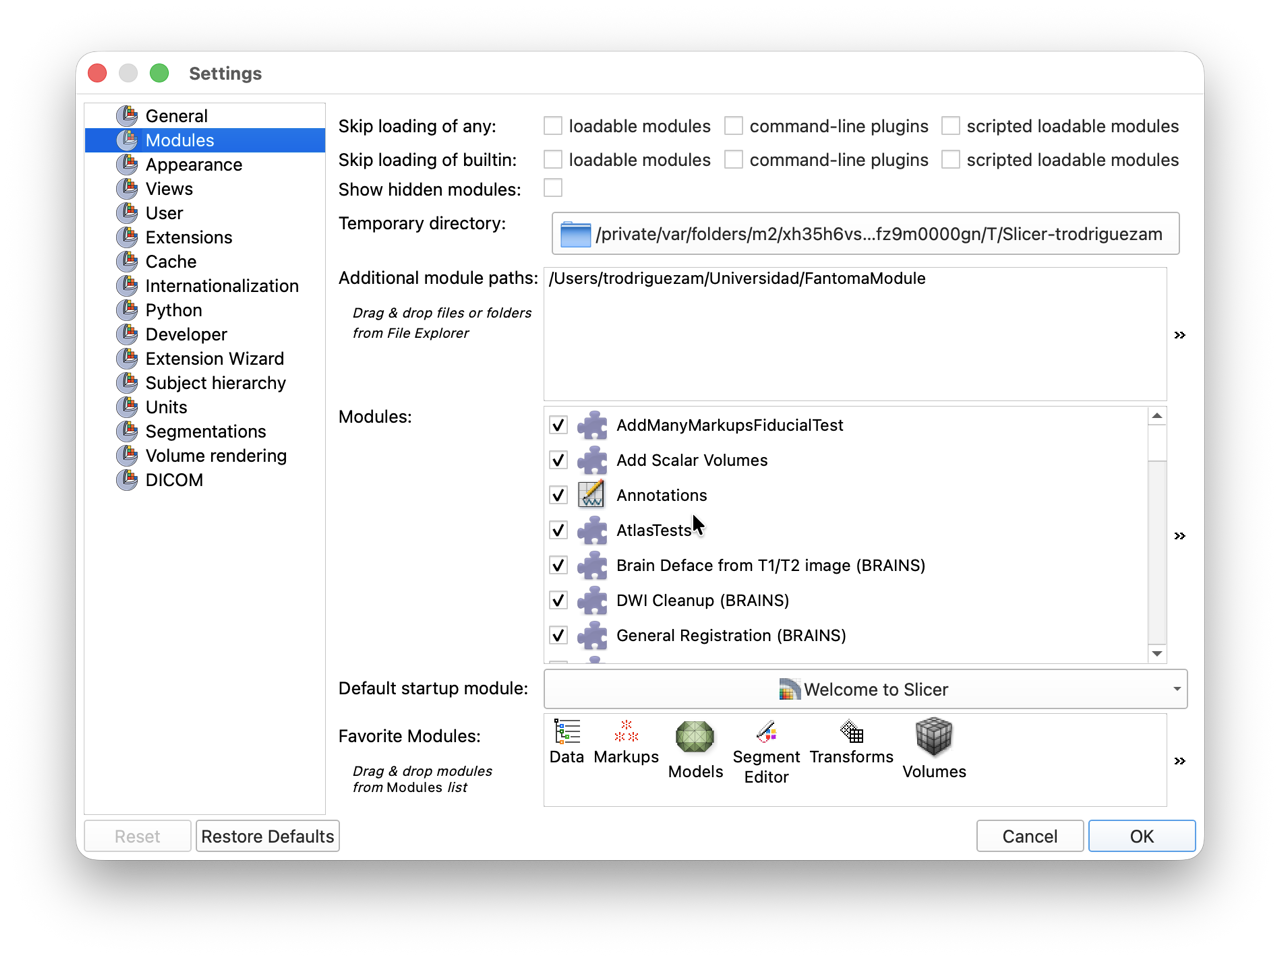
\includegraphics[width=0.8\textwidth]{imagenes/instalacion-modulos.png}
  \caption{Registro de los módulos en 3D Slicer mediante la ruta de módulos adicionales.}
  \label{fig:instalacion-modulos}
  \begin{minipage}{\textwidth}
    \centering
    \normalsize Fuente: Elaboración propia.\\
  \end{minipage}
\end{figure}

La interfaz general de 3D Slicer, la cual se puede apreciar en la Figura~\ref{fig:interfaz-general}, organiza la ventana en un panel que carga los módulos a la izquierda, donde cada módulo expone sus controles, y un área de visualización a la derecha con las vistas anatómicas y la vista tridimensional. Para operar el sistema, el usuario selecciona primero \textit{Segmentación Cuello} en el menú de módulos y, una vez generado el modelo, \textit{Corte 3D}, sin necesidad de recorrer el resto de los módulos que ofrece la aplicación.\\

\begin{figure}[H]
  \centering
  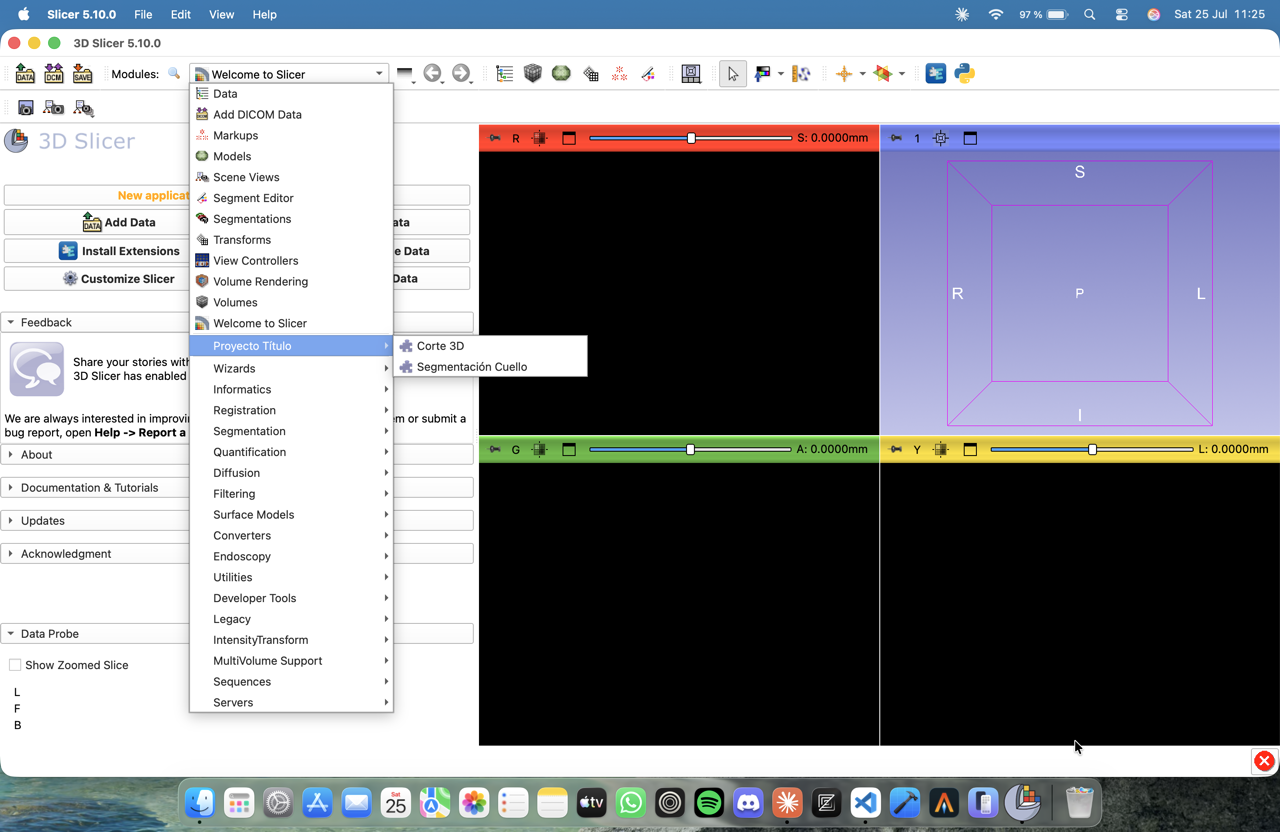
\includegraphics[width=0.8\textwidth]{imagenes/interfaz-general.png}
  \caption{Menú de módulos de 3D Slicer con la categoría \textit{Proyecto Título}, desde la que se accede a los dos módulos del sistema.}
  \label{fig:interfaz-general}
  \begin{minipage}{\textwidth}
    \centering
    \normalsize Fuente: Elaboración propia.\\
  \end{minipage}
\end{figure}

\subsection{Módulo de segmentación automática}

El módulo de segmentación, denominado \textit{Segmentación Cuello} dentro de 3D Slicer e identificado en el código como \texttt{FantomaModule}, constituye el punto de entrada del sistema. Su responsabilidad es transformar un escáner TC cervical, entregado en formato NIfTI (\texttt{.nii} o \texttt{.nii.gz}), en un conjunto de estructuras anatómicas segmentadas y coloreadas, visibles en la vista tridimensional de Slicer. El usuario selecciona el archivo de la TC, confirma el modo de procesamiento (remoto o local) e inicia la ejecución; el resto del flujo ocurre de forma automática.\\

Internamente, el módulo orquesta cuatro etapas sucesivas: el preprocesamiento de la imagen, la segmentación mediante TotalSegmentator \citep{wasserthal2023totalsegmentator}, la consolidación de las máscaras resultantes en un único conjunto de estructuras, y la carga de dichas estructuras en la escena con una asignación de color según el tipo de tejido. Toda esta complejidad permanece oculta tras una interfaz guiada, de modo que el operador no requiere conocimientos de procesamiento de imágenes ni de la herramienta de segmentación subyacente. Como salida, el módulo genera, por cada estructura detectada, tanto su máscara en formato NIfTI como su archivo STL, además de un reporte del proceso con las estructuras encontradas y los tiempos de ejecución. La exportación a STL está disponible, entonces, en los dos módulos: el de segmentación entrega un archivo por estructura apenas termina el proceso, y el de corte los vuelve a exportar tras recortar y reorientar el modelo.\\

\begin{figure}[H]
  \centering
  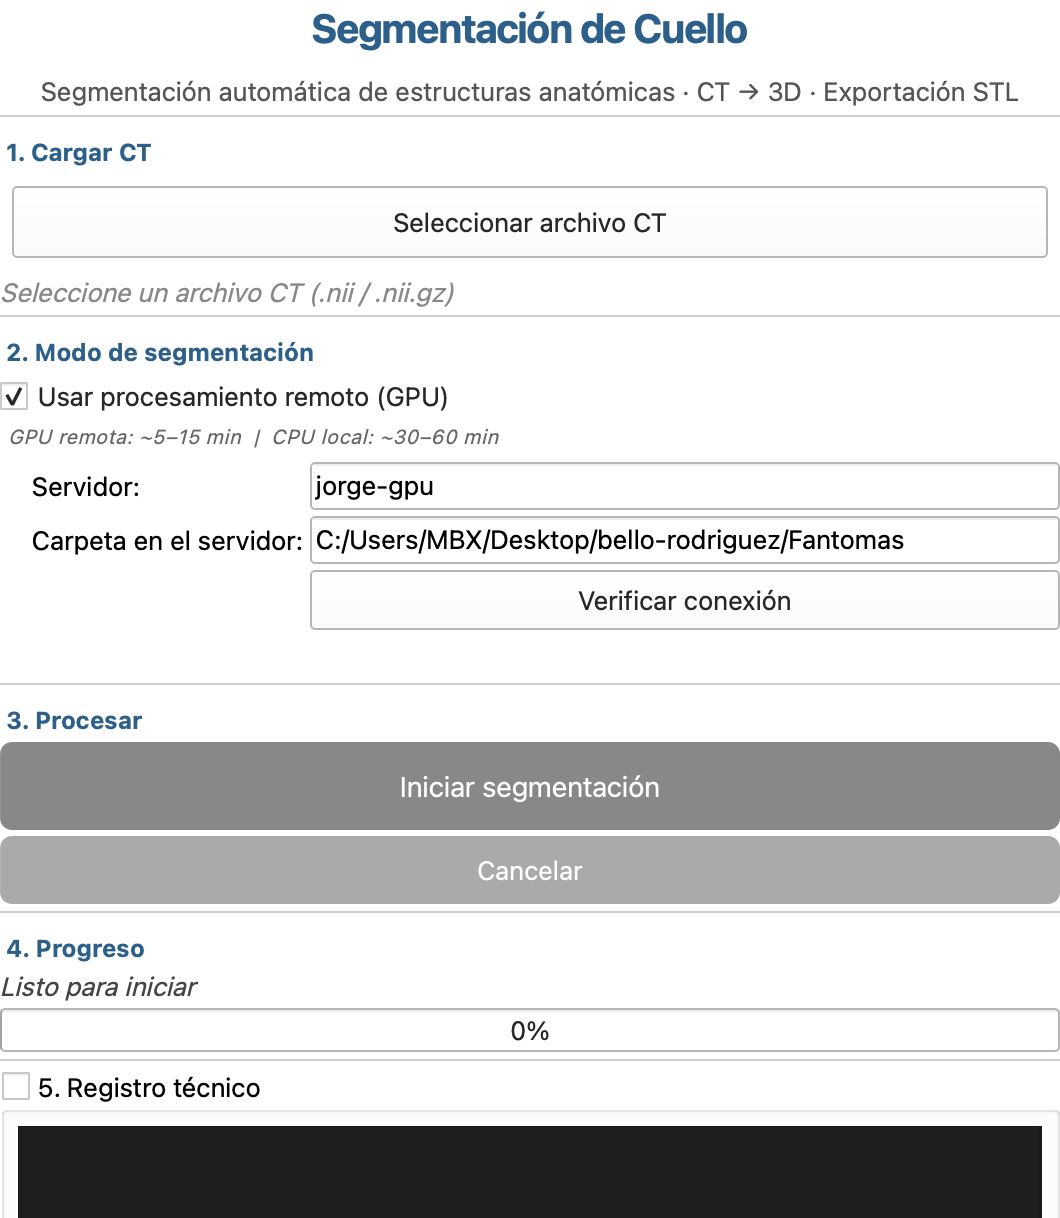
\includegraphics[width=0.6\textwidth]{imagenes/modulo-segmentacion.png}
  \caption{Interfaz del módulo de segmentación en 3D Slicer. El panel de control expone el selector del escáner TC, la elección del modo de procesamiento (remoto o local) y el botón de ejecución, junto al indicador de progreso del proceso.}
  \label{fig:modulo-segmentacion}
  \begin{minipage}{\textwidth}
    \centering
    \normalsize Fuente: Elaboración propia.\\
  \end{minipage}
\end{figure}

\subsection{Infraestructura de segmentación remota sobre GPU}

La segmentación con TotalSegmentator es computacionalmente exigente y se beneficia del uso de una unidad de procesamiento gráfico (GPU). Para evitar que el equipo clínico deba contar con hardware especializado, este ítem traslada el cómputo a una máquina dedicada con GPU, a la que el módulo de segmentación accede de forma transparente. La comunicación se realiza mediante SSH (\textit{Secure Shell}) y SCP (\textit{Secure Copy Protocol}) sobre una red privada virtual (VPN, \textit{Virtual Private Network}), lo que permite enviar el escáner preprocesado, ejecutar la segmentación en el servidor y recuperar las estructuras resultantes sin intervención manual del usuario.\\

Este ítem desacopla la carga de cómputo del puesto de trabajo del médico: el equipo local solo necesita ejecutar 3D Slicer y mantener la conexión con el servidor, mientras que el procesamiento pesado recae en la máquina remota. De este modo, el mismo flujo de trabajo puede ejecutarse desde equipos sin GPU dedicada, como los habituales en un contexto docente, lo que amplía la portabilidad del sistema.\\

\subsection{Módulo de corte y exportación}

El módulo de corte, denominado \textit{Corte 3D} en la interfaz y \texttt{CorteModule} en el código, toma la segmentación generada por el módulo anterior y la prepara para la impresión. Mediante planos de corte interactivos en las orientaciones axial, coronal y sagital, el usuario recorta los bordes del modelo hasta dejarlo con la forma y el tamaño adecuados para la cama de impresión; una opción de corte simétrico facilita conservar únicamente la zona central del cuello. Una vez aplicados los cortes, el módulo exporta el resultado a archivos STL, uno por cada estructura anatómica, listos para abrirse en un laminador y enviarse a la impresora.\\

\begin{figure}[H]
  \centering
  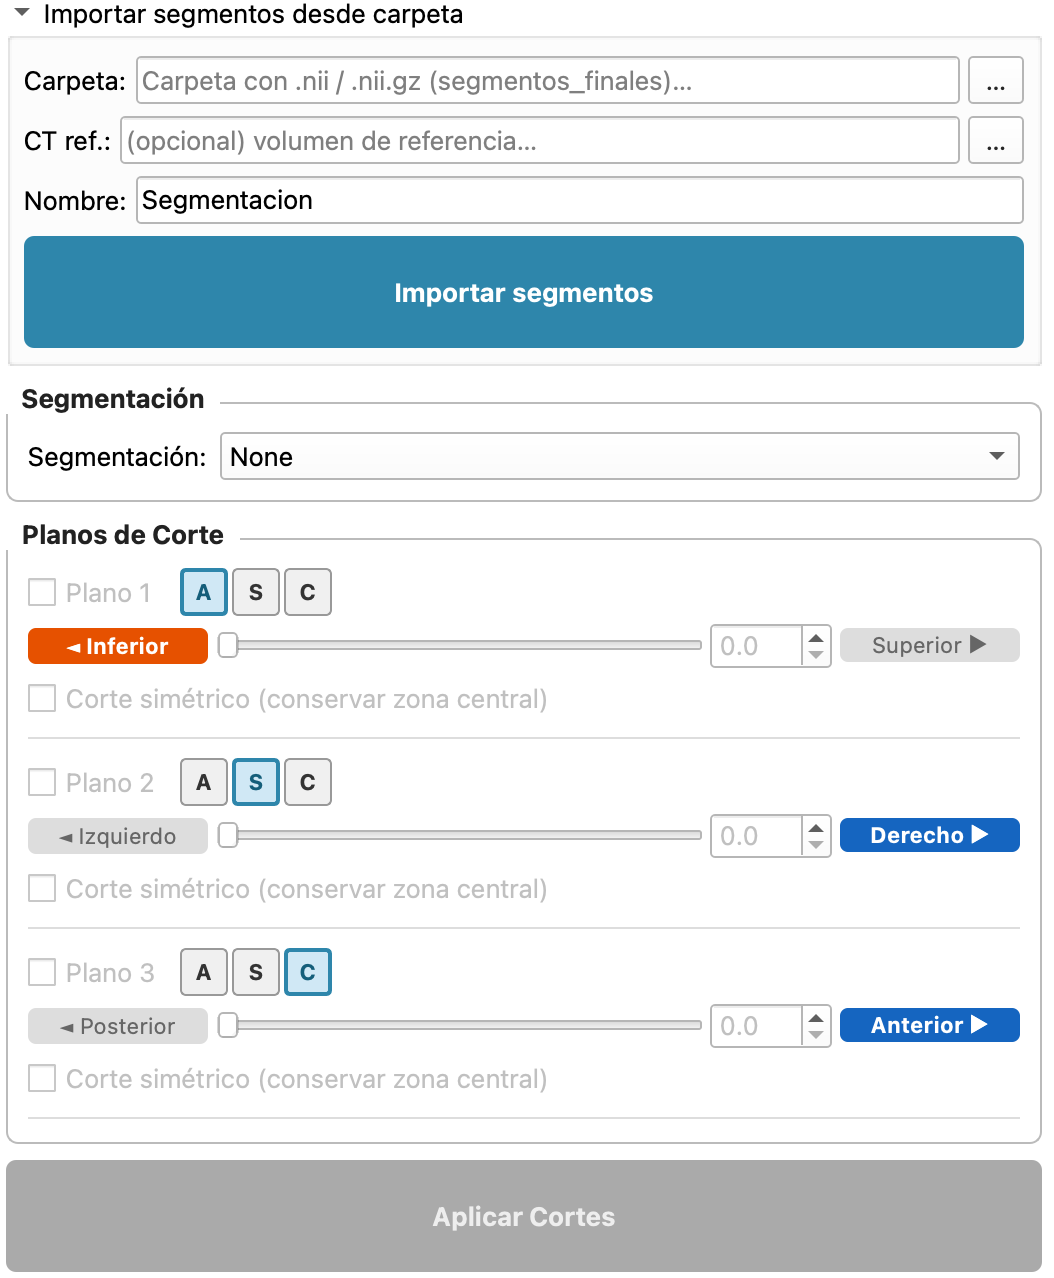
\includegraphics[width=0.49\textwidth]{imagenes/modulo-corte-1.png}
  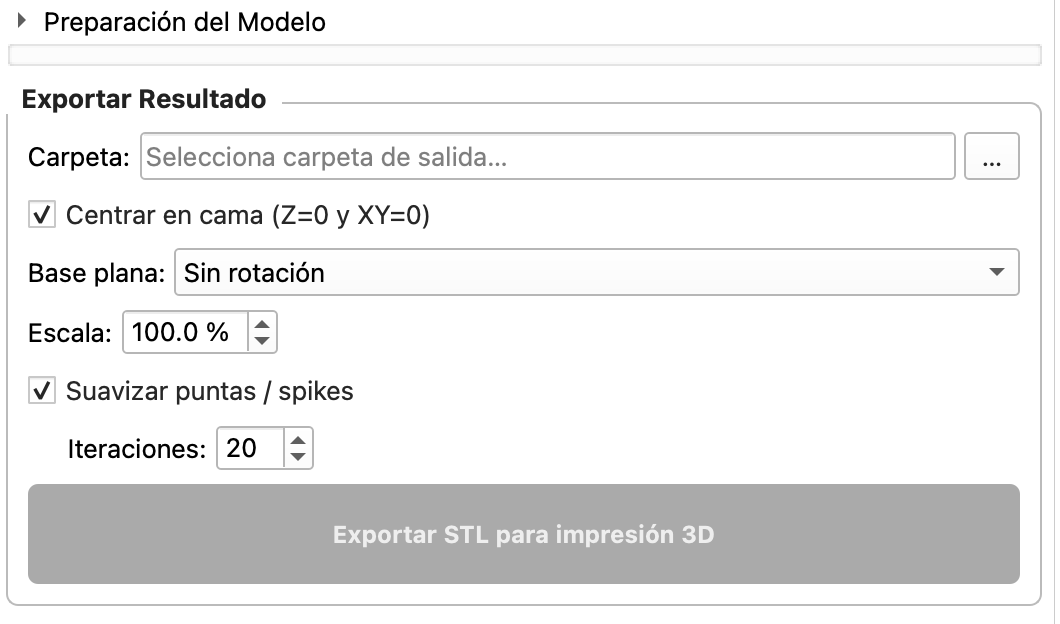
\includegraphics[width=0.49\textwidth]{imagenes/modulo-corte-2.png}
  \caption{Interfaz del módulo de corte en 3D Slicer, mostrada en dos partes por su extensión vertical: a la izquierda, los controles de los tres planos de corte y la opción de corte simétrico; a la derecha, la configuración de limpieza de malla (eliminación de fragmentos flotantes y cierre de superficie) previa a la exportación de los archivos STL.}
  \label{fig:modulo-corte}
  \begin{minipage}{\textwidth}
    \centering
    \normalsize Fuente: Elaboración propia.\\
  \end{minipage}
\end{figure}

\subsection{Fantoma anatómico impreso}

El último ítem corresponde al entregable físico del sistema: el fantoma de cuello impreso en 3D. A partir de los archivos STL exportados, la impresión produce un modelo en el que las distintas estructuras anatómicas se diferencian por color según el tipo de tejido. Las piezas obtenidas en este trabajo se imprimieron con un único material, de modo que la diferenciación es visual y no de consistencia; la asignación de materiales de distinta dureza por tejido queda planteada en la estructura de datos del sistema, pero su implementación se propone como trabajo futuro. Este fantoma constituye el objetivo final del producto, al proporcionar un modelo anatómicamente fiel y personalizado sobre el cual los estudiantes de medicina pueden reconocer la anatomía cervical de casos reales, sustituyendo los maniquíes genéricos por modelos que reflejan la diversidad morfológica de los pacientes.\\

\section{ARQUITECTURA DEL SISTEMA}

La arquitectura se organiza en torno a dos ejes de separación que ordenan el diseño y facilitan su mantenimiento. El primero distingue, dentro de cada módulo de 3D Slicer, la capa de presentación (la interfaz guiada con la que interactúa el usuario) de la capa de lógica, encapsulada en bibliotecas independientes (\texttt{FantomaModuleLib} y \texttt{CorteModuleLib}); de este modo, la interfaz puede modificarse sin alterar el procesamiento, y viceversa. El segundo eje distingue el cómputo local del remoto: la interacción del usuario y la preparación de los datos ocurren en el equipo clínico, mientras que la segmentación, intensiva en recursos, se ejecuta en un equipo con GPU. Esta doble separación permite que el sistema sea portable y que cada componente evolucione de forma aislada.\\

\subsection{Flujo de datos}

El recorrido de los datos sigue una secuencia lineal de etapas, desde el escáner TC de entrada hasta los archivos STL listos para imprimir. La Figura~\ref{fig:arquitectura} resume este flujo.\\

El proceso comienza cuando el usuario selecciona un escáner TC en formato NIfTI a través del módulo de segmentación. La imagen se preprocesa localmente, recortando los valores de intensidad atípicos que provienen del relleno del escáner, y el resultado se transfiere al servidor remoto mediante SCP. En el servidor, TotalSegmentator ejecuta sucesivamente las distintas tareas de segmentación sobre la GPU, generando una máscara por cada estructura anatómica reconocida. Estas máscaras se recuperan al equipo local, también por SCP, donde la etapa de consolidación las unifica en un único conjunto de estructuras. A continuación, las estructuras se cargan en la escena de 3D Slicer con una asignación de color según el tipo de tejido, momento en que el usuario puede inspeccionar visualmente el resultado en la vista tridimensional.\\

A partir de ese punto, el módulo de corte toma el control: el usuario recorta el modelo mediante planos interactivos, aplica las rutinas de preparación de malla y exporta cada estructura a su archivo STL correspondiente. Estos archivos abandonan el sistema y continúan su recorrido en el laminador, donde se generan las instrucciones de impresión.\\

\begin{figure}[H]
  \centering
  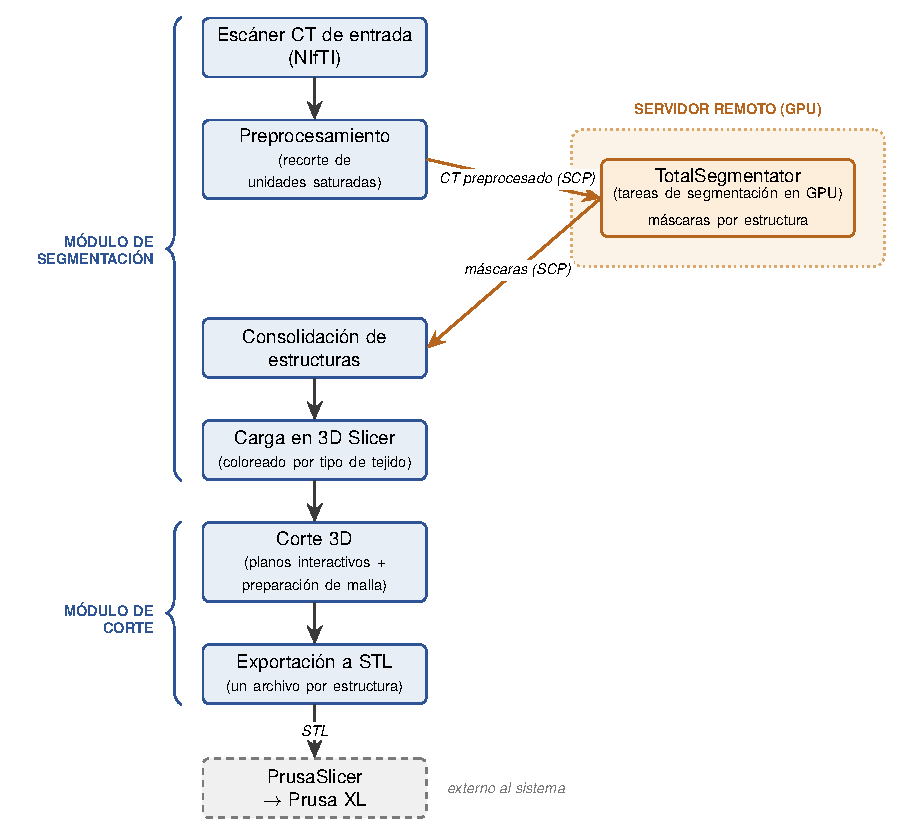
\includegraphics[width=0.9\textwidth]{diagramas/arquitectura.pdf}
  \caption{Flujo de datos del sistema, desde el escáner TC de entrada hasta los archivos STL. La segmentación se ejecuta en el servidor remoto con GPU; el resto del procesamiento ocurre en el equipo local.}
  \label{fig:arquitectura}
  \begin{minipage}{\textwidth}
    \centering
    \normalsize Fuente: Elaboración propia.\\
  \end{minipage}
\end{figure}

\subsection{Encadenamiento entre módulos}

Los dos módulos de Slicer no se comunican directamente entre sí, sino a través de la escena compartida de la aplicación. El módulo de segmentación deposita en la escena un nodo de segmentación con las estructuras detectadas; el módulo de corte, al activarse, ofrece al usuario seleccionar ese nodo como entrada. Esta comunicación indirecta mantiene a ambos módulos desacoplados: el módulo de corte puede operar sobre cualquier segmentación presente en la escena, no solo la generada por el flujo, y el módulo de segmentación no necesita conocer las operaciones posteriores de corte y exportación.\\

\subsection{Comunicación entre el equipo local y el servidor remoto}

La conexión entre el equipo clínico y el servidor con GPU se establece sobre una VPN, que asigna a ambos extremos una dirección estable dentro de una red cifrada, independiente de la red física en que se encuentren. Sobre esta red, el sistema utiliza SSH para ejecutar comandos en el servidor y SCP para transferir archivos en ambos sentidos, apoyándose en un alias de conexión configurado una sola vez en cada equipo. La autenticación se realiza mediante un par de claves, sin contraseñas interactivas, lo que permite que el módulo orqueste la segmentación remota de forma autónoma, sin intervención del usuario durante el proceso.\\

\section{IMPLEMENTACIÓN DE LA SOLUCIÓN}

La solución se implementó como dos módulos (\textit{scripted modules}) de 3D Slicer, escritos en Python. Toda la interfaz se construye de forma programática, sin archivos de descripción de interfaz externos, y la lógica de procesamiento se aísla en bibliotecas independientes (\texttt{FantomaModuleLib} y \texttt{CorteModuleLib}), para que la capa de presentación y la de procesamiento puedan evolucionar por separado. A continuación se detallan las decisiones de implementación de cada componente, así como las métricas con que se evaluó el motor de segmentación.\\

\subsection{Preprocesamiento y segmentación}

La primera etapa del módulo de segmentación es un preprocesamiento que recorta los valores de la imagen al rango $[-1024, 3071]$ unidades Hounsfield, con el fin de descartar valores atípicos provenientes del relleno del escáner que, de no corregirse, degradan la segmentación posterior.\\

El rango corresponde a la codificación de doce bits con signo en que los escáneres de TC almacenan nativamente la densidad. Ninguna estructura anatómica humana lo excede, ya que el hueso cortical más denso rara vez supera los 2.000 HU; los valores por sobre ese límite provienen de material metálico, como amalgamas dentales o implantes, o de artefactos del relleno del escáner. La operación satura esos valores en el extremo del rango en lugar de eliminarlos, de modo que no se pierde ningún vóxel, cada punto del volumen tridimensional y equivalente al píxel en tres dimensiones, ni, por tanto, ninguna estructura.\\

En la práctica, la mayoría de los escáneres ya vienen dentro de este rango, en cuyo caso el módulo detecta que el recorte no altera la imagen y reutiliza el archivo original, evitando reescribir y volver a transferir un volumen idéntico.\\

Una tarea de TotalSegmentator es un modelo especializado, entrenado para segmentar un grupo determinado de estructuras anatómicas. La segmentación se obtiene ejecutando sucesivamente siete de estas tareas, cuyas máscaras se complementan para cubrir el conjunto de estructuras de interés del cuello. Ninguna tarea aislada basta: la tarea base no fue entrenada para la región cervical, y las estructuras que definen el punto anatómico de la cricotiroidotomía (el cartílago tiroides y el cricoides) provienen de una tarea especializada de cabeza y cuello. La Tabla~\ref{tab:tasks} detalla el aporte de cada una.\\

\begin{table}[H]
  \centering
  \caption{Tareas de TotalSegmentator ejecutadas por el módulo de segmentación y estructuras que aporta cada una.}
  \label{tab:tasks}
  \begin{tabular}{p{3.4cm}p{7.2cm}c}
    \hline
    \textbf{Tarea} & \textbf{Estructuras principales que aporta} & \textbf{Licencia} \\
    \hline
    \texttt{total} & Vértebras cervicales y torácicas, tráquea, esófago, glándula tiroides, grandes vasos, médula espinal & No \\
    \texttt{body} & Contorno corporal, tronco, extremidades y piel & No \\
    \texttt{head\_glands\_ cavities} & Ojos, cristalinos, nervios ópticos, glándulas parótidas y submandibulares, faringe, cavidades nasales, paladar & No \\
    \texttt{head\_muscles} & Maseteros, temporales, pterigoideos, lengua, digástricos & No \\
    \texttt{headneck\_bones\_ vessels} & Cartílago tiroides, cricoides, hioides, laringe, carótidas internas, yugulares internas & No \\
    \texttt{headneck\_muscles} & Esternocleidomastoideos, constrictores faríngeos, trapecios, platisma, escalenos, esternotiroideos, tirohioideos, prevertebrales & No \\
    \texttt{tissue\_types} & Músculo esquelético, grasa subcutánea, grasa de torso & Sí \\
    \hline
  \end{tabular}
  \begin{minipage}{\textwidth}
    \centering
    \normalsize Fuente: Elaboración propia a partir de \citep{wasserthal2023totalsegmentator}.\\
  \end{minipage}
\end{table}

De las siete tareas, solo \texttt{tissue\_types} está sujeta a licencia. Se trata de una licencia académica gratuita, que se activa una única vez en la máquina remota y habilita el uso no comercial de sus resultados. Su incorporación no es accesoria: aporta las tres estructuras de tejido blando (músculo esquelético y los dos compartimentos grasos) que ninguna otra tarea cubre y que son necesarias para que el fantoma reproduzca el volumen real del cuello por sobre las estructuras profundas.\\

Una restricción técnica relevante es que TotalSegmentator no puede ejecutarse dentro del hilo principal de Slicer, debido a un conflicto entre su mecanismo interno de creación de procesos y el entorno de la aplicación. Para resolverlo, la segmentación se delega a un proceso independiente, lanzado mediante un \textit{script} auxiliar escrito en disco e invocado como subproceso; mientras este se ejecuta, un hilo de fondo mantiene la interfaz receptiva y reporta el progreso al usuario.\\

\subsection{Consolidación de las estructuras}

Una vez generadas todas las máscaras, la etapa de consolidación las unifica en un único conjunto de estructuras aplicando un filtro espacial. El filtro revisa el contenido de cada máscara y conserva toda aquella con al menos un vóxel no nulo, descartando las que quedaron completamente vacías porque la estructura no aparece en el volumen analizado. La decisión depende, entonces, de lo que la imagen realmente contiene y no de una lista fija de nombres de estructuras esperadas. Esa es la diferencia con el filtro que emplea la comparación de modelos, que exige que el nombre de cada estructura figure en la referencia: el filtro espacial deja pasar cualquier estructura con contenido, incluidas las que la referencia no anota, y es lo que hace al sistema independiente de la imagen de entrada. Las estructuras que no aparecen en el volumen analizado quedan vacías y se eliminan solas, sin necesidad de mantener un catálogo que actualizar cada vez que se agrega una tarea.\\

La decisión tiene una consecuencia deliberada: el módulo conserva todas las estructuras con contenido real, incluidas aquellas que no forman parte del conjunto de referencia. Ese conjunto sirve para comparar modelos, no para limitar la salida del sistema. El alcance de esta diferencia se cuantifica en el Capítulo~\ref{ch:resultados}.\\

Cada estructura conservada se carga en la escena con un color asignado según su tipo de tejido. La asignación se resuelve mediante un diccionario que asocia el nombre de cada estructura a un color, definido en la configuración del módulo y no en el código de procesamiento, así ampliarlo no exige tocar la lógica del flujo. Los colores agrupan las estructuras por familia anatómica: tonos óseos para vértebras, cráneo y costillas; rojizos para la musculatura; azules para el sistema venoso y rojos para el arterial; y un amarillo destacado para los cartílagos laríngeos, que marcan el punto de incisión. Esta asignación cumple dos funciones: facilita el reconocimiento anatómico en la vista tridimensional y determina el color con que cada pieza se imprimirá, ya que se conserva al exportar los archivos STL. El diccionario cubre tanto las estructuras del conjunto de referencia como las adicionales que el flujo conserva, entre ellas los cartílagos tiroides y cricoides, el hioides y la laringe, para que el punto de incisión de la cricotiroidotomía quede visualmente diferenciado en el fantoma. Cuando una estructura carece de entrada, recibe un color por defecto y el hecho se registra, lo que permite detectar las que aportan las tareas de segmentación sin que el flujo se interrumpa.\\

El módulo emite además un reporte en formato JSON con las estructuras detectadas, las descartadas por máscara vacía y los tiempos de cada etapa. Este registro no responde a un requisito del producto, ya que el usuario clínico no lo necesita para operar el sistema, sino a una necesidad de este trabajo: es el instrumento que permitió medir la cobertura y los tiempos que se reportan en el Capítulo~\ref{ch:resultados}.\\

\subsection{Ejecución remota sobre GPU}

La ejecución remota se implementó utilizando exclusivamente herramientas estándar (SSH y SCP), disponibles en los dos sistemas operativos de destino (macOS y Windows), sin dependencias adicionales. La secuencia consiste en crear un directorio de trabajo en el servidor, transferir la TC preprocesada, ejecutar el \textit{script} de segmentación sobre la GPU, recuperar las estructuras resultantes y eliminar los archivos temporales del servidor.\\

Durante la implementación se debieron resolver incompatibilidades propias de la comunicación entre sistemas operativos distintos, en particular en la codificación de caracteres de la salida de los comandos remotos, que se normalizó a UTF-8 para evitar fallos de lectura. Asimismo, se forzó el vaciado inmediato de los \textit{buffers} de salida de los subprocesos, para que el progreso reportado al usuario refleje el avance real y no aparente bloqueos.\\

\subsection{Módulo de corte y exportación}

El módulo de corte opera sobre el nodo de segmentación presente en la escena. Para cada estructura obtiene su representación de superficie mediante la interfaz correspondiente de Slicer y le aplica los planos de corte definidos por el usuario. Antes de exportar, se ejecutan rutinas de preparación de la malla: limpieza de triángulos degenerados, eliminación de fragmentos flotantes y cierre de superficies. Estas rutinas son las que permiten que el modelo resultante sea imprimible sin reparación previa, uno de los requisitos operacionales del sistema.\\

La exportación a STL contempla tres transformaciones geométricas configurables: el centrado del modelo sobre la base de impresión, dejando su cara inferior en la cota cero; la rotación según el plano de corte que se haya utilizado como base; y un factor de escala. El resultado es un archivo STL por estructura, con la orientación y posición adecuadas para abrirse directamente en un laminador.\\

\subsection{Evaluación del motor de segmentación}

La elección de TotalSegmentator surgió de una evaluación comparativa frente a otras dos alternativas (MedSAM y YOLO) sobre diez casos reales de escáneres cervicales. Como término de comparación se dispuso de una segmentación de referencia de 64 estructuras anatómicas, elaborada por un radiólogo especialista. A diferencia del flujo del fantoma, esta evaluación exige una correspondencia estricta entre cada estructura predicha y su contraparte en la referencia, ya que sin ella no es posible calcular métricas de superposición.\\

El primer criterio de selección, enunciado en el Capítulo~\ref{ch:solucion-planteada}, es de carácter eliminatorio y no requiere cálculo alguno: el modelo debe segmentar sin indicaciones manuales por estructura. MedSAM no lo satisface, ya que opera a partir de recuadros delimitadores que acotan cada región de interés; en la evaluación estos se extrajeron de la propia referencia, lo que constituye una condición favorable que en un uso real no existiría. YOLO sí opera sin indicaciones, pero requiere un emparejamiento posterior entre sus detecciones y las estructuras esperadas, que también se resolvió recurriendo a la referencia. Ambas alternativas se evaluaron de todos modos, con el fin de cuantificar cuánto se aproximan a una segmentación clínicamente validada aun operando en condiciones privilegiadas.\\

Los criterios cuantitativos se apoyan en dos métricas de superposición volumétrica. Sea $P$ el conjunto de vóxeles segmentados por el modelo y $G$ el conjunto de vóxeles de la segmentación de referencia. El coeficiente de Dice se define como:

\begin{equation}
\mathrm{Dice}(P,G) = \frac{2\,|P \cap G|}{|P| + |G|}
\end{equation}

y mide la superposición entre ambas regiones, ponderando al doble la intersección. La intersección sobre la unión se define como:

\begin{equation}
\mathrm{IoU}(P,G) = \frac{|P \cap G|}{|P \cup G|}
\end{equation}

y constituye una medida más estricta de la misma superposición. Ambos coeficientes toman valores en el intervalo $[0,1]$, donde $1$ indica coincidencia perfecta, y están relacionados de forma monótona mediante $\mathrm{IoU} = \mathrm{Dice}\,/\,(2 - \mathrm{Dice})$.\\

Una particularidad de estas métricas exige atención. Cuando $P$ y $G$ están ambos vacíos, el denominador se anula y el coeficiente queda indefinido. La convención habitual \citep{taha2015metrics}, adoptada también por la implementación empleada en este trabajo, es asignarle en ese caso el valor $1$, entendiendo que el modelo acertó al no predecir nada donde no había nada que predecir. Esta convención es razonable de forma aislada, pero introduce un sesgo cuando se promedia sobre un conjunto de estructuras que no siempre están presentes en el volumen analizado, cuestión que se aborda en el Capítulo~\ref{ch:resultados}.\\

A estas dos métricas se sumaron dos criterios de carácter práctico: la cobertura anatómica, entendida como la proporción de las estructuras de referencia que el modelo logra segmentar con contenido no vacío, y el tiempo de procesamiento por caso. Los resultados de esta evaluación, junto con una limitación relevante en la naturaleza de la segmentación de referencia, se presentan y discuten en el Capítulo~\ref{ch:resultados}.\\
\chapter{Resultados Obtenidos y Posibles Mejoras}
\label{ch:resultados}

% ---------------------------------------------------------------------------
% TIEMPOS DEL FLUJO COMPLETO
% PENDIENTE: recalcular tras corregir el desempaquetado local. Los valores
% actuales corresponden a una medición previa y NO reflejan el desglose real
% (el cuello de botella medido es la escritura local, no la descarga).
\newcommand{\tPreproc}{4 min}
\newcommand{\tEnvio}{50 s}
\newcommand{\tSeg}{5 min}
\newcommand{\tLocal}{15 min}
\newcommand{\tLimpieza}{3 min}
\newcommand{\tTotal}{28 min}
% ---------------------------------------------------------------------------

\section{RESULTADOS OBTENIDOS}

Los resultados se organizan en tres planos. El primero caracteriza la segmentación de referencia, hallazgo que condiciona cómo debe leerse todo lo demás. El segundo es la evaluación comparativa de las tres herramientas de segmentación y el fundamento de la elección del motor. El tercero es el comportamiento del sistema integrado: cobertura anatómica, tiempo de procesamiento y generación del fantoma imprimible.\\

\subsection{Naturaleza de la segmentación de referencia}

La evaluación se planteó originalmente contra una segmentación manual independiente. Al auditar los datos entregados, sin embargo, se constató que la referencia no fue elaborada desde cero: el radiólogo del proyecto ejecutó TotalSegmentator sobre los diez casos y revisó y corrigió manualmente su salida, práctica habitual en el ámbito clínico. Este hecho se declara aquí porque condiciona la interpretación de las métricas de superposición y, por tanto, la validez del argumento con que se selecciona el motor de segmentación.\\

La consecuencia es directa. Un coeficiente de Dice calculado entre TotalSegmentator y esta referencia no mide precisión frente a una anotación independiente, sino concordancia entre el modelo y una versión corregida de su propia salida. Lo mismo ocurre con la cobertura: al derivar de TotalSegmentator, la referencia contiene por construcción aquello que TotalSegmentator detecta. Ninguna de estas dos métricas puede arbitrar de forma imparcial entre TotalSegmentator y las alternativas, y así se las reporta en lo que sigue: como medidas de concordancia, no de precisión.\\

Esta constatación no invalida la evaluación, pero traslada su peso. Lo que la comparación sí permite establecer es si las alternativas consideradas son capaces de reproducir de forma autónoma una segmentación validada clínicamente. Los criterios que fundamentan la selección del motor, expuestos al cierre de esta comparación, no dependen de las métricas de superposición.\\

\subsection{Correcciones aplicadas por el especialista}

La circunstancia anterior habilita un análisis que no estaba previsto y que resulta más informativo que las métricas originales. Comparando la salida cruda de TotalSegmentator con la referencia corregida es posible identificar dónde intervino el especialista, lo que delimita empíricamente en qué estructuras la segmentación automática resulta confiable y en cuáles requiere supervisión clínica. La Tabla~\ref{tab:correcciones} resume el resultado.\\

\begin{table}[H]
  \centering
  \caption{Divergencia entre la salida automática y la referencia corregida por el especialista, promediada sobre nueve casos.}
  \label{tab:correcciones}
  \begin{tabular}{lc}
    \hline
    \textbf{Estructura} & \textbf{Divergencia} \\
    \hline
    Vértebra C1 & 26,4\% \\
    Vértebra C5 & 19,8\% \\
    Vértebra C6 & 19,4\% \\
    Vértebra C3 & 19,4\% \\
    Vértebra C4 & 19,2\% \\
    Vértebra C7 & 16,8\% \\
    Vértebra C2 & 16,3\% \\
    Tráquea     & 11,7\% \\
    \hline
    El resto de las estructuras & $\leq$ 0,7\% \\
    \hline
  \end{tabular}
  \begin{minipage}{\textwidth}
    \centering
    \normalsize Fuente: Elaboración propia.\\
  \end{minipage}
\end{table}

El patrón de correcciones es nítido. La musculatura, las glándulas, los ojos, la faringe, los tejidos grasos, la piel y el contorno corporal presentan divergencias iguales o inferiores al 0,7\%, y el especialista las aceptó sin retoques. Las correcciones se concentran en las siete vértebras cervicales y en la tráquea, con divergencias de entre el 11,7\% y el 26,4\%. La separación entre ambos grupos es tajante: ninguna estructura queda en un rango intermedio.\\

La lectura clínica es que la segmentación automática de tejido blando alcanza una calidad que un especialista considera aceptable sin retoques, mientras que las estructuras óseas cervicales y la vía aérea requieren revisión. Que estas últimas sean precisamente las que delimitan el punto de incisión de la cricotiroidotomía tiene una implicancia operativa concreta, recogida entre las mejoras propuestas.\\

Dos exclusiones deben señalarse. El cráneo se apartó de este análisis porque presenta una divergencia sistemática, con la salida automática entre un 19\% y un 30\% más extensa que la referencia en todos los casos. La regularidad del sesgo es incompatible con una corrección manual y apunta a una diferencia de configuración: la referencia contiene, además, seis estructuras craneofaciales que las tareas empleadas en este trabajo no producen, lo que indica que el especialista ejecutó un conjunto de tareas distinto. Asimismo, se excluyó uno de los diez casos, cuyo campo de visión reducido deja varias estructuras de referencia con contenido residual o nulo, lo que distorsiona cualquier promedio.\\

\subsection{Comparación cuantitativa de los modelos de segmentación}

Con las salvedades anteriores, la Tabla~\ref{tab:comparacion} resume el desempeño de los tres modelos sobre los diez casos.\\

\begin{table}[H]
  \centering
  \caption{Concordancia de los tres modelos con la segmentación de referencia, sobre el total de estructuras con contenido real.}
  \label{tab:comparacion}
  \begin{tabular}{lcccc}
    \hline
    \textbf{Modelo} & \textbf{Cobertura} & \textbf{Dice} & \textbf{IoU} & \textbf{Tiempo} \\
    \hline
    TotalSegmentator & 90,8\% & 0,892 & 0,879 & $\sim$4,9 min \\
    MedSAM           & 81,4\% & 0,553 & 0,415 & $\sim$5,3 min \\
    YOLOv8x-seg      & 13,4\% & 0,108 & 0,085 & $\sim$0,8 min \\
    \hline
  \end{tabular}
  \begin{minipage}{\textwidth}
    \centering
    \normalsize Fuente: Elaboración propia.\\
  \end{minipage}
\end{table}

Las cifras de TotalSegmentator deben leerse con la reserva ya expuesta: al derivar la referencia de su propia salida, su ventaja en estas columnas está sobredeterminada y no constituye evidencia de superioridad. Lo informativo de la tabla es lo contrario de lo esperable: ni MedSAM ni YOLO se aproximan a una segmentación clínicamente validada, ni siquiera operando en condiciones privilegiadas.\\

Ambos modelos se evaluaron en condiciones favorables. MedSAM no es un segmentador autónomo: opera a partir de recuadros delimitadores que acotan cada estructura, y en esta evaluación esos recuadros se extrajeron de la propia segmentación de referencia. Es decir, se le indicó dónde estaba cada estructura antes de pedirle que la segmentara. En un uso real esa información no existe, ya que solo podría provenir de una segmentación previa, que es justamente lo que el sistema busca producir. A YOLO se le aplicó un emparejamiento por solapamiento contra esa misma referencia. Aun así, MedSAM alcanza un Dice de 0,553 y YOLO uno de 0,108, con mediana nula.\\

La Figura~\ref{fig:dice-por-caso} muestra esa concordancia caso a caso. TotalSegmentator se mantiene alto y parejo en los diez, mientras que MedSAM oscila en la zona media y YOLO permanece bajo en todos.\\

La diferencia entre los tres modelos también se aprecia directamente en su salida sobre un mismo caso. La Figura~\ref{fig:comparacion-cualitativa} muestra el resultado de los tres sobre el caso 5, una vez procesados por el módulo de corte. TotalSegmentator reconstruye un volumen anatómicamente coherente, en el que las estructuras conservan su forma y posición. MedSAM produce un volumen fragmentado, sin correspondencia anatómica reconocible, pese a haber operado con los recuadros delimitadores extraídos de la referencia. YOLO genera un conjunto de láminas desconectadas entre sí, consecuencia directa de procesar el escáner corte a corte sin coherencia tridimensional. La comparación visual confirma lo que las métricas indican: solo TotalSegmentator entrega una segmentación utilizable para construir un modelo físico.\\
 
\begin{figure}[H]
  \centering
  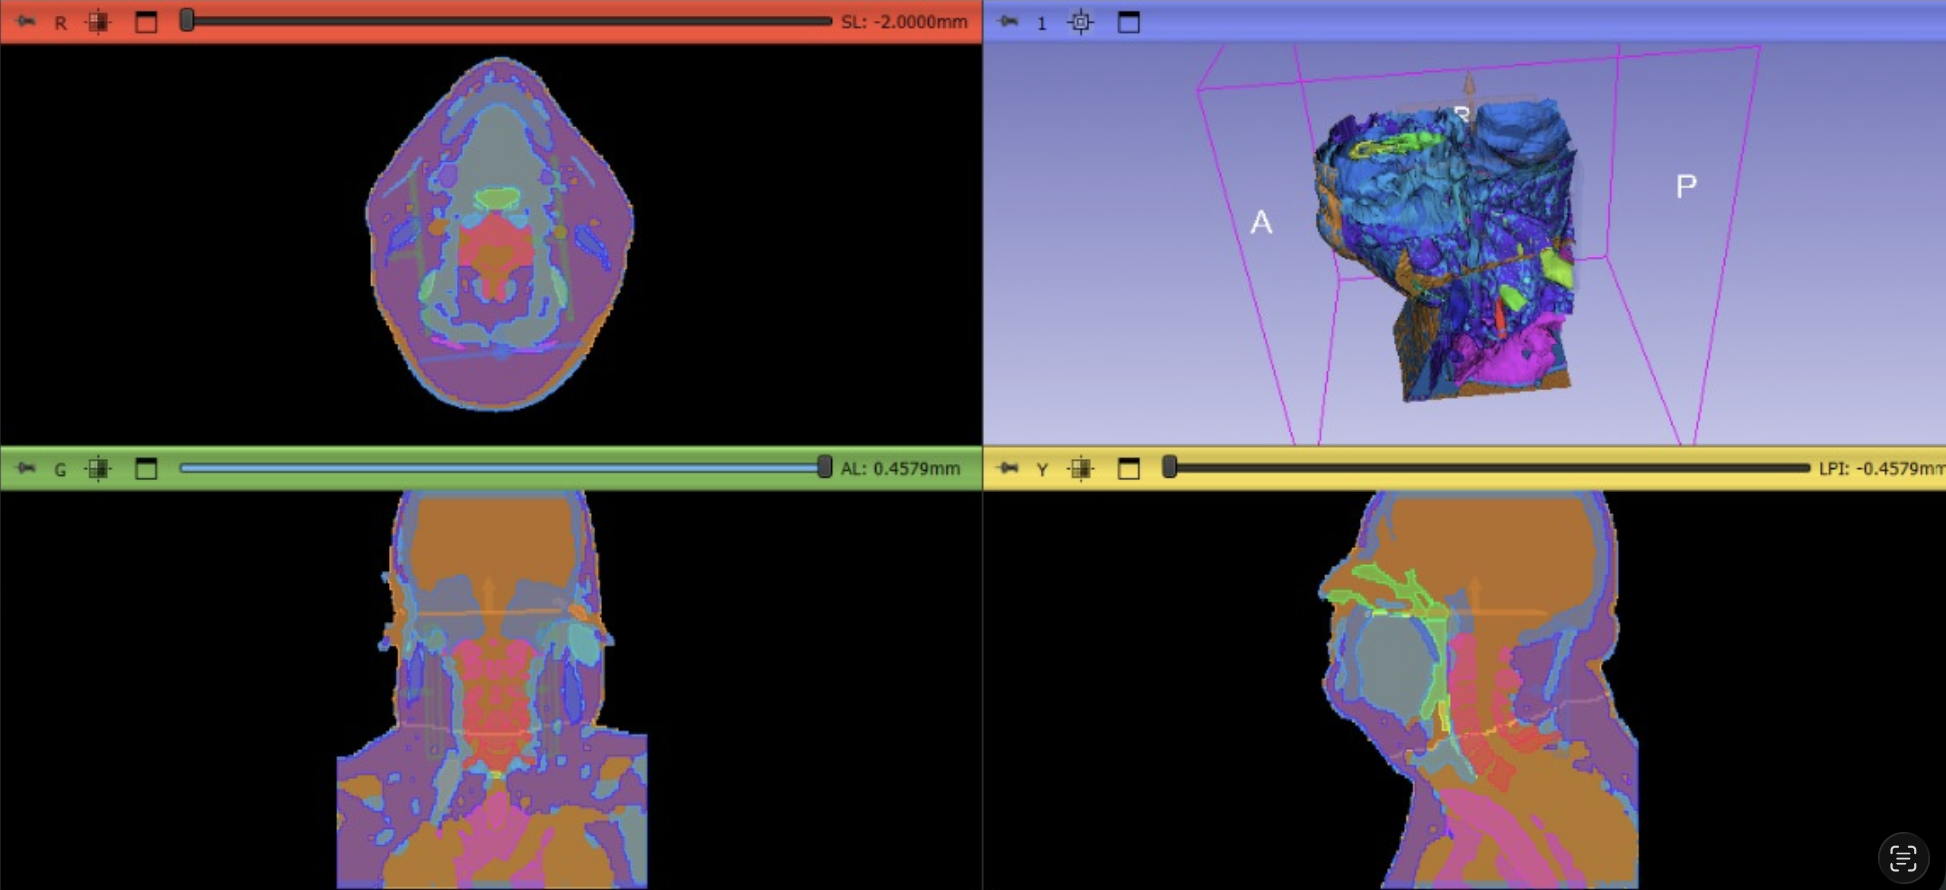
\includegraphics[width=0.49\textwidth]{imagenes/segmentacion-ts.png}\hfill
  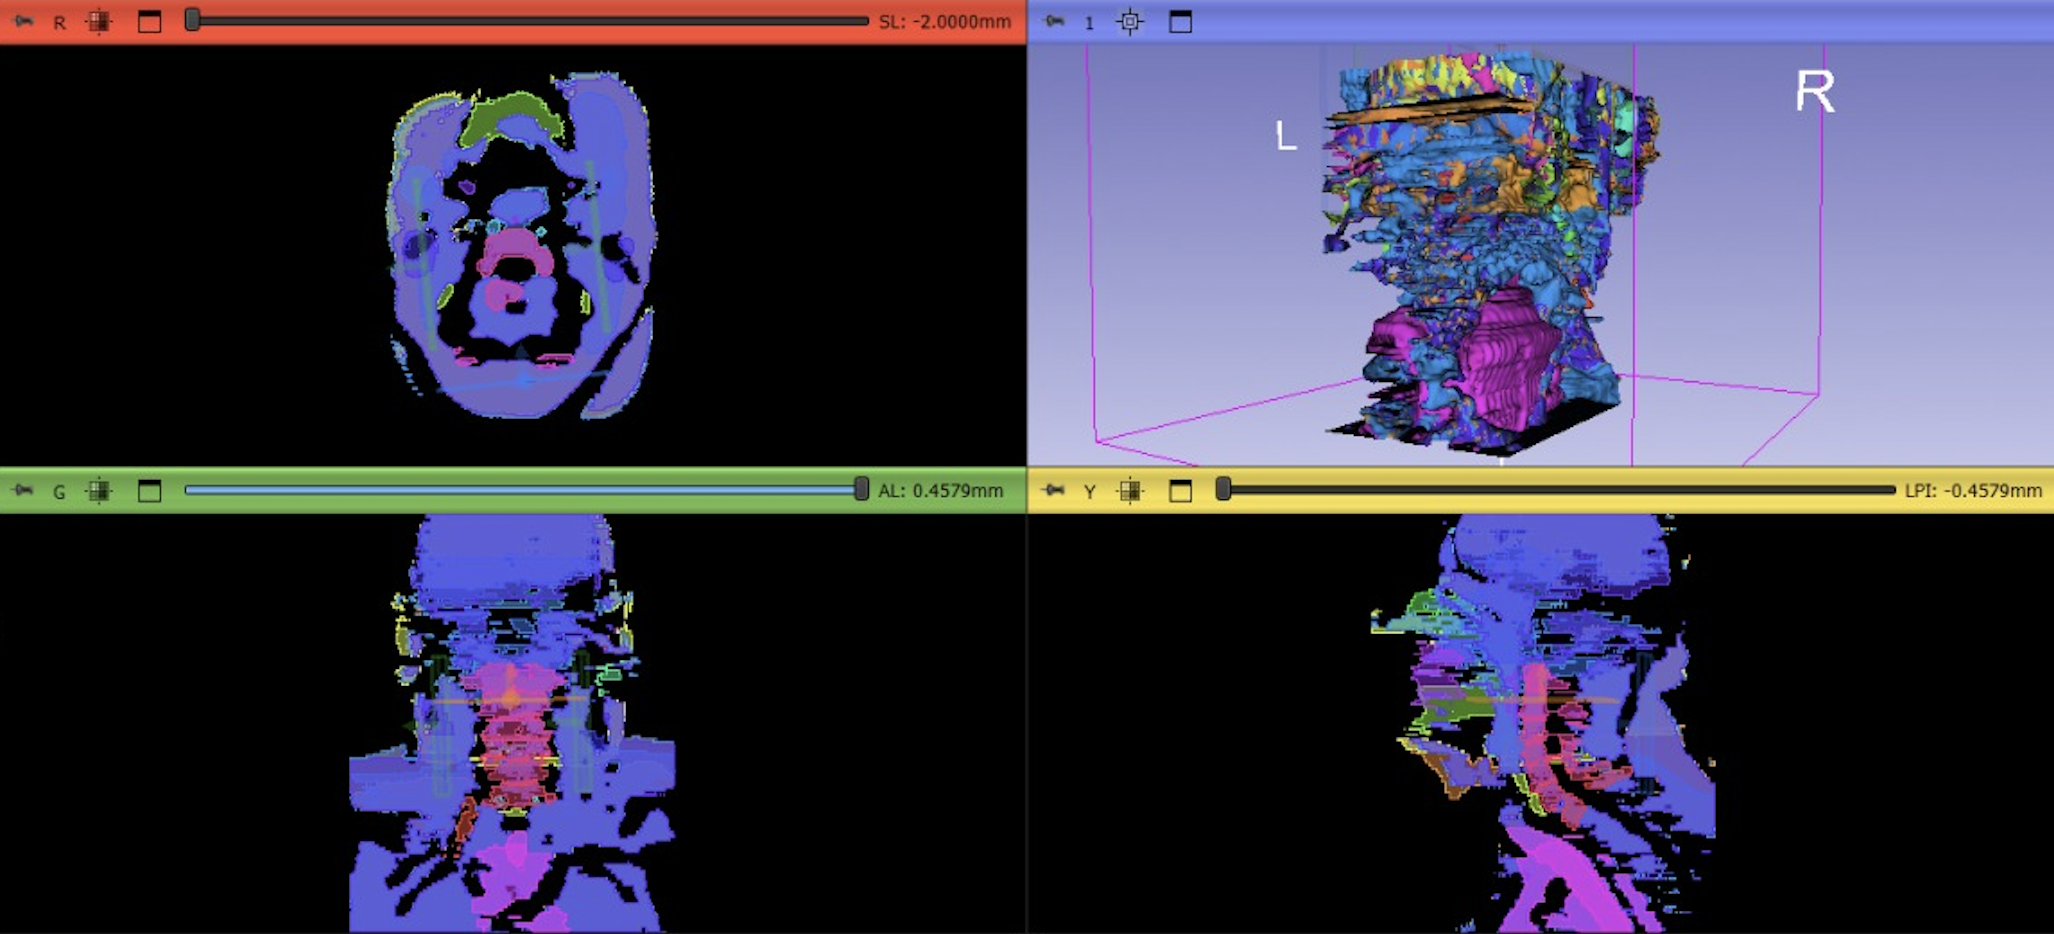
\includegraphics[width=0.49\textwidth]{imagenes/segmentacion-medsam.png}\hfill
  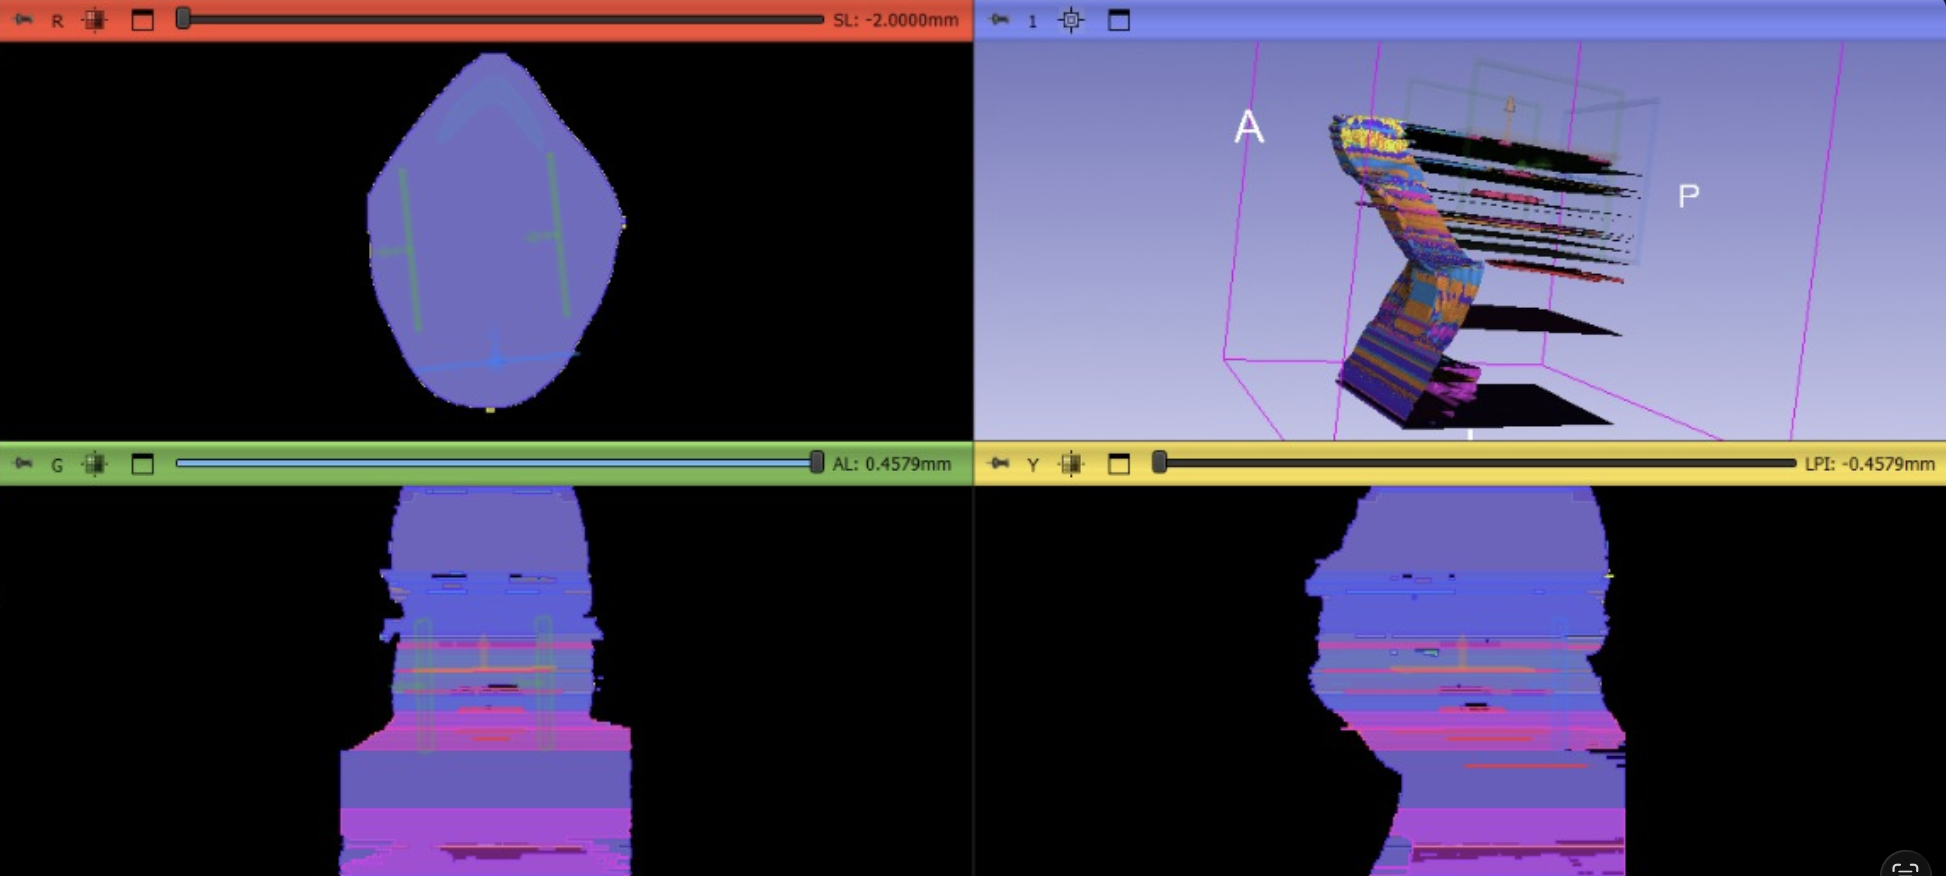
\includegraphics[width=0.49\textwidth]{imagenes/segmentacion-yolo.png}
  \caption{Salida de los tres modelos sobre el caso 5, procesada por el módulo de corte. De izquierda a derecha: TotalSegmentator, con estructuras anatómicas coherentes; MedSAM, con un volumen fragmentado pese a operar con recuadros de la referencia; y YOLO, que produce láminas desconectadas por procesar el escáner corte a corte.}
  \label{fig:comparacion-cualitativa}
  \begin{minipage}{\textwidth}
    \centering
    \normalsize Fuente: Elaboración propia.\\
  \end{minipage}
\end{figure}

Un artefacto de la métrica requirió corrección antes de calcular estas cifras. El coeficiente de Dice está indefinido cuando la máscara predicha y la de referencia están ambas vacías, y la convención habitual le asigna el valor 1, entendiendo que el modelo acertó al no predecir nada donde no había nada. En la práctica, no todos los escáneres cubren la misma región anatómica: en uno de los diez casos, solo 43 de las 64 estructuras de referencia tienen contenido real. Sin filtrar, un modelo que no segmenta nada obtiene una puntuación perfecta sobre cada estructura ausente. Por ello, todas las métricas de este capítulo se calculan únicamente sobre las estructuras con referencia no vacía en cada caso. El filtro, adoptado por rigor, perjudica en realidad a las alternativas: TotalSegmentator predice algo en algunas de esas estructuras ausentes, lo que cuenta como falso positivo, mientras que MedSAM y YOLO no predicen nada y se beneficiaban de la puntuación trivial.\\

\begin{figure}[H]
  \centering
  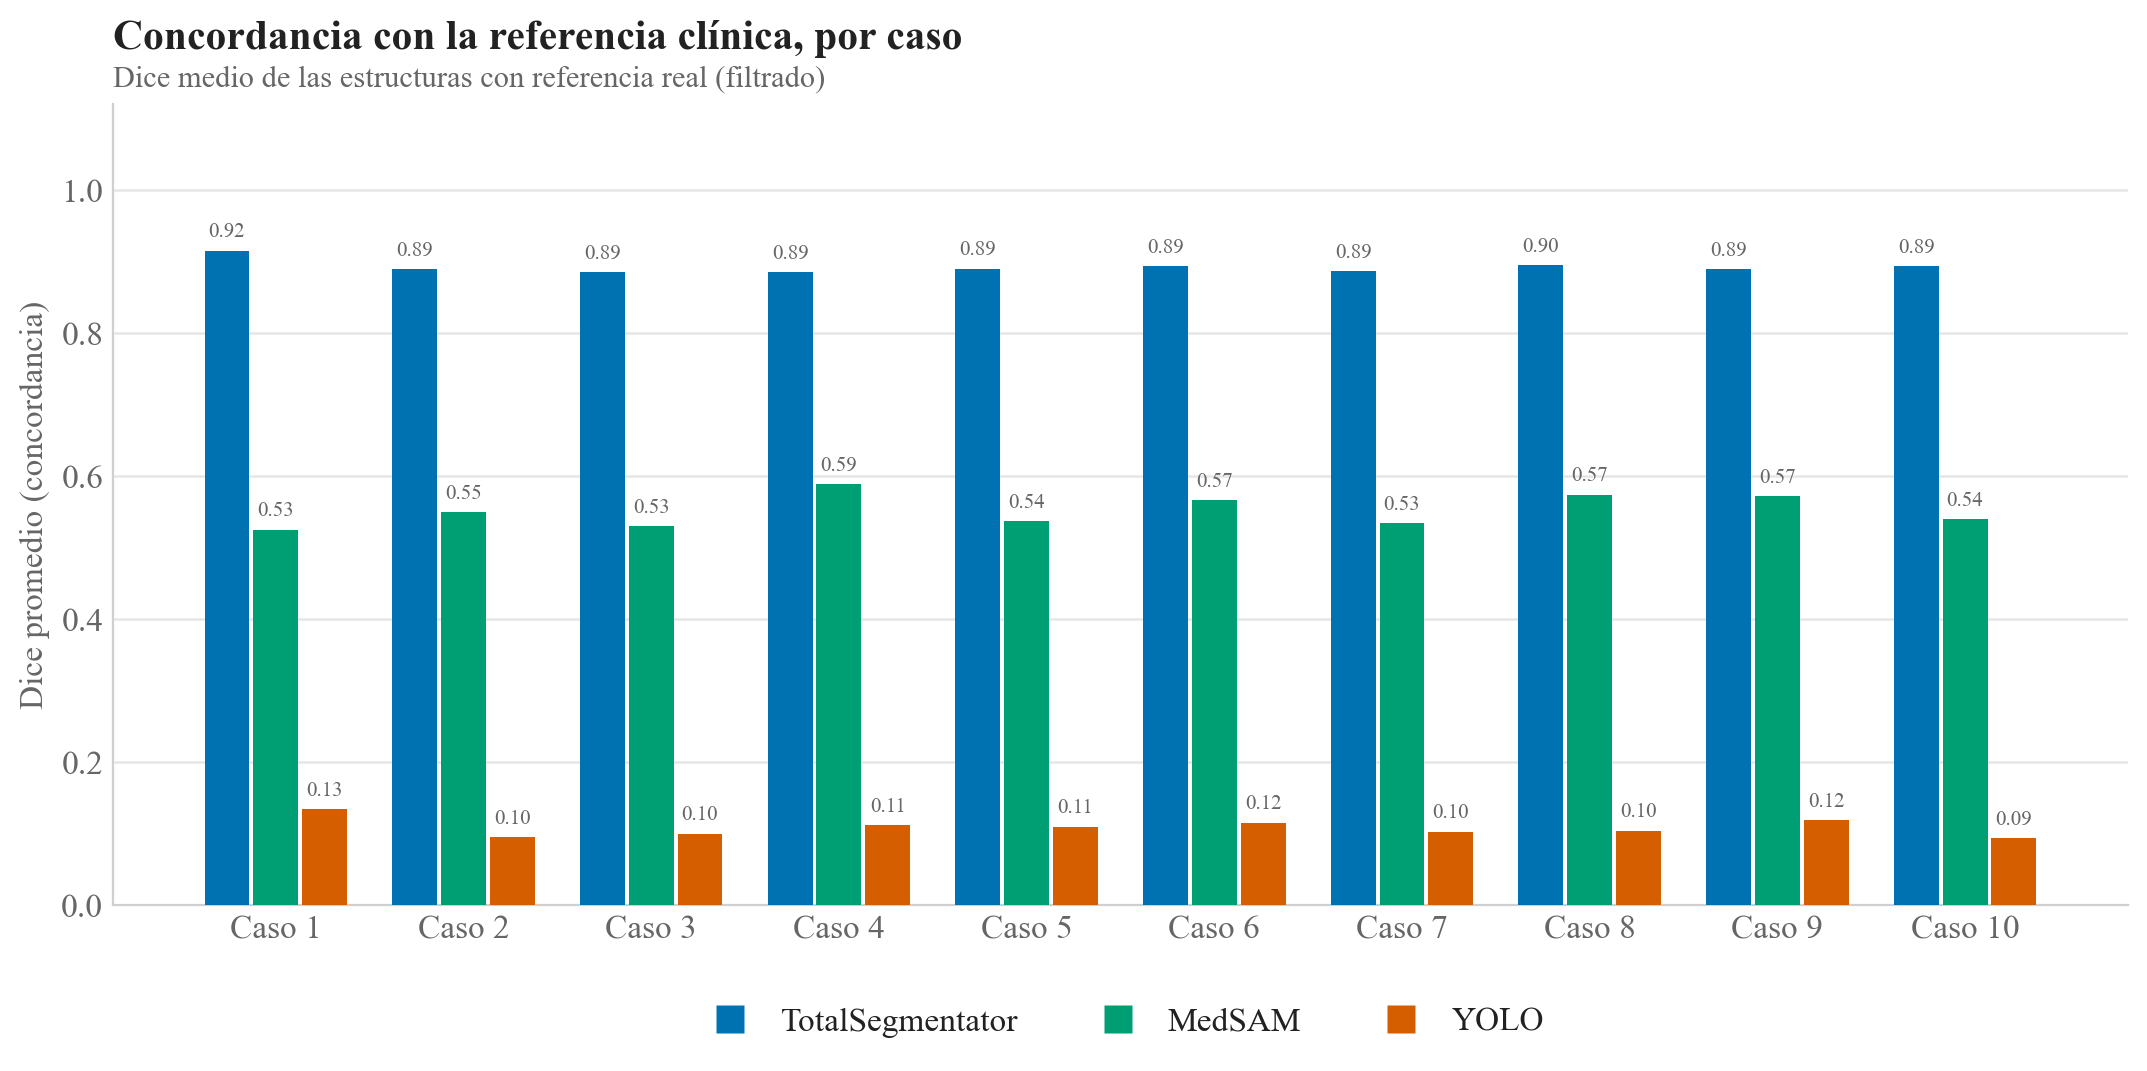
\includegraphics[width=0.9\textwidth]{graficos/1_dice_por_caso.png}
  \caption{Concordancia con la referencia clínica por caso, medida como coeficiente de Dice promedio sobre las estructuras con referencia no vacía.}
  \label{fig:dice-por-caso}
  \begin{minipage}{\textwidth}
    \centering
    \normalsize Fuente: Elaboración propia.\\
  \end{minipage}
\end{figure}

Desglosada por región anatómica (Figura~\ref{fig:radar-categorias}), la concordancia de TotalSegmentator es alta y uniforme en todas las categorías, en tanto que la de MedSAM cae en las estructuras óseas y de vía aérea, y la de YOLO se limita a las regiones de gran volumen.\\

\begin{figure}[H]
  \centering
  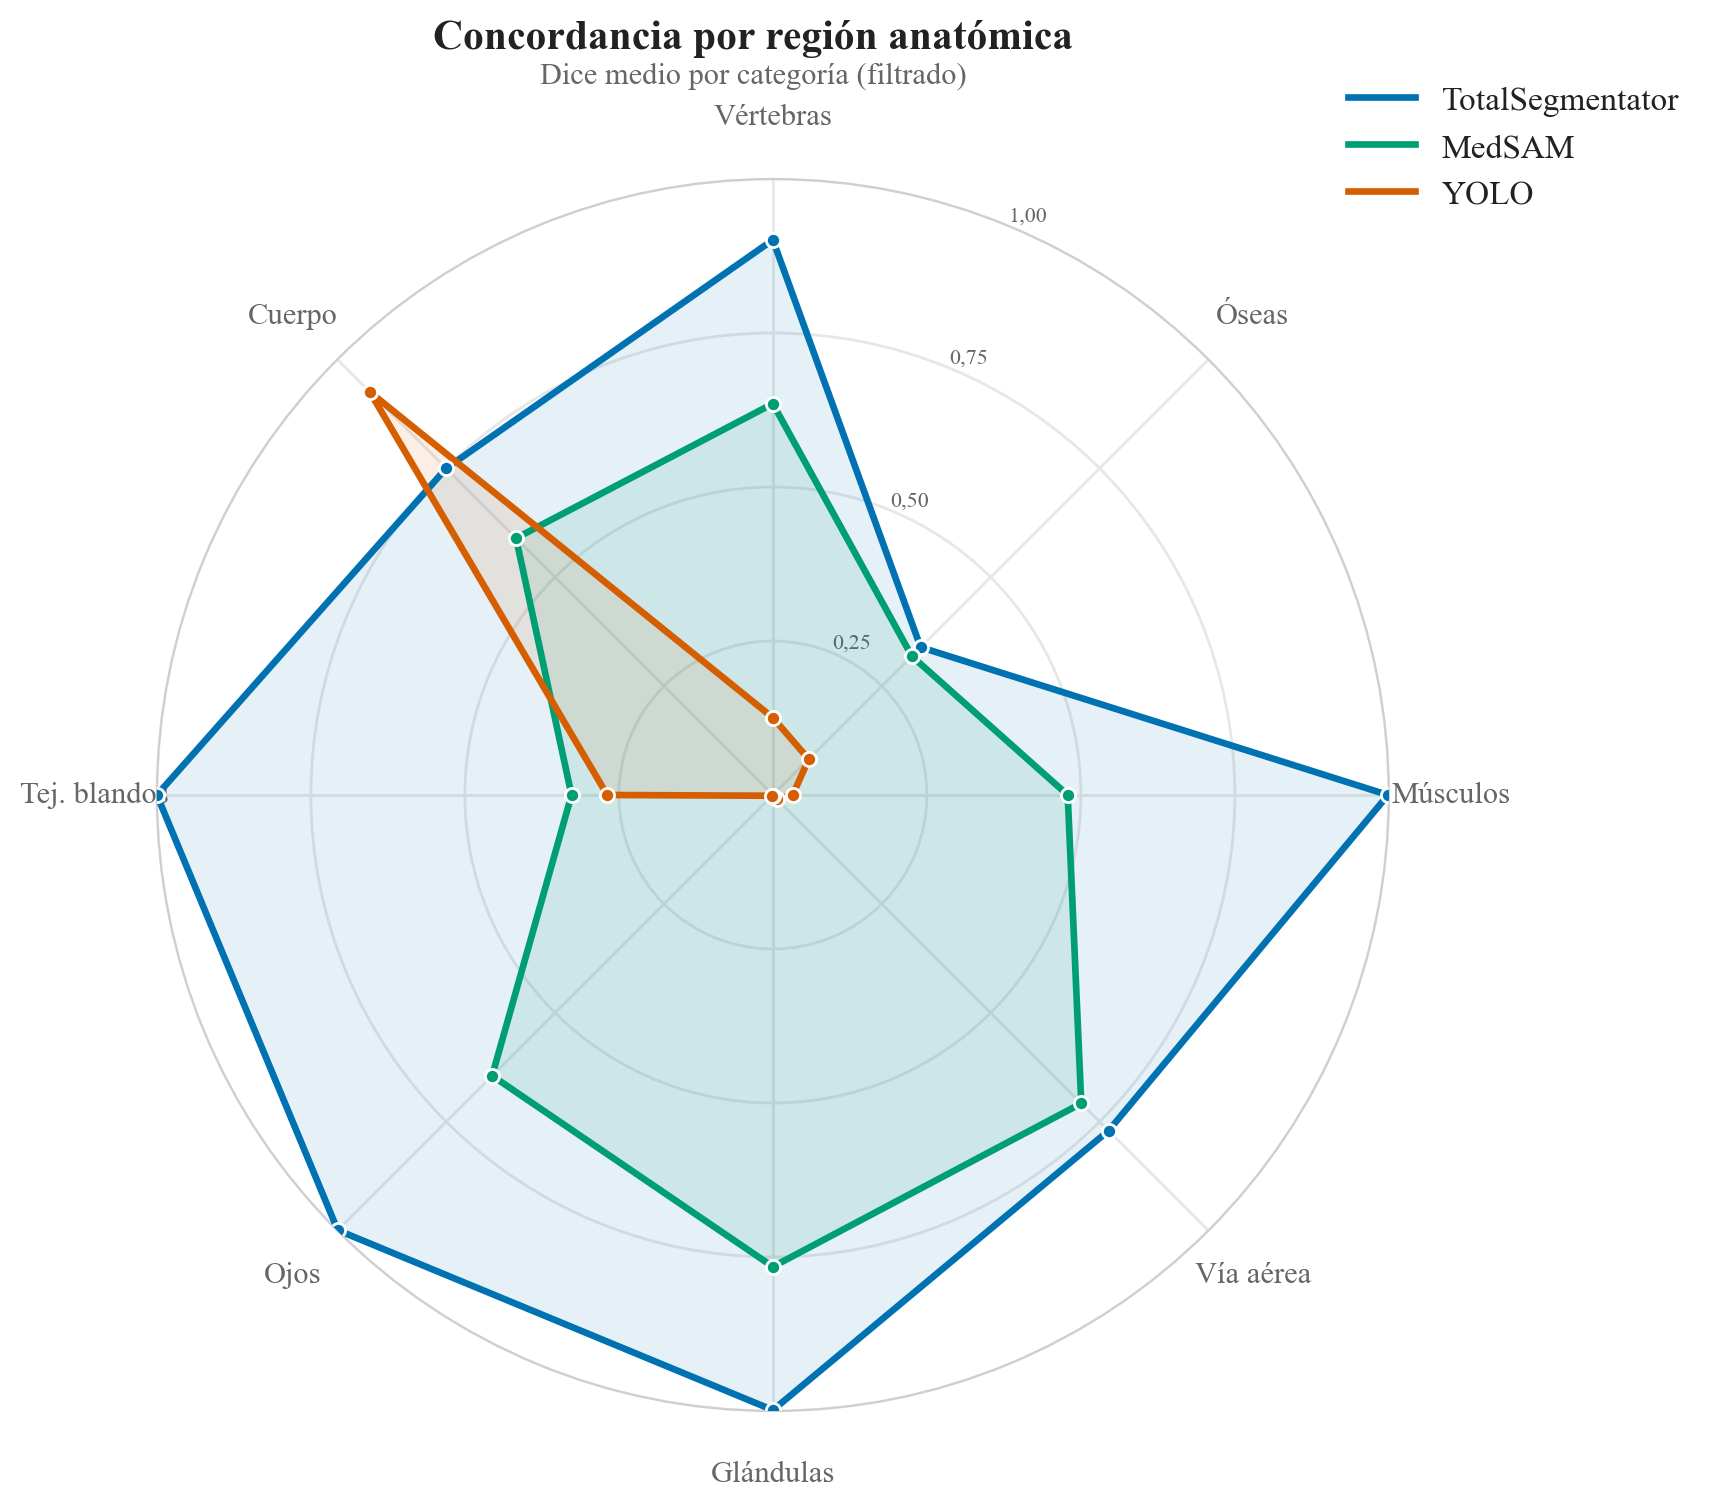
\includegraphics[width=0.72\textwidth]{graficos/2_radar_categorias.png}
  \caption{Concordancia por región anatómica. Cada eje representa una categoría de estructuras, con el Dice promedio de los diez casos.}
  \label{fig:radar-categorias}
  \begin{minipage}{\textwidth}
    \centering
    \normalsize Fuente: Elaboración propia.\\
  \end{minipage}
\end{figure}

La Figura~\ref{fig:niveles-calidad} resume, para cada modelo, cuántas de las 64 estructuras de la referencia alcanzan cada nivel de concordancia. TotalSegmentator concentra la mayoría en los niveles altos; MedSAM se reparte entre niveles medios y bajos; YOLO acumula casi todas sus estructuras en el nivel nulo.\\

\begin{figure}[H]
  \centering
  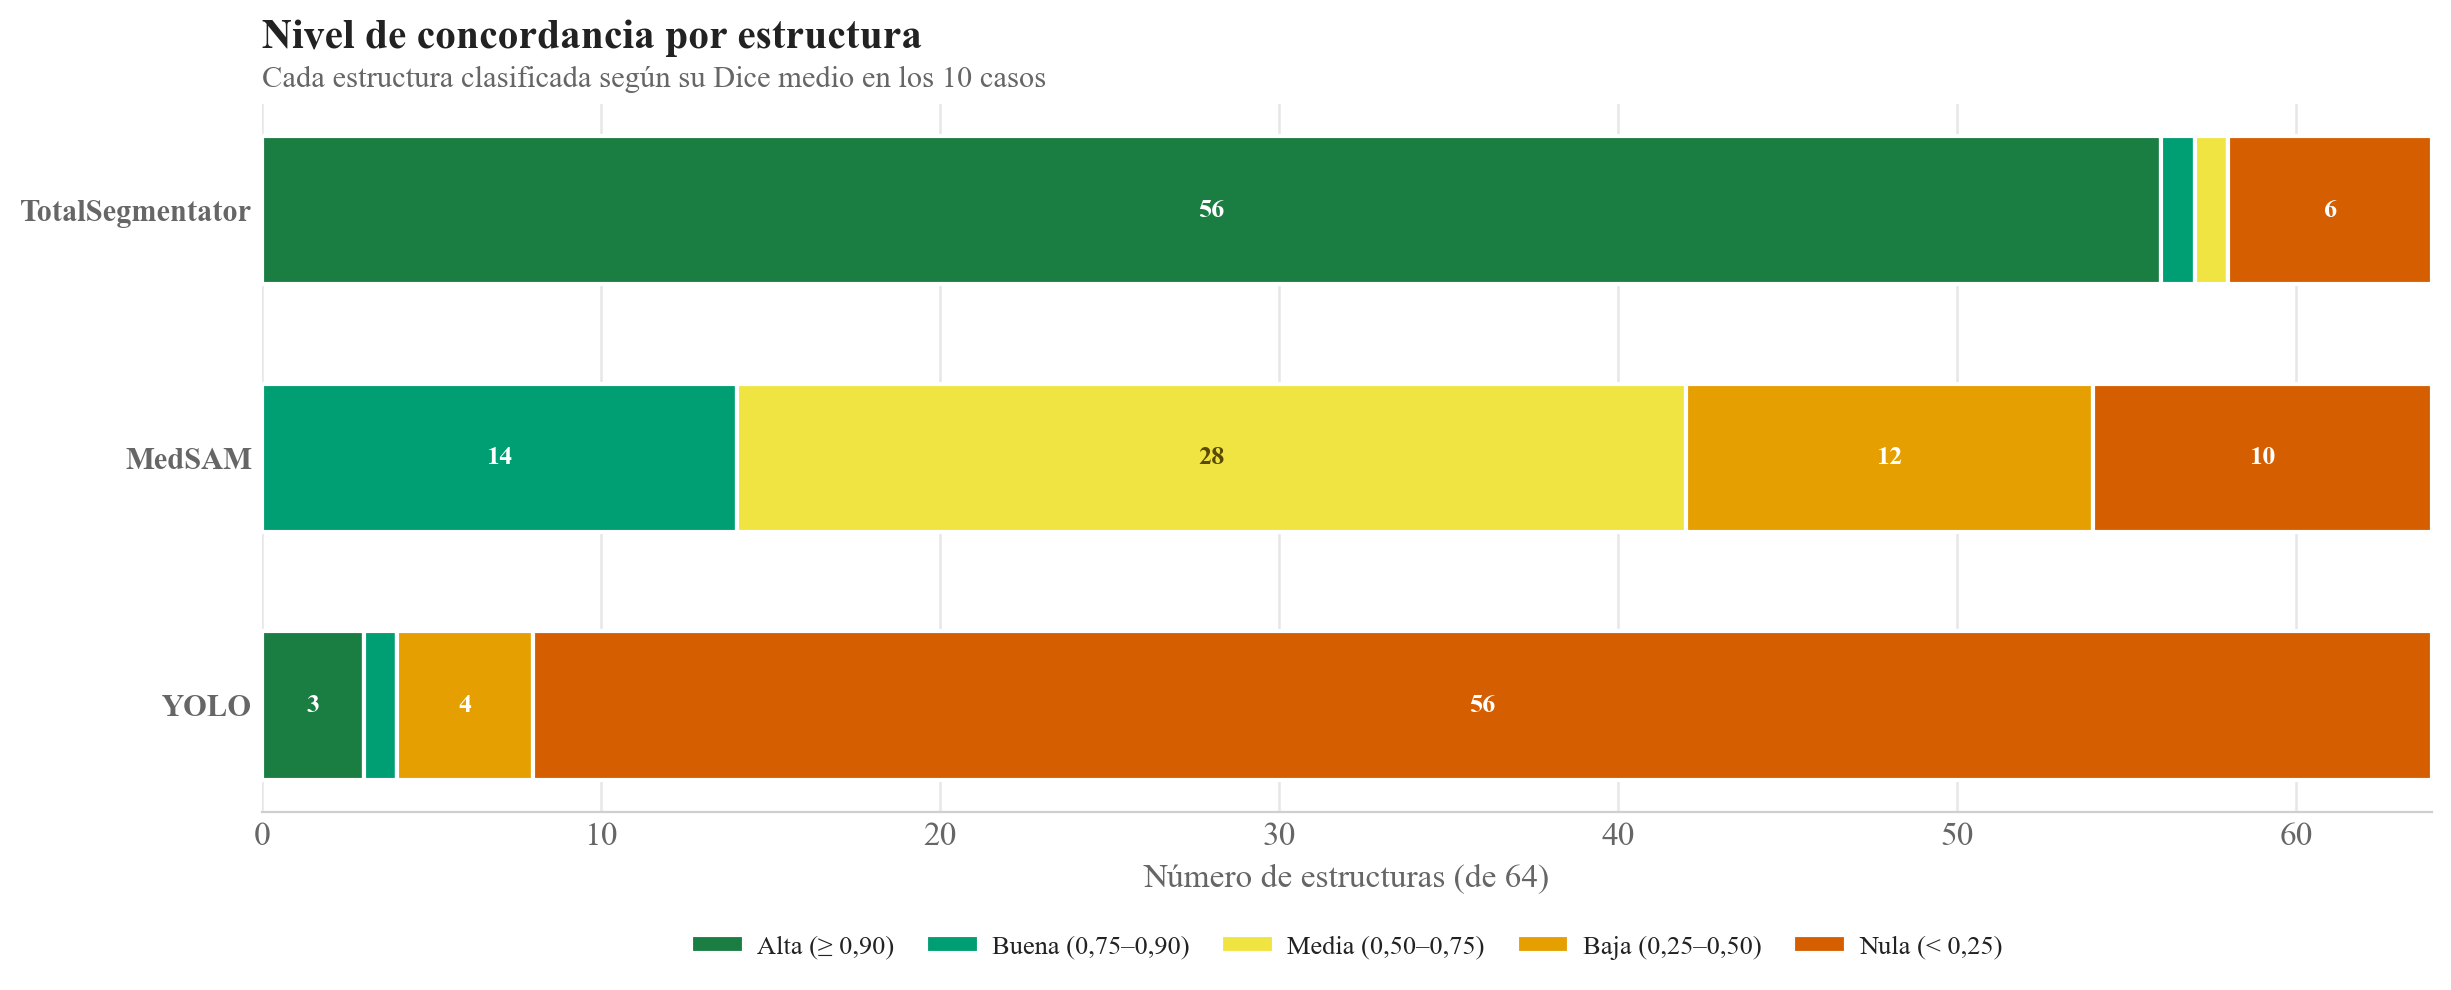
\includegraphics[width=0.95\textwidth]{graficos/3_niveles_calidad.png}
  \caption{Nivel de concordancia por estructura. Cada estructura de la referencia se clasifica según su Dice medio en los diez casos.}
  \label{fig:niveles-calidad}
  \begin{minipage}{\textwidth}
    \centering
    \normalsize Fuente: Elaboración propia.\\
  \end{minipage}
\end{figure}

\subsection{Sensibilidad al umbral de detección}

La cobertura anterior depende del umbral de Dice que se exija para dar una estructura por detectada. Para verificar que la comparación no descansa en un umbral arbitrario, la Tabla~\ref{tab:sensibilidad} reporta la cobertura de cada modelo en tres umbrales: 0,3, 0,5 y 0,667, este último equivalente a una intersección sobre la unión de 0,5, criterio estándar de detección \citep{everingham2010pascal}.\\

\begin{table}[H]
  \centering
  \caption{Cobertura efectiva de cada modelo según el umbral de Dice exigido.}
  \label{tab:sensibilidad}
  \begin{tabular}{lccc}
    \hline
    \textbf{Modelo} & \textbf{Dice $\geq$ 0,3} & \textbf{Dice $\geq$ 0,5} & \textbf{Dice $\geq$ 0,667} \\
    \hline
    TotalSegmentator & 90,8\% & 90,8\% & 90,8\% \\
    MedSAM           & 81,4\% & 64,6\% & 36,1\% \\
    YOLOv8x-seg      & 13,4\% & 7,6\%  & 6,3\%  \\
    \hline
  \end{tabular}
  \begin{minipage}{\textwidth}
    \centering
    \normalsize Fuente: Elaboración propia.\\
  \end{minipage}
\end{table}

La cobertura de TotalSegmentator no varía entre umbrales: las estructuras que segmenta superan incluso el criterio más estricto, sin acumular resultados de calidad marginal. MedSAM pierde más de la mitad de su cobertura al pasar de 0,3 a 0,667, lo que revela que buena parte de las estructuras que aparentaba cubrir lo hacía con segmentaciones deficientes. YOLO se mantiene bajo en todos los umbrales. Las siete estructuras que este último supera de forma consistente son el contorno corporal (\texttt{body}, \texttt{body\_trunc}, \texttt{body\_extremities}, \texttt{head}), la piel, la grasa subcutánea y el músculo esquelético como masa global: todas envolturas externas o regiones de gran volumen y alto contraste. YOLO no segmenta de forma fiable ninguna estructura anatómica interna, que son justamente las que un fantoma de cricotiroidotomía necesita.\\

\begin{figure}[H]
  \centering
  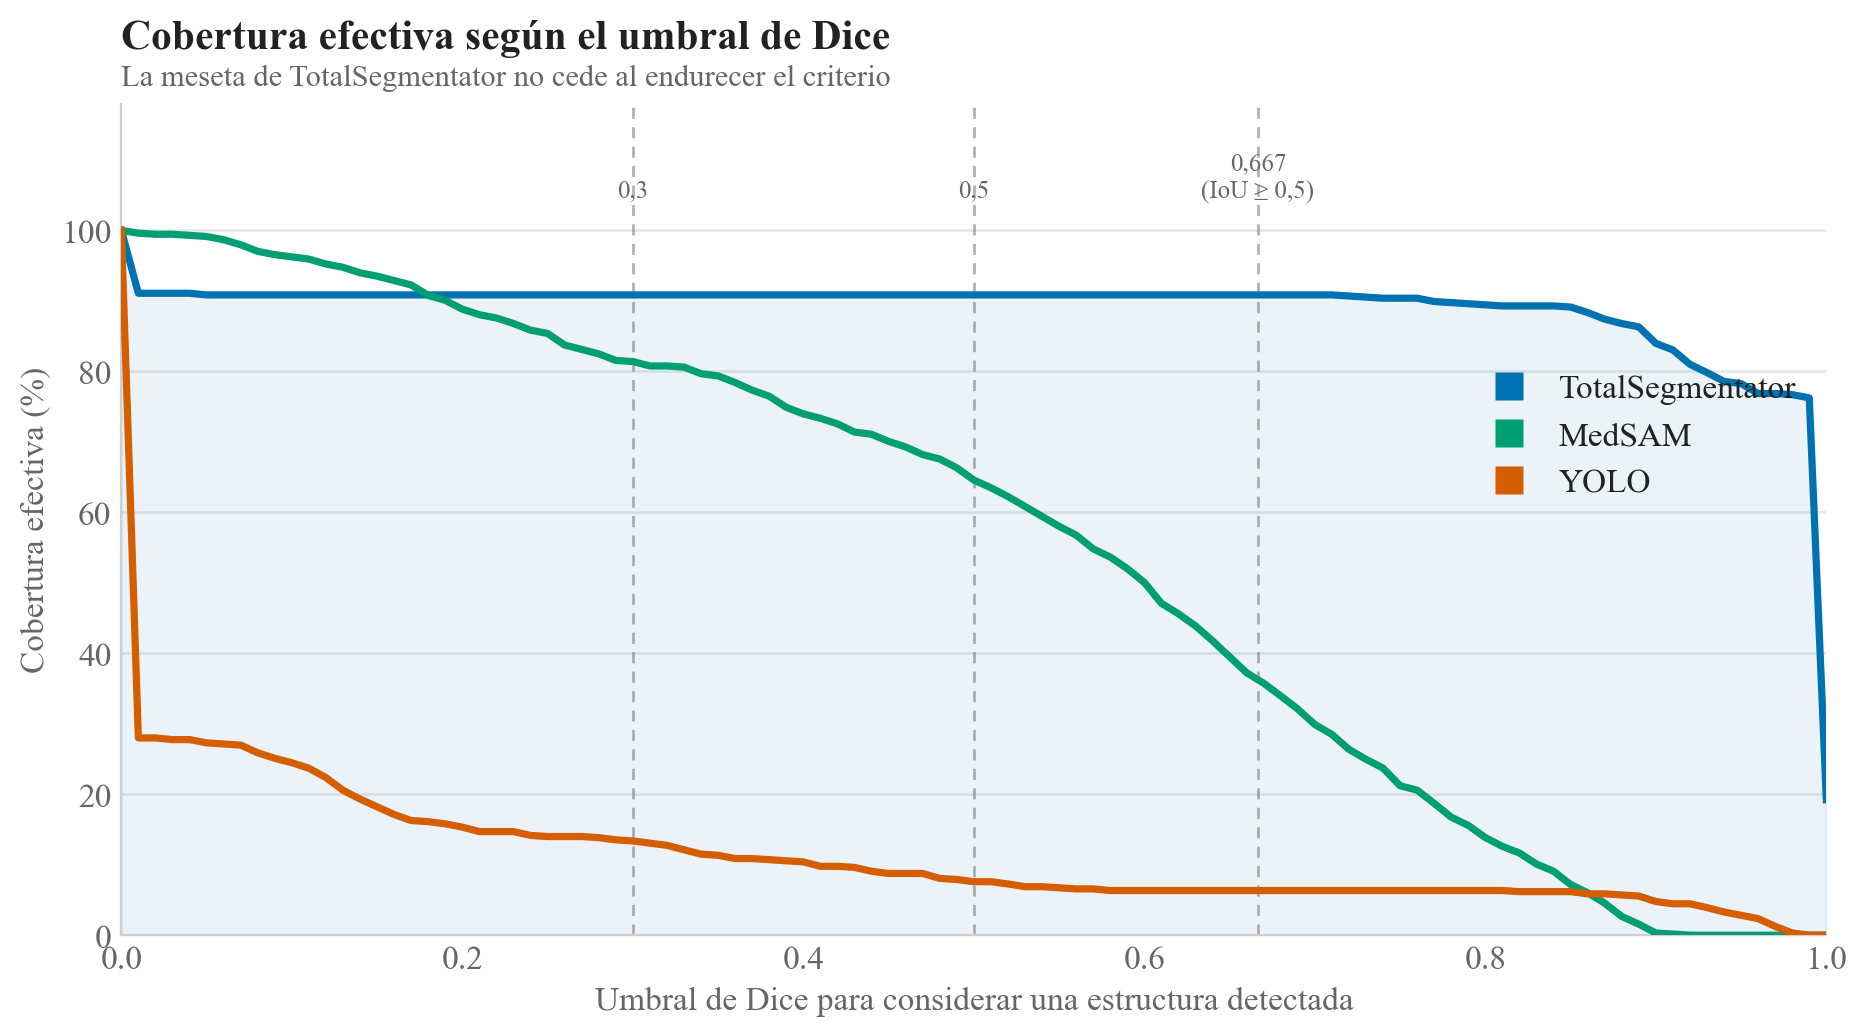
\includegraphics[width=0.9\textwidth]{graficos/5_sensibilidad_umbral.png}
  \caption{Cobertura de cada modelo en función del umbral de Dice exigido. Las líneas verticales marcan los tres umbrales de la Tabla~\ref{tab:sensibilidad}.}
  \label{fig:sensibilidad}
  \begin{minipage}{\textwidth}
    \centering
    \normalsize Fuente: Elaboración propia.\\
  \end{minipage}
\end{figure}

Estos resultados son coherentes con la naturaleza de cada modelo. YOLO fue concebido para detección bidimensional en imágenes naturales y se evaluó procesando la TC corte a corte, una tarea para la que no fue diseñado. MedSAM, aunque especializado en imágenes médicas, depende de indicaciones que en un flujo autónomo no están disponibles, y mostró dificultades en estructuras finas o de bajo contraste. TotalSegmentator está entrenado específicamente para segmentación volumétrica multiclase sobre TC.\\

La Figura~\ref{fig:tiempo-cobertura} cruza las dos dimensiones que importan para el sistema: la cobertura efectiva y el tiempo de inferencia. TotalSegmentator ocupa la región de interés, con cobertura alta y tiempo moderado; MedSAM alcanza un tiempo similar con menor cobertura; YOLO es el más rápido pero con cobertura casi nula, lo que lo descarta pese a su velocidad.\\

\begin{figure}[H]
  \centering
  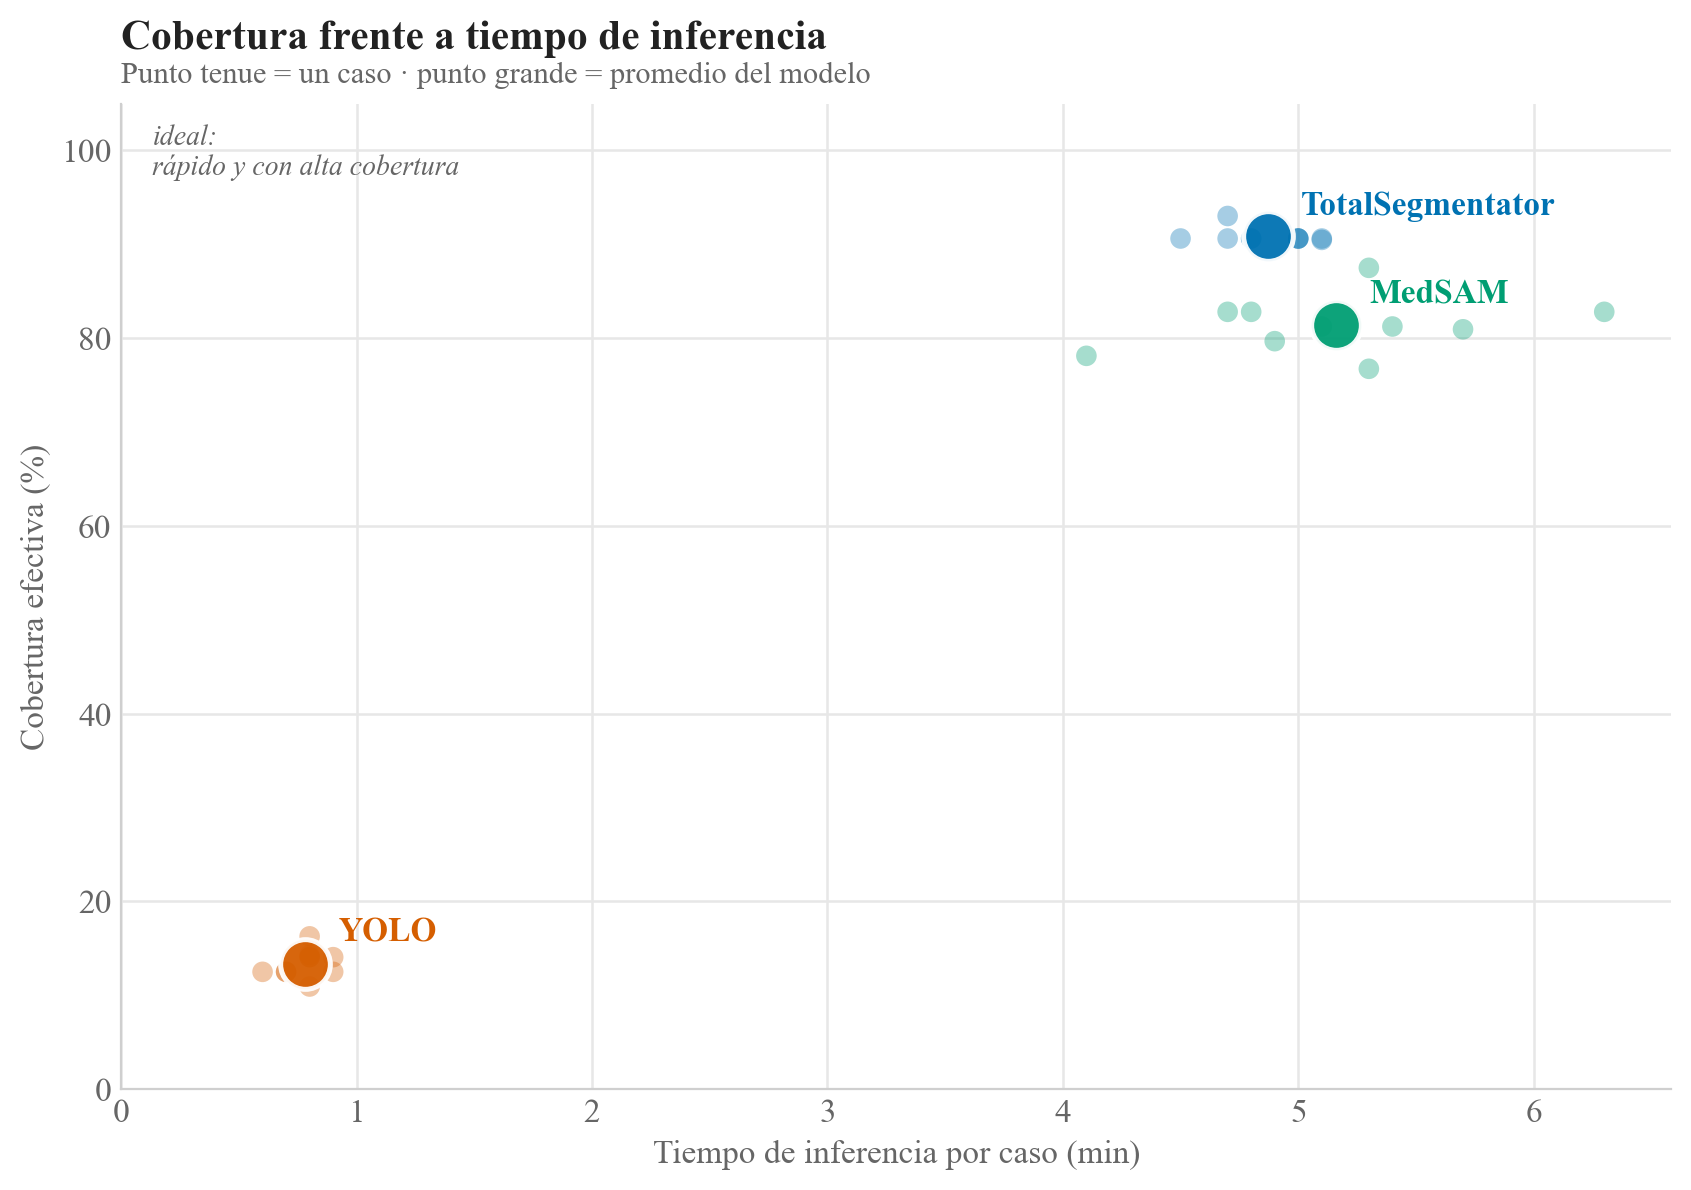
\includegraphics[width=0.82\textwidth]{graficos/6_tiempo_vs_cobertura.png}
  \caption{Cobertura efectiva frente a tiempo de inferencia. Cada punto tenue es un caso; el punto grande, el promedio de cada modelo.}
  \label{fig:tiempo-cobertura}
  \begin{minipage}{\textwidth}
    \centering
    \normalsize Fuente: Elaboración propia.\\
  \end{minipage}
\end{figure}

\subsection{Fundamento de la selección del motor de segmentación}

Dado que las métricas de superposición no pueden arbitrar de forma imparcial, la selección de TotalSegmentator se sostiene sobre criterios independientes de ellas.\\

\begin{enumerate}
  \item \textbf{Autonomía.} Es el único de los tres modelos capaz de segmentar sin indicaciones manuales por estructura. MedSAM requiere recuadros delimitadores que, en un uso real, solo podrían provenir de una segmentación previa, lo que anula el propósito del sistema. YOLO opera sin indicaciones, pero no segmenta ninguna estructura anatómica interna. Este criterio, por sí solo, descarta ambas alternativas.

  \item \textbf{Validación clínica implícita.} El radiólogo del proyecto, sin intervención del equipo, eligió TotalSegmentator como punto de partida para elaborar la referencia y aceptó su salida sin modificaciones en la mayoría de las estructuras, con correcciones circunscritas a las vértebras cervicales y la tráquea. Se trata de una validación por parte de un especialista, independiente de cualquier métrica calculada por los autores.

  \item \textbf{Estructuras del punto de incisión.} TotalSegmentator es el único que produce el cartílago tiroides, el cricoides, el hioides y la laringe, que delimitan la membrana cricotiroidea y dan sentido al fantoma.

  \item \textbf{Tiempo de procesamiento.} Segmenta un caso completo en torno a cinco minutos, un costo compatible con el uso operativo del sistema.
\end{enumerate}

Los cuatro criterios apuntan en la misma dirección y ninguno se apoya en la comparación contra la referencia. La elección se habría mantenido aun descartando por completo las métricas de superposición.\\

\subsection{Cobertura anatómica del sistema integrado}

Integrado en el flujo, el sistema produce 58 de las 64 estructuras que contiene la referencia. Las seis restantes se concentran en la región craneofacial: la mandíbula (\texttt{mandible}), las dos arcadas dentarias (\texttt{teeth\_upper}, \texttt{teeth\_lower}), los senos frontal y maxilar (\texttt{sinus\_ frontal}, \texttt{sinus\_maxillary}) y la estructura global de cabeza (\texttt{head}). Estas seis provienen de una tarea de TotalSegmentator no incluida en la configuración actual, orientada específicamente a la región de interés del proyecto.\\

Estas cifras se entienden mejor desde el objetivo del sistema que desde la referencia. El sistema no busca reproducir las 64 estructuras de la referencia, sino producir un modelo anatómico útil para la región de cabeza y cuello, y bajo ese objetivo la cifra relevante no es 58 de 64, sino 121: el número de estructuras con contenido real que el flujo conserva y entrega para un caso cervical, casi el doble de las que contiene la referencia. Entre ellas están las cuatro que delimitan el punto de incisión de la cricotiroidotomía (cartílago tiroides, cricoides, hioides y laringe), que la referencia del radiólogo ni siquiera incluye. El sistema demuestra así que, con la configuración de tareas adecuada, es capaz de generar una zona anatómica considerablemente más detallada que la referencia de comparación.\\

Esa amplitud, sin embargo, no llega directamente al fantoma final. El módulo de corte, descrito en el Capítulo~\ref{ch:diseno-del-producto}, permite al usuario recortar el modelo hasta la región de interés antes de exportar, con lo que las 121 estructuras generadas se reducen a las que efectivamente se necesitan imprimir para el procedimiento. La generación exhaustiva y el recorte selectivo quedan así como dos etapas separadas: primero segmentar todo lo que la imagen permite, y luego decidir qué imprimir, en lugar de decidir de antemano qué segmentar.\\

Concordancia y cobertura miden aspectos distintos y conviene no confundirlas. La Figura~\ref{fig:dice-por-caso} muestra qué tan bien se superpone lo que cada modelo segmenta; la Figura~\ref{fig:cobertura-efectiva}, qué proporción de las estructuras de referencia alcanza a segmentar. Un modelo podría concordar muy bien en las pocas estructuras que detecta y aun así cubrir pocas, de modo que ambas se reportan por separado.\\

\begin{figure}[H]
  \centering
  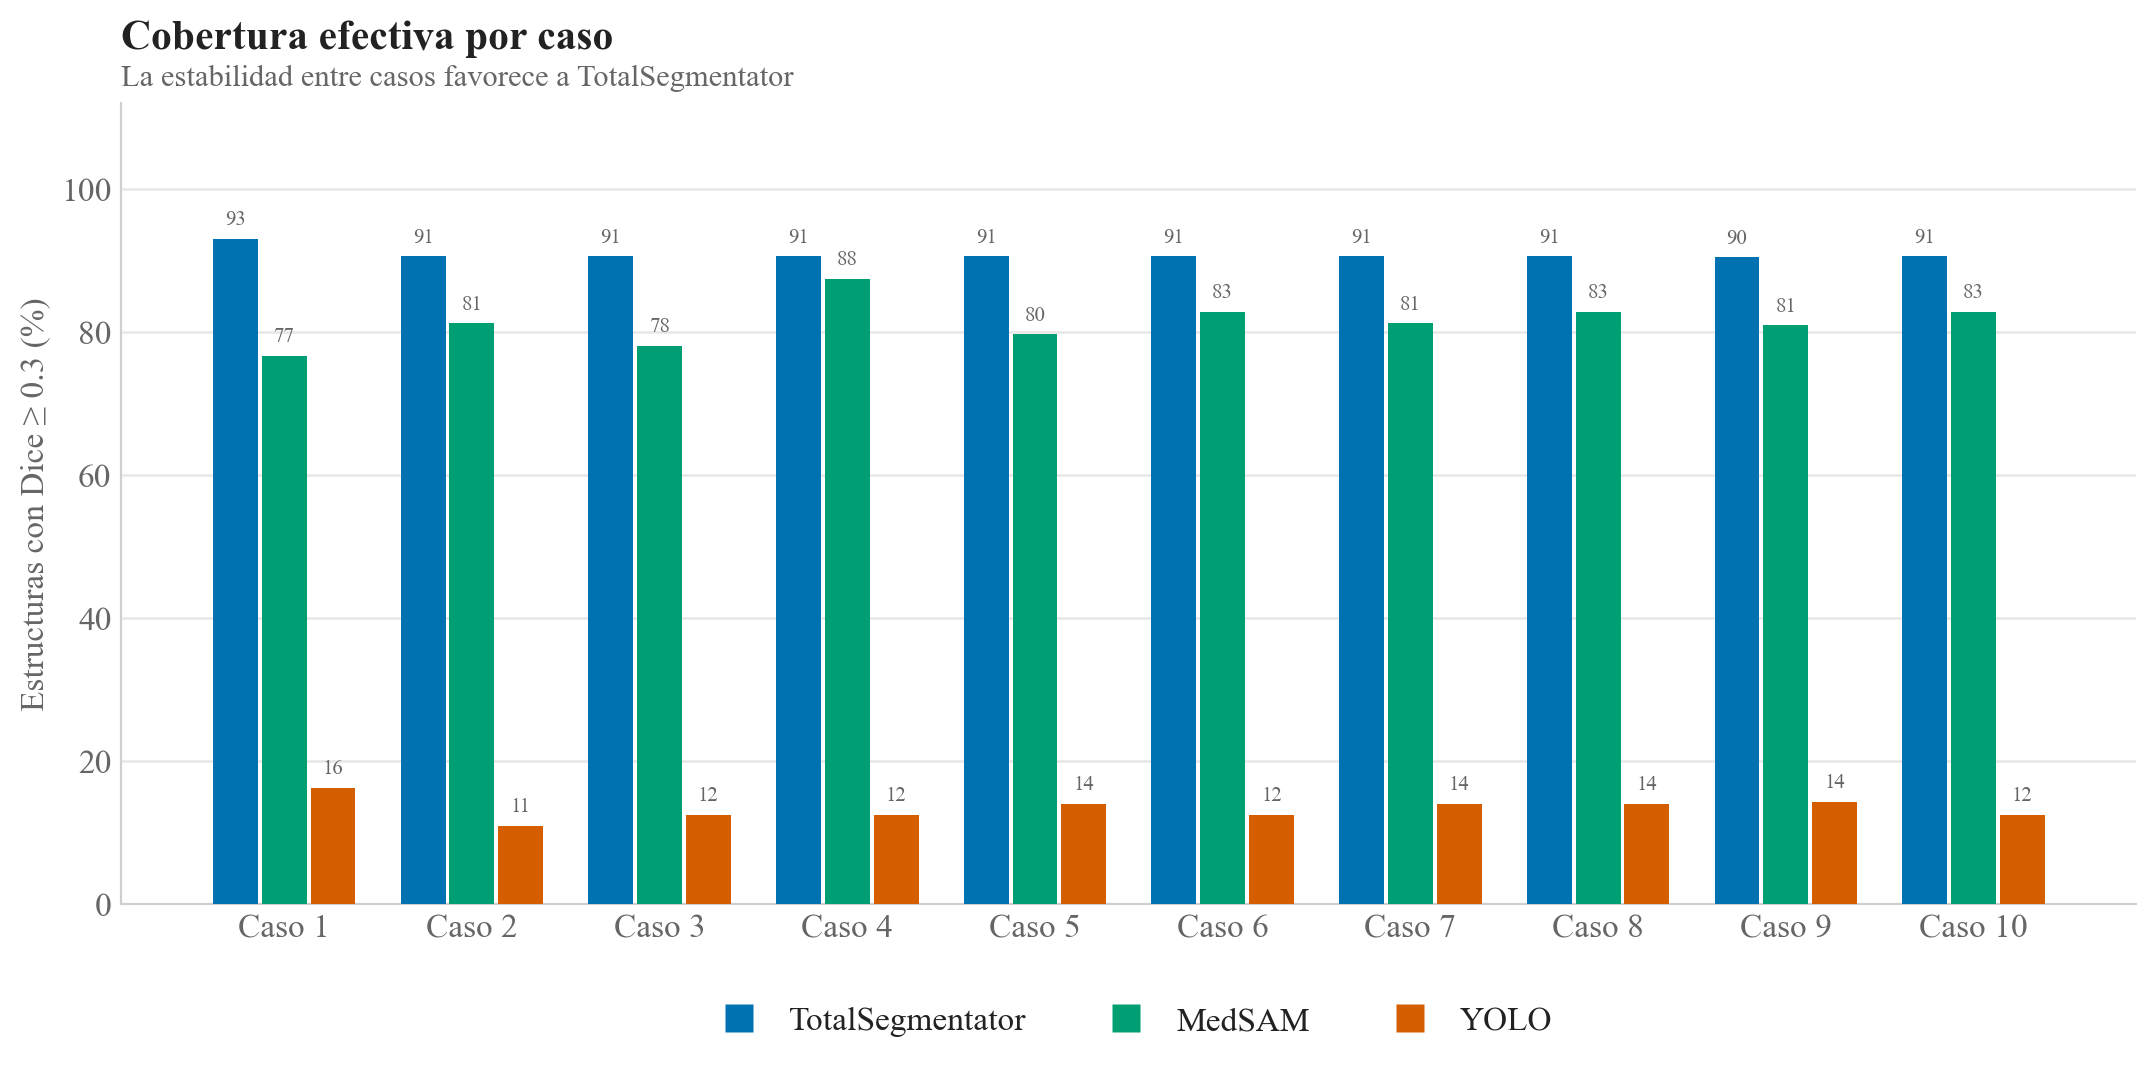
\includegraphics[width=0.9\textwidth]{graficos/4_cobertura_por_caso.png}
  \caption{Cobertura efectiva por caso y modelo, calculada sobre las estructuras con referencia no vacía en cada caso. La estabilidad entre casos favorece a TotalSegmentator.}
  \label{fig:cobertura-efectiva}
  \begin{minipage}{\textwidth}
    \centering
    \normalsize Fuente: Elaboración propia.\\
  \end{minipage}
\end{figure}

\subsection{Generalización a otras regiones anatómicas}

Aunque el sistema fue configurado para la región cervical, su arquitectura no está atada a ella. Para verificarlo se procesó una TC de pie a través del módulo completo, sin modificar el código ni la configuración. El flujo ejecutó sus cuatro etapas sin intervención, segmentó las estructuras presentes en el volumen y generó los archivos STL correspondientes. Esto confirma que el recorrido (preprocesamiento, segmentación remota, consolidación por filtro espacial, corte y exportación) es independiente de la anatomía de entrada, lo que se explica por el criterio de consolidación adoptado: al conservar toda máscara con contenido real en lugar de contrastarla contra una lista fija de nombres, el sistema no presupone qué estructuras debería encontrar. Lo que sí depende de la región es el conjunto de tareas de TotalSegmentator que se ejecuta, hoy orientado a cabeza y cuello, de modo que la cobertura alcanzable en otras zonas es menor que la posible. Esta limitación se recoge entre las mejoras propuestas.\\

\begin{figure}[H]
  \centering
  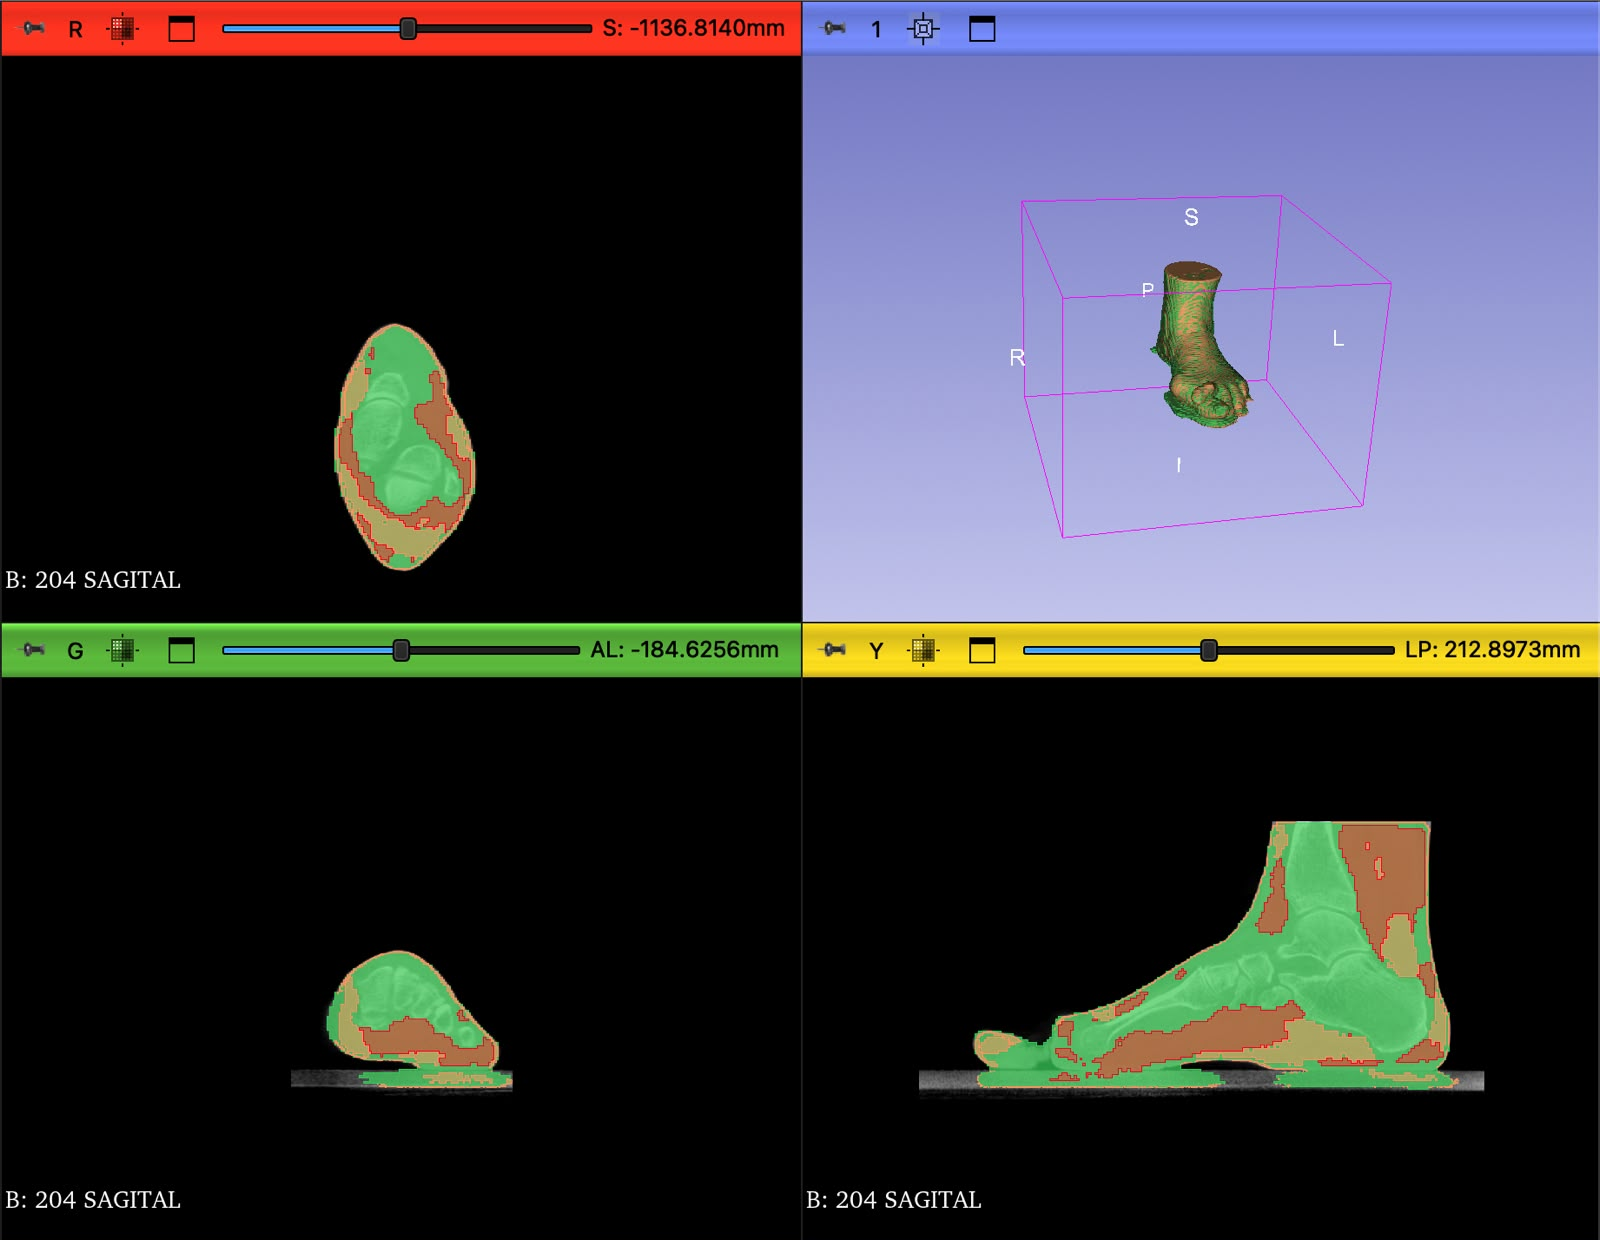
\includegraphics[width=0.9\textwidth]{imagenes/pie-segmentado.jpeg}
  \caption{Generalización del flujo a una TC de pie, procesada a través del módulo completo sin modificar el código ni la configuración.}
  \label{fig:pie-segmentado}
  \begin{minipage}{\textwidth}
    \centering
    \normalsize Fuente: Elaboración propia.\\
  \end{minipage}
\end{figure}

\subsection{Tiempo de procesamiento}

Los tiempos de la Tabla~\ref{tab:comparacion} corresponden únicamente a la inferencia de cada modelo, que es la magnitud comparable entre las tres herramientas. El tiempo que percibe el usuario es distinto y mayor, ya que la inferencia es solo una de las etapas que ejecuta el módulo. La Tabla~\ref{tab:tiempos-etapa} desglosa una ejecución completa sobre un caso de TC cervical.\\

\begin{table}[H]
  \centering
  \caption{Desglose del tiempo de una ejecución completa del módulo de segmentación, en modo remoto.}
  \label{tab:tiempos-etapa}
  \begin{tabular}{lcc}
    \hline
    \textbf{Etapa} & \textbf{Tiempo} & \textbf{Proporción} \\
    \hline
    Preprocesamiento de la TC & \tPreproc  & 14\% \\
    Envío de la TC al servidor & \tEnvio   & 3\%  \\
    Segmentación en GPU & \tSeg            & 18\% \\
    Recuperación y escritura local de las estructuras & \tLocal & 54\% \\
    Limpieza de archivos en el servidor & \tLimpieza & 11\% \\
    \hline
    \textbf{Total} & \textbf{\tTotal} & \textbf{100\%} \\
    \hline
  \end{tabular}
  \begin{minipage}{\textwidth}
    \centering
    \normalsize Fuente: Elaboración propia.\\
  \end{minipage}
\end{table}

El proceso completo toma cerca de \tTotal{} por caso, por debajo del límite de 30 minutos fijado en los requisitos, aunque sin holgura. El desglose muestra algo que no era evidente de antemano: la segmentación, que es la etapa computacionalmente exigente y la que motivó toda la infraestructura remota, representa una fracción menor del tiempo total. La mayor parte se consume en la recuperación y el manejo local de las estructuras segmentadas, no en el cómputo ni en la transferencia por la red.\\

La razón es el volumen de archivos. El sistema conserva más de cien estructuras con contenido, cada una en un archivo NIfTI independiente, que deben escribirse y procesarse en el equipo local. El costo no está en el tamaño total ni en la red, sino en la cantidad de operaciones de entrada y salida sobre muchos archivos. El preprocesamiento y la limpieza remota responden a una situación análoga: son operaciones sobre archivos, no de cálculo.\\

La conclusión operativa es que el sistema no está limitado por su capacidad de cómputo sino por su manejo de archivos, y las mejoras de tiempo más rentables no pasan por una GPU más potente. Esta línea se retoma en la sección de mejoras.\\

\subsection{Cumplimiento de los criterios definidos}

Los resultados anteriores permiten contrastar el sistema con los criterios enunciados en el Capítulo~\ref{ch:solucion-planteada}. El criterio de autonomía se cumple: el motor seleccionado segmenta sin requerir indicaciones manuales por estructura, lo que hace posible el flujo automatizado. El criterio de cobertura de las estructuras del procedimiento también se cumple: el sistema produce el cartílago tiroides, el cricoides, el hioides, la laringe y la tráquea, que delimitan la región de la maniobra. El requisito de tiempo, fijado en un máximo de 30 minutos por caso, se satisface con \tTotal{}. Los archivos STL producidos se cargan en el laminador sin requerir reparación previa de la malla. Los criterios de usabilidad y portabilidad se satisfacen por construcción, aunque la usabilidad no ha sido verificada con usuarios clínicos, lo que constituye la limitación principal del trabajo.\\

La Tabla~\ref{tab:cumplimiento} sintetiza el estado de cada requisito definido en el Capítulo~\ref{ch:solucion-planteada}.\\

\begin{table}[H]
  \centering
  \caption{Cumplimiento de los requisitos. Fuente: Elaboración propia.}
  \label{tab:cumplimiento}
  \small
  \begin{tabular}{p{1.1cm} p{8.6cm} p{2.4cm}}
    \hline
    \textbf{ID} & \textbf{Requisito} & \textbf{Estado} \\
    \hline
    RF1 & Ingreso de la TC en NIfTI, anonimizado & Cumple \\
    RF2 & Segmentación automática remota sobre GPU & Cumple \\
    RF3 & Consolidación independiente de la imagen & Cumple \\
    RF4 & Visualización 3D en Slicer & Cumple \\
    RF5 & Corte y reorientación con planos & Cumple \\
    RF6 & Exportación a STL con color por tejido & Cumple \\
    RO1 & Operación sin GPU local & Cumple \\
    RO2 & STL imprimibles sin reparación & Cumple \\
    RO3 & Tiempo por caso $\leq$ 30 min & Cumple \\
    RO4 & Costo de material reducido & Cumple \\
    CC1 & Autonomía (eliminatorio) & Cumple \\
    CC2 & Cobertura de las estructuras del procedimiento & Cumple \\
    CC3 & Usabilidad & Parcial \\
    CC4 & Portabilidad & Cumple \\
    CC5 & Escalabilidad a otras regiones & Cumple \\
    \hline
  \end{tabular}
  \begin{minipage}{\textwidth}
    \centering
    \normalsize Fuente: Elaboración propia.\\
  \end{minipage}
\end{table}

El único requisito con cumplimiento parcial es la usabilidad (CC3): se satisface por construcción, pero no ha sido verificada con usuarios clínicos, lo que constituye la limitación principal del trabajo.\\

\subsection{Generación del modelo imprimible}

Como resultado del flujo completo, el sistema produce, a partir de una TC cervical, un conjunto de archivos STL (uno por estructura anatómica) centrados, orientados y cerrados, aptos para cargarse en un laminador e imprimirse sin correcciones previas. El recorrido que va desde la imagen médica hasta el modelo imprimible queda así cubierto de forma automatizada y operable por personal sin formación en procesamiento de imágenes.\\

Sobre esa base, y de forma opcional, los modelos admiten un paso adicional de optimización en el laminador. La simplificación de la malla, que reduce el número de polígonos aproximadamente a la mitad, aligera el archivo y mejora la calidad del laminado sin pérdida perceptible de detalle anatómico. Este ajuste se realizó manualmente en las impresiones efectuadas y, si bien no es condición necesaria para imprimir, incorporarlo al propio módulo mejoraría el resultado de forma automática.\\

Los archivos STL producidos se cargan en el laminador e imprimen sin requerir reparación previa de la malla. Dicho esto, es recomendable inspeccionarlos antes de imprimir, para verificar la ausencia de fragmentos flotantes o polígonos mal formados, y simplificar la malla, lo que mejora la calidad del laminado. El sistema no elimina esa revisión, pero reduce la preparación a una inspección visual en lugar de una reconstrucción de la geometría.\\

\subsection{Fantoma físico impreso}
 
El recorrido completo se validó materialmente mediante la impresión de fantomas a partir de los archivos generados por el sistema, lo que confirma que el flujo entrega un objeto físico coherente con la TC de entrada. La fabricación no fue inmediata: atravesó cuatro generaciones sucesivas, cada una motivada por las limitaciones de la anterior, hasta llegar a un resultado a color que expone las estructuras internas del cuello.\\
 
La primera generación se imprimió estructura por estructura, en piezas separadas que luego se ensamblaron manualmente con adhesivo. El enfoque resultó frágil y laborioso: el ensamblado de decenas de piezas pequeñas es propenso a errores de posición y consume un tiempo considerable, además de que las estructuras finas presentaban fragmentos sueltos y baja adherencia.\\
 
\begin{figure}[H]
  \centering
  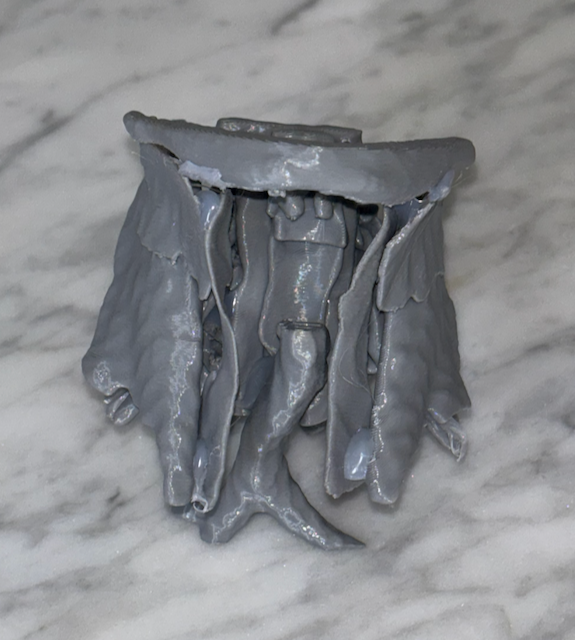
\includegraphics[width=0.46\textwidth]{imagenes/fantoma-v1.png}\hfill
  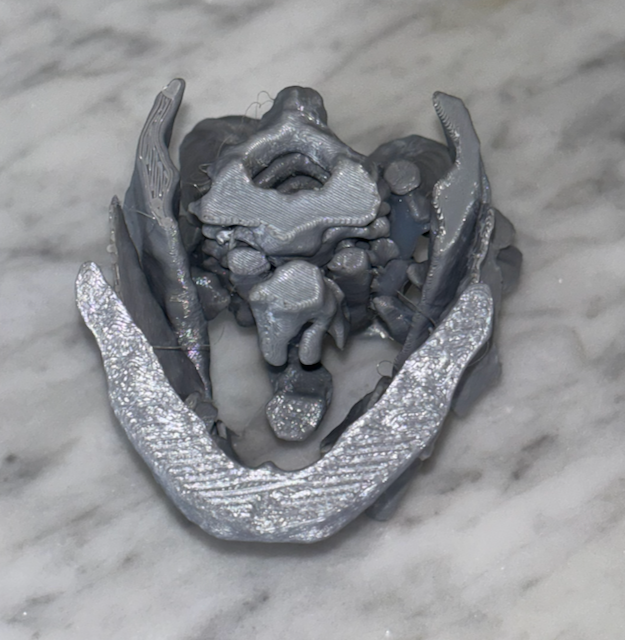
\includegraphics[width=0.46\textwidth]{imagenes/fantoma-v1-superior.png}
  \caption{Primera generación, impresa en piezas separadas y ensamblada con adhesivo. El ensamblado de múltiples piezas pequeñas resultó frágil y propenso a errores.}
  \label{fig:fantoma-v1}
  \begin{minipage}{\textwidth}
    \centering
    \normalsize Fuente: Elaboración propia.\\
  \end{minipage}
\end{figure}
 
La segunda generación abandonó el ensamblado de piezas y pasó a imprimir el modelo como un bloque, conservando la diferenciación por color de las estructuras. La Figura~\ref{fig:fantoma-v2} muestra un corte transversal en el que se distinguen la piel y el tejido graso subcutáneo, la musculatura cervical, la vértebra y, en tono claro, los músculos esternotiroideo y esternocleidomastoideo. Esta versión mejoró la integridad estructural respecto de la anterior, pero mantener el modelo cerrado impedía observar las estructuras internas.\\
 
\begin{figure}[H]
  \centering
  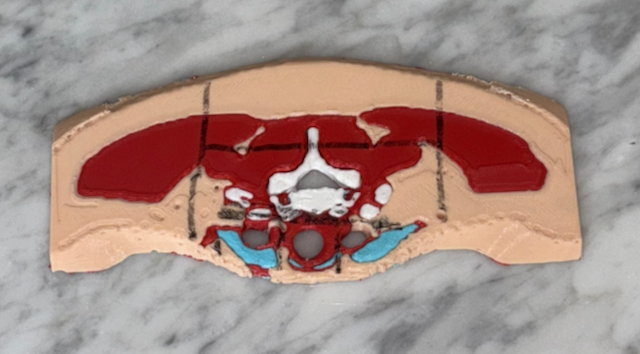
\includegraphics[width=0.72\textwidth]{imagenes/fantoma-v2-axial.png}
  \caption{Segunda generación, impresa como bloque con diferenciación por color. Se distinguen la piel y el tejido graso subcutáneo, la musculatura, la vértebra y los músculos esternotiroideo y esternocleidomastoideo.}
  \label{fig:fantoma-v2}
  \begin{minipage}{\textwidth}
    \centering
    \normalsize Fuente: Elaboración propia.\\
  \end{minipage}
\end{figure}
 
La tercera generación introdujo la división del modelo en láminas horizontales, lo que permitió inspeccionar el interior sin comprometer la integridad del conjunto. La orientación horizontal, sin embargo, trajo dos inconvenientes: exigía una gran cantidad de soportes de impresión, que encarecen el material y el tiempo y dejan marcas al retirarse, y repartía las estructuras del punto de incisión entre láminas, lo que dificultaba su lectura conjunta. Ambos problemas motivaron el paso a cortes verticales.\\
 
\begin{figure}[H]
  \centering
  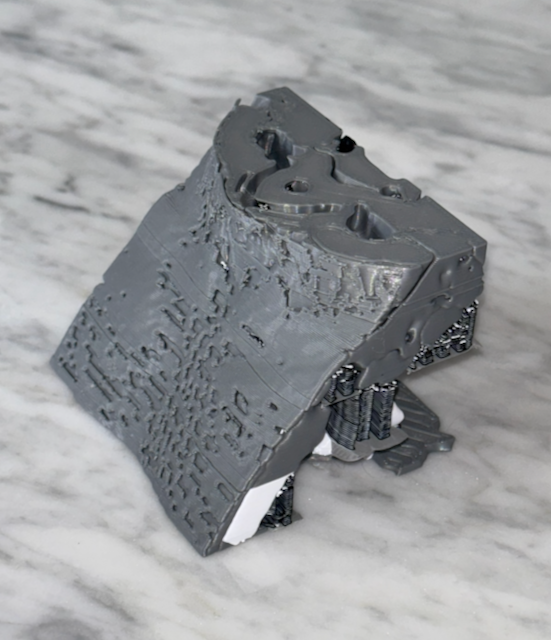
\includegraphics[width=0.6\textwidth]{imagenes/fantoma-v3.png}
  \caption{Tercera generación, dividida en láminas horizontales. La división permitió observar el interior, pero repartía las estructuras del punto de incisión entre distintas láminas.}
  \label{fig:fantoma-v3}
  \begin{minipage}{\textwidth}
    \centering
    \normalsize Fuente: Elaboración propia.\\
  \end{minipage}
\end{figure}
 
La cuarta generación, que constituye el resultado final, dividió el modelo en cuatro láminas verticales. Esta orientación resuelve los problemas anteriores: mantiene cada lámina dentro de las dimensiones de la cama de impresión, reduce los soportes necesarios y, al separarlas, expone en un mismo plano las estructuras internas del cuello, incluida la región del punto de incisión. La Figura~\ref{fig:fantoma-v4} muestra esta versión, en la que el mapa de colores del sistema diferencia cada tipo de tejido.\\
 
\begin{figure}[H]
  \centering
  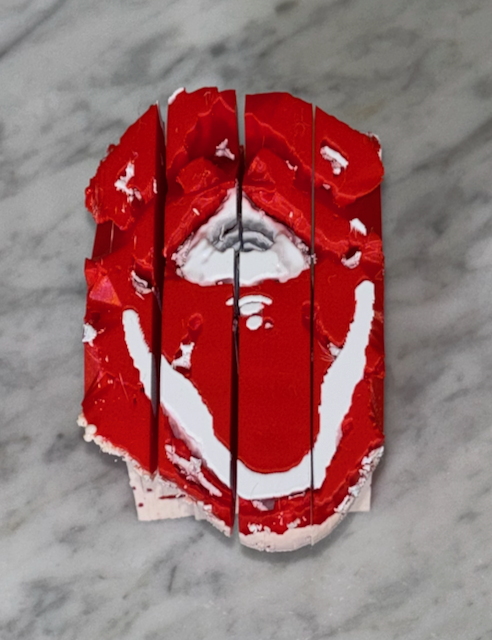
\includegraphics[width=0.46\textwidth]{imagenes/fantoma-v4-superior.png}\hfill
  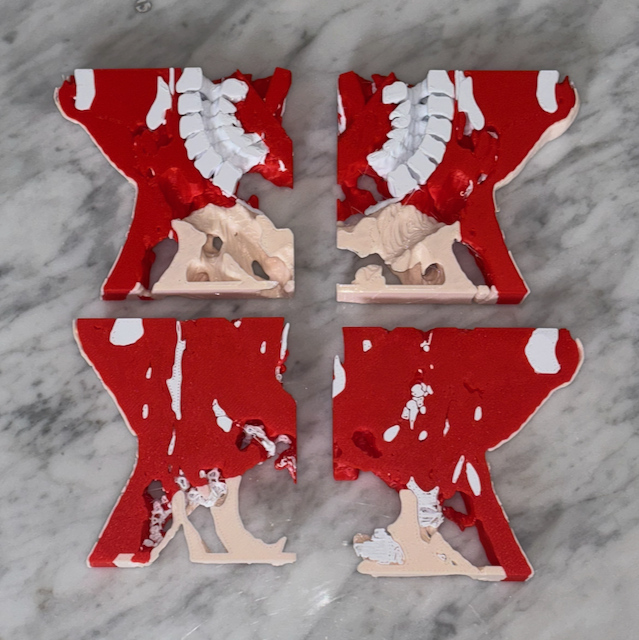
\includegraphics[width=0.46\textwidth]{imagenes/fantoma-v4-sagital.png}
  \caption{Cuarta generación del fantoma, el resultado final, dividida en cuatro láminas verticales. La orientación mantiene cada lámina dentro de la cama de impresión y deja a la vista las estructuras internas del cuello en un mismo plano.}
  \label{fig:fantoma-v4}
  \begin{minipage}{\textwidth}
    \centering
    \normalsize Fuente: Elaboración propia.\\
  \end{minipage}
\end{figure}
 
Los modelos se prepararon en el laminador PrusaSlicer y se imprimieron en una Prusa XL de múltiples cabezales, con boquilla de 0,4 mm, en PLA (ácido poliláctico, el filamento termoplástico más extendido en impresión doméstica) por deposición de material fundido, a un 60\% del tamaño anatómico real, escala necesaria para ajustar las piezas a las dimensiones de la cama de impresión. La pieza más detallada requirió aproximadamente 23,5 horas de impresión. El proceso no estuvo exento de dificultades: se produjeron fallos en los cabezales, cortes de suministro eléctrico y errores de \textit{firmware} de la impresora, que obligaron a repetir impresiones y prolongaron la fabricación. En todos los casos, las estructuras reproducen la anatomía individual del paciente de origen, que es precisamente la diversidad morfológica que los fantomas comerciales genéricos no ofrecen.\\

El material es el único insumo recurrente del proceso. A partir del filamento empleado, un rollo de PLA de 1,75 mm de diámetro a un valor de \$14.990 CLP por kilogramo, y considerando la escala de impresión al 60\%, un fantoma consume entre unos 274 y 297 gramos de filamento según el número de estructuras que se impriman, lo que equivale a entre \$4.100 y \$4.500 CLP aproximadamente. La cifra contrasta con el rango de USD 100 a más de USD 1.000 por modelo que la literatura reporta para los modelos anatómicos personalizados de referencia comercial (Capítulo~\ref{ch:problematica}), y confirma que el requisito de costo reducido se cumple con holgura.

Las impresiones se realizaron con un único material y con varios colores, lo que permite distinguir visualmente los tejidos pero mantiene una rigidez uniforme en toda la pieza. En consecuencia, los fantomas obtenidos habilitan la observación y el reconocimiento anatómico de la región de la cricotiroidotomía, pero no reproducen la consistencia diferenciada del tejido blando que requeriría practicar la incisión con realismo táctil. Esta limitación, anticipada en el Capítulo~\ref{ch:problematica}, se aborda entre las mejoras propuestas. La validación clínica del fantoma con la Dra. Marcela Garrido se encuentra pendiente.\\

\section{POSIBLES MEJORAS}

El sistema cumple los objetivos planteados para el producto, pero la evaluación realizada y la experiencia de uso del flujo permiten identificar varias líneas de mejora que exceden el alcance de este trabajo y quedan propuestas para su continuación.\\

\begin{enumerate}
  \item \textbf{Revisión asistida de vértebras y vía aérea:} el análisis de las correcciones del especialista mostró que la segmentación automática es aceptada sin retoques en el tejido blando, pero requiere revisión en las vértebras cervicales y en la tráquea. Incorporar al módulo una etapa de revisión guiada, que presente al usuario clínico precisamente esas ocho estructuras para su validación o ajuste antes de exportar, concentraría el esfuerzo humano donde el sistema efectivamente lo necesita y dejaría el resto del flujo automatizado.

  \item \textbf{Reducción del tiempo de manejo de archivos:} el desglose de tiempos mostró que la recuperación y escritura local de las estructuras consume la mayor parte del tiempo total, no por el volumen de datos ni por la red, sino por realizarse sobre más de cien archivos independientes. Optimizar la escritura local de estas máscaras es la mejora de mayor impacto por unidad de esfuerzo, y no requiere cambiar el motor de segmentación ni el hardware.

  \item \textbf{Evaluación con una referencia independiente:} la limitación metodológica identificada en este trabajo, esto es, que la segmentación de referencia deriva de la propia herramienta evaluada, solo puede resolverse con anotaciones elaboradas sin apoyo de segmentación automática, o bien con anotaciones de un segundo especialista sobre un subconjunto de casos. Ello permitiría cuantificar la precisión real del sistema y no solo su concordancia.

  \item \textbf{Fidelidad táctil de los materiales:} los materiales de impresión no reproducen la consistencia del tejido blando real, lo que limita el realismo de la incisión. Explorar la impresión con materiales flexibles o con combinaciones de distinta dureza, diferenciando por ejemplo piel, cartílago y vía aérea, permitiría aproximar mejor la sensación de la maniobra.

  \item \textbf{Automatización del corte:} el recorte del modelo se realiza hoy de forma manual mediante planos interactivos. Una selección automática de la región de interés, a partir de las estructuras del punto de incisión ya segmentadas, reduciría aún más la intervención del usuario.

  \item \textbf{Extensión a otras regiones anatómicas:} el flujo generaliza a otras zonas del cuerpo, pero la cobertura depende del conjunto de tareas de segmentación configurado. Ampliar y parametrizar ese conjunto permitiría aplicar el sistema a procedimientos distintos de la cricotiroidotomía sin modificar la arquitectura.
\end{enumerate}
\chapter{Conclusiones}
\label{ch:conclusiones}

\section{CUMPLIMIENTO DE LOS OBJETIVOS}

El problema que dio origen a este trabajo era concreto: la generación de fantomas anatómicos no estándar resultaba inviable a escala porque dependía de la segmentación manual de un especialista, un proceso que consume varias horas de trabajo experto por cada caso. Esa dependencia obligaba a los estudiantes de medicina a entrenar sobre los mismos modelos genéricos, sin exposición a la variabilidad anatómica que encontrarán en la práctica clínica.\\

El sistema desarrollado cierra esa brecha. A partir de una TC en formato NIfTI, produce de forma automatizada un conjunto de estructuras anatómicas segmentadas, recortadas y exportadas a archivos STL imprimibles, con un tiempo por caso cuya mediana se mantiene dentro del límite operacional fijado en los requisitos, aunque el promedio lo supera de forma marginal por la variabilidad de una de sus etapas. Lo que antes exigía la dedicación de un radiólogo durante horas se resuelve ahora sin intervención experta, mediante una interfaz guiada operable por personal médico sin formación en procesamiento de imágenes. El objetivo central del proyecto, por tanto, se cumple.\\

El recorrido completo quedó además validado físicamente. Los archivos generados por el sistema se imprimieron de manera efectiva, produciendo fantomas que reproducen la anatomía cervical individual de los casos de origen. Con ello, el flujo que va desde la imagen médica hasta el objeto tangible (adquisición, segmentación, exportación y fabricación) queda cubierto de extremo a extremo, que era precisamente el eslabón que la literatura revisada dejaba sin resolver de manera integrada \citep{bucking2017workflow}.\\

\section{PRINCIPALES HALLAZGOS}

El hallazgo de mayor peso de este trabajo fue inesperado. La evaluación comparativa se diseñó para determinar cuál de tres modelos segmenta con mayor precisión, pero al auditar los datos se constató que la segmentación de referencia no era una anotación manual independiente: el radiólogo la elaboró ejecutando TotalSegmentator y corrigiendo su salida. La evidencia es inequívoca, con estructuras que difieren entre la referencia y la salida automática en unas decenas de vóxeles sobre varios millones. Ello implica que las métricas de superposición no miden precisión frente a un patrón independiente, sino concordancia entre un modelo y una versión corregida de sí mismo, y que por tanto no pueden arbitrar de forma imparcial la comparación para la que fueron calculadas.\\

Constatar esto obligó a reconstruir el fundamento de la elección del motor sobre criterios ajenos a esas métricas. Ese fundamento resultó ser más sólido que el original y se detalla en el Capítulo~\ref{ch:resultados}: la autonomía para segmentar sin indicaciones manuales, la cobertura de las estructuras que delimitan el punto de incisión y el aval implícito del propio especialista, que eligió TotalSegmentator como punto de partida y aceptó su salida casi sin retoques. Ninguno de esos criterios descansa en la comparación contra la referencia.\\

Esa misma circunstancia abrió un análisis adicional. Al comparar la salida automática con la referencia corregida se puede identificar con exactitud dónde intervino el especialista: aceptó sin retoques la práctica totalidad del tejido blando, la musculatura, las glándulas, los ojos y los tejidos grasos, y concentró sus correcciones en las siete vértebras cervicales y en la tráquea, sin casos intermedios. El dato delimita dónde la segmentación automática es confiable y dónde requiere supervisión clínica, y lo hace sobre las estructuras que importan para la cricotiroidotomía. Es información accionable, recogida entre las mejoras propuestas.\\

Un hallazgo de orden metodológico surgió al examinar la cobertura de los modelos. Evaluados de forma nominal, MedSAM y YOLO parecían detectar la totalidad de las estructuras de referencia. Esa cifra resultó ser un artefacto: el coeficiente de Dice está indefinido cuando la máscara predicha y la de referencia están ambas vacías, y la convención le asigna el valor 1, de modo que un modelo obtiene una puntuación perfecta sobre las estructuras que el escáner no alcanza a cubrir, sin haber segmentado nada. Al excluirlas y exigir una superposición mínima real, la cobertura de YOLO cayó a un 13,4\%, reducida a envolturas externas y regiones de gran volumen. El análisis de sensibilidad al umbral mostró además que la cobertura de MedSAM se reduce a menos de la mitad al endurecer el criterio, mientras que la de TotalSegmentator se mantiene constante en los tres umbrales. De ahí una lección de alcance general: una cifra de cobertura no significa nada si no se declara el umbral que la sostiene y no se verifica que la referencia tenga contenido real.\\

Un último hallazgo emergió del desglose de tiempos del sistema integrado. La segmentación, que es la etapa computacionalmente exigente y la que justificó toda la infraestructura de cómputo remoto, resultó ser una fracción menor del tiempo total. La mayor parte se consume transfiriendo y administrando archivos, porque el sistema produce más de un centenar de máscaras independientes por caso. El cuello de botella no estaba donde el diseño inicial suponía, y ello reordenó las prioridades de optimización: el camino más rentable no pasa por más capacidad de cómputo sino por el manejo de los archivos.\\

Otra decisión de diseño quedó puesta a prueba durante la evaluación. TotalSegmentator dispone de una tarea adicional que habría cubierto las seis estructuras faltantes (mandíbula, arcadas dentarias, senos y cabeza) e igualado la referencia por completo. Se optó por no ejecutarla: ninguna de esas estructuras interviene en la cricotiroidotomía, y añadirlas habría mejorado una métrica a costa de más tiempo de procesamiento y una pieza más voluminosa de imprimir, sin aportar nada al fantoma. Lo que ordenó el diseño fue la utilidad del modelo para el procedimiento, por encima de la maximización de un indicador. El sistema demostró además no estar atado a la anatomía cervical: una TC de pie procesada a través del módulo completo, sin modificar el código, confirmó que la arquitectura generaliza y que la limitación reside en la configuración de las tareas, no en el diseño del flujo.\\

\section{LIMITACIONES DEL TRABAJO}

El alcance de lo logrado debe enunciarse con precisión, y la limitación principal es la ya expuesta. Al derivar la segmentación de referencia de la propia herramienta evaluada, este trabajo no puede afirmar cuál es la precisión del sistema frente a un patrón independiente. Puede afirmar que produce una segmentación que un especialista aceptó casi íntegramente, y que las alternativas consideradas no logran reproducirla ni operando en condiciones privilegiadas, pero no puede cuantificar cuánto se aparta de la anatomía real. Resolver esto exige anotaciones elaboradas sin apoyo de segmentación automática, o bien anotaciones independientes de un segundo especialista, y queda planteado como continuación necesaria.\\

Los fantomas impresos hasta la fecha son piezas rígidas de un único material, diferenciadas por color pero no por consistencia. Habilitan la observación y el reconocimiento anatómico de la región de interés, pero no reproducen la sensación táctil de la incisión sobre tejido blando, que es una de las competencias que el entrenamiento en cricotiroidotomía busca desarrollar. El fantoma es hoy una herramienta de estudio anatómico personalizado más que un simulador de la maniobra completa.\\

La validación clínica con el equipo médico se encuentra pendiente. Sin ella, la utilidad formativa del fantoma constituye una expectativa fundamentada en la literatura y en el criterio de diseño, pero no un resultado verificado con usuarios reales. Esta validación es, a juicio de los autores, la prioridad más urgente para la continuación del trabajo, por encima de cualquier mejora técnica adicional.\\

Por último, la base de evaluación se compone de diez casos, un número limitado para caracterizar el comportamiento del sistema frente a anatomías patológicas o atípicas, que son las que más se beneficiarían de un fantoma personalizado.\\

\section{PROYECCIÓN E IMPACTO}

Más allá del artefacto construido, el trabajo sugiere una forma distinta de entender el acceso al entrenamiento quirúrgico. Los fantomas comerciales son costosos, importados y anatómicamente uniformes; producir uno personalizado requería hasta ahora recursos que solo centros con financiamiento dedicado podían permitirse. El sistema desarrollado invierte esa lógica: se apoya íntegramente en software de código abierto y opera sobre imágenes médicas que las instituciones de salud ya poseen, generadas en el curso normal de la atención clínica. No exige adquirir modelos nuevos ni someter a ningún paciente a estudios adicionales, sino que reutiliza información existente.\\

Esto abre la posibilidad de que una institución constituya progresivamente una biblioteca de casos propios, en lugar de depender de un catálogo externo de modelos genéricos. Cada tomografía cervical archivada se convierte en un fantoma potencial, y el costo marginal de incorporar un caso nuevo pasa a ser el del material de impresión y el tiempo de uso de máquina. La diversidad anatómica sobre la que un estudiante puede entrenar deja de estar limitada por el presupuesto y pasa a estarlo únicamente por la disponibilidad de casos, que en un hospital es abundante.\\

Hay además una dimensión de autonomía. Un flujo construido sobre herramientas abiertas y ejecutable en equipamiento modesto puede ser adoptado, auditado y modificado por la propia institución, sin quedar atado a un proveedor ni a licencias que condicionen su continuidad. En un contexto donde los programas de simulación clínica en el país dependen mayoritariamente de material importado de alto costo, esa independencia tiene un peso real.\\

El camino por recorrer sigue siendo considerable, y las líneas de trabajo identificadas en el Capítulo~\ref{ch:resultados} lo delinean. El resultado central de esta memoria es que ese camino dejó de ser hipotético: el sistema funciona, el flujo es reproducible y el objeto físico existe.\\

% Ingenieros prefieren la bibliografia antes que los anexos

\cleardoublepage
\refstepcounter{chapter}
\addcontentsline{toc}{chapter}{\thechapter.\enspace\MakeUppercase{\bibname}}
{\noindent\bfseries\thechapter. \MakeUppercase{\bibname}\par}
\vspace{1em}
\bibliographystyle{agsm}
\bibliography{referencias}

\appendix % seguido de archivos de apendices
% Nota: \chapter{Anexos} en attachments/anexo_a.tex genera su propia entrada
% en el índice como "A. Anexos". No agregar otra entry manual aquí.
\cleardoublepage
\chapter{Anexos}
\label{ch:anexos}

\section{Repositorios del proyecto}
\label{ax:repositorios}

El código fuente del sistema está disponible en los siguientes repositorios:

\begin{enumerate}
  \item Módulos de 3D Slicer (segmentación y corte): \href{https://github.com/trodriguezam/modulo-fantoma}{\texttt{github.com/trodriguezam/modulo-fantoma}}
  \item Código de ejecución remota sobre GPU: \href{https://github.com/trodriguezam/MBX-remoto}{\texttt{github.com/trodriguezam/MBX-remoto}}
\end{enumerate}

Cada repositorio incluye un archivo \texttt{README} con las instrucciones de instalación y uso.    % archivo de apendice

%\input{apendice_b}    % otro archivo de apendice

% Declaración de uso de IA
\cleardoublepage
\addcontentsline{toc}{chapter}{\MakeUppercase{Declaración sobre el uso de inteligencia artificial}}
{\noindent\bfseries \MakeUppercase{Declaración sobre el uso de inteligencia artificial}\par}
\vspace{1em}

En la elaboración de este trabajo se utilizó la herramienta de inteligencia artificial generativa Claude, de Anthropic, como apoyo en dos frentes.\\

En la redacción del informe se empleó para revisar ortografía y gramática, sugerir formulaciones y ordenar la estructura de algunas secciones. El contenido técnico, los resultados y las conclusiones son responsabilidad de los autores, que revisaron y validaron cada texto incorporado.\\

En el desarrollo de los módulos se empleó para asistir en la escritura y la depuración del código. Los autores verificaron el funcionamiento del sistema resultante.\\

Este uso, propio de la producción del trabajo, es distinto de los modelos de inteligencia artificial que son objeto de estudio del proyecto (TotalSegmentator, MedSAM y YOLO), evaluados y documentados en los capítulos correspondientes.

\end{document}

%%%%%%%%%%%%%%%%%%%%%%%%%%%%%%%%%%%%%%%%%%%%%%%%%%%%%%%%%%%%
